\documentclass[twoside]{book}

% Packages required by doxygen
\usepackage{fixltx2e}
\usepackage{calc}
\usepackage{doxygen}
\usepackage[export]{adjustbox} % also loads graphicx
\usepackage{graphicx}
\usepackage[utf8]{inputenc}
\usepackage{makeidx}
\usepackage{multicol}
\usepackage{multirow}
\PassOptionsToPackage{warn}{textcomp}
\usepackage{textcomp}
\usepackage[nointegrals]{wasysym}
\usepackage[table]{xcolor}

% Font selection
\usepackage[T1]{fontenc}
\usepackage[scaled=.90]{helvet}
\usepackage{courier}
\usepackage{amssymb}
\usepackage{sectsty}
\renewcommand{\familydefault}{\sfdefault}
\allsectionsfont{%
  \fontseries{bc}\selectfont%
  \color{darkgray}%
}
\renewcommand{\DoxyLabelFont}{%
  \fontseries{bc}\selectfont%
  \color{darkgray}%
}
\newcommand{\+}{\discretionary{\mbox{\scriptsize$\hookleftarrow$}}{}{}}

% Page & text layout
\usepackage{geometry}
\geometry{%
  a4paper,%
  top=2.5cm,%
  bottom=2.5cm,%
  left=2.5cm,%
  right=2.5cm%
}
\tolerance=750
\hfuzz=15pt
\hbadness=750
\setlength{\emergencystretch}{15pt}
\setlength{\parindent}{0cm}
\setlength{\parskip}{3ex plus 2ex minus 2ex}
\makeatletter
\renewcommand{\paragraph}{%
  \@startsection{paragraph}{4}{0ex}{-1.0ex}{1.0ex}{%
    \normalfont\normalsize\bfseries\SS@parafont%
  }%
}
\renewcommand{\subparagraph}{%
  \@startsection{subparagraph}{5}{0ex}{-1.0ex}{1.0ex}{%
    \normalfont\normalsize\bfseries\SS@subparafont%
  }%
}
\makeatother

% Headers & footers
\usepackage{fancyhdr}
\pagestyle{fancyplain}
\fancyhead[LE]{\fancyplain{}{\bfseries\thepage}}
\fancyhead[CE]{\fancyplain{}{}}
\fancyhead[RE]{\fancyplain{}{\bfseries\leftmark}}
\fancyhead[LO]{\fancyplain{}{\bfseries\rightmark}}
\fancyhead[CO]{\fancyplain{}{}}
\fancyhead[RO]{\fancyplain{}{\bfseries\thepage}}
\fancyfoot[LE]{\fancyplain{}{}}
\fancyfoot[CE]{\fancyplain{}{}}
\fancyfoot[RE]{\fancyplain{}{\bfseries\scriptsize Generated by Doxygen }}
\fancyfoot[LO]{\fancyplain{}{\bfseries\scriptsize Generated by Doxygen }}
\fancyfoot[CO]{\fancyplain{}{}}
\fancyfoot[RO]{\fancyplain{}{}}
\renewcommand{\footrulewidth}{0.4pt}
\renewcommand{\chaptermark}[1]{%
  \markboth{#1}{}%
}
\renewcommand{\sectionmark}[1]{%
  \markright{\thesection\ #1}%
}

% Indices & bibliography
\usepackage{natbib}
\usepackage[titles]{tocloft}
\setcounter{tocdepth}{3}
\setcounter{secnumdepth}{5}
\makeindex

% Hyperlinks (required, but should be loaded last)
\usepackage{ifpdf}
\ifpdf
  \usepackage[pdftex,pagebackref=true]{hyperref}
\else
  \usepackage[ps2pdf,pagebackref=true]{hyperref}
\fi
\hypersetup{%
  colorlinks=true,%
  linkcolor=blue,%
  citecolor=blue,%
  unicode%
}

% Custom commands
\newcommand{\clearemptydoublepage}{%
  \newpage{\pagestyle{empty}\cleardoublepage}%
}

\usepackage{caption}
\captionsetup{labelsep=space,justification=centering,font={bf},singlelinecheck=off,skip=4pt,position=top}

%===== C O N T E N T S =====

\begin{document}

% Titlepage & ToC
\hypersetup{pageanchor=false,
             bookmarksnumbered=true,
             pdfencoding=unicode
            }
\pagenumbering{alph}
\begin{titlepage}
\vspace*{7cm}
\begin{center}%
{\Large A\+P\+P\+B\+IT \\[1ex]\large 1.\+0.\+0 }\\
\vspace*{1cm}
{\large Generated by Doxygen 1.8.14}\\
\end{center}
\end{titlepage}
\clearemptydoublepage
\pagenumbering{roman}
\tableofcontents
\clearemptydoublepage
\pagenumbering{arabic}
\hypersetup{pageanchor=true}

%--- Begin generated contents ---
\chapter{Hierarchical Index}
\section{Class Hierarchy}
This inheritance list is sorted roughly, but not completely, alphabetically\+:\begin{DoxyCompactList}
\item C\+I\+\_\+\+Controller\begin{DoxyCompactList}
\item \contentsline{section}{Admin}{\pageref{class_admin}}{}
\item \contentsline{section}{Deelnemer}{\pageref{class_deelnemer}}{}
\item \contentsline{section}{Jaargang}{\pageref{class_jaargang}}{}
\item \contentsline{section}{Keuzemogelijkheid}{\pageref{class_keuzemogelijkheid}}{}
\item \contentsline{section}{Keuzeoptie}{\pageref{class_keuzeoptie}}{}
\item \contentsline{section}{Keuze\+Optie\+Van\+Deelnemer}{\pageref{class_keuze_optie_van_deelnemer}}{}
\item \contentsline{section}{Mail}{\pageref{class_mail}}{}
\item \contentsline{section}{Main}{\pageref{class_main}}{}
\item \contentsline{section}{Plaats}{\pageref{class_plaats}}{}
\item \contentsline{section}{Shiften}{\pageref{class_shiften}}{}
\item \contentsline{section}{Taken}{\pageref{class_taken}}{}
\item \contentsline{section}{Vrijwilliger}{\pageref{class_vrijwilliger}}{}
\end{DoxyCompactList}
\item C\+I\+\_\+\+Model\begin{DoxyCompactList}
\item \contentsline{section}{Beheer\+\_\+model}{\pageref{class_beheer__model}}{}
\item \contentsline{section}{csv\+\_\+model}{\pageref{classcsv__model}}{}
\item \contentsline{section}{Jaargang\+\_\+model}{\pageref{class_jaargang__model}}{}
\item \contentsline{section}{Keuzemogelijkheid\+\_\+\+Model}{\pageref{class_keuzemogelijkheid___model}}{}
\item \contentsline{section}{Keuzeoptie\+\_\+\+Model}{\pageref{class_keuzeoptie___model}}{}
\item \contentsline{section}{Keuzeoptie\+Van\+Deelnemer\+\_\+\+Model}{\pageref{class_keuzeoptie_van_deelnemer___model}}{}
\item \contentsline{section}{Mailherinnering\+\_\+model}{\pageref{class_mailherinnering__model}}{}
\item \contentsline{section}{Mailsjabloon\+\_\+model}{\pageref{class_mailsjabloon__model}}{}
\item \contentsline{section}{Persoon\+\_\+model}{\pageref{class_persoon__model}}{}
\item \contentsline{section}{Persoon\+In\+Herinnering\+\_\+model}{\pageref{class_persoon_in_herinnering__model}}{}
\item \contentsline{section}{Plaats\+\_\+model}{\pageref{class_plaats__model}}{}
\item \contentsline{section}{Shiften\+\_\+\+Model}{\pageref{class_shiften___model}}{}
\item \contentsline{section}{Taken\+\_\+\+Model}{\pageref{class_taken___model}}{}
\item \contentsline{section}{Vrijwilligers\+In\+Shift\+\_\+\+Model}{\pageref{class_vrijwilligers_in_shift___model}}{}
\end{DoxyCompactList}
\end{DoxyCompactList}

\chapter{Data Structure Index}
\section{Class List}
Here are the classes, structs, unions and interfaces with brief descriptions\+:\begin{DoxyCompactList}
\item\contentsline{section}{\mbox{\hyperlink{class_admin}{Admin}} \\*Controller voor administratorfunctionaliteiten }{\pageref{class_admin}}{}
\item\contentsline{section}{\mbox{\hyperlink{class_beheer__model}{Beheer\+\_\+model}} }{\pageref{class_beheer__model}}{}
\item\contentsline{section}{\mbox{\hyperlink{classcsv__model}{csv\+\_\+model}} }{\pageref{classcsv__model}}{}
\item\contentsline{section}{\mbox{\hyperlink{class_deelnemer}{Deelnemer}} \\*Constructor voor deelnemer functionaliteiten }{\pageref{class_deelnemer}}{}
\item\contentsline{section}{\mbox{\hyperlink{class_jaargang}{Jaargang}} \\*Controller voor jaargangfunctionaliteiten }{\pageref{class_jaargang}}{}
\item\contentsline{section}{\mbox{\hyperlink{class_jaargang__model}{Jaargang\+\_\+model}} }{\pageref{class_jaargang__model}}{}
\item\contentsline{section}{\mbox{\hyperlink{class_keuzemogelijkheid}{Keuzemogelijkheid}} \\*Controller voor keuzemogelijkheidfunctionaliteiten }{\pageref{class_keuzemogelijkheid}}{}
\item\contentsline{section}{\mbox{\hyperlink{class_keuzemogelijkheid___model}{Keuzemogelijkheid\+\_\+\+Model}} \\*Klasse voor gegevens van de activiteiten te beheren }{\pageref{class_keuzemogelijkheid___model}}{}
\item\contentsline{section}{\mbox{\hyperlink{class_keuzeoptie}{Keuzeoptie}} }{\pageref{class_keuzeoptie}}{}
\item\contentsline{section}{\mbox{\hyperlink{class_keuzeoptie___model}{Keuzeoptie\+\_\+\+Model}} \\*Model voor de database manipultie van de tabel \mbox{\hyperlink{class_keuzeoptie}{Keuzeoptie}} }{\pageref{class_keuzeoptie___model}}{}
\item\contentsline{section}{\mbox{\hyperlink{class_keuze_optie_van_deelnemer}{Keuze\+Optie\+Van\+Deelnemer}} \\*Controller voor functionaliteiten van keuzeoptie voor deelnemer }{\pageref{class_keuze_optie_van_deelnemer}}{}
\item\contentsline{section}{\mbox{\hyperlink{class_keuzeoptie_van_deelnemer___model}{Keuzeoptie\+Van\+Deelnemer\+\_\+\+Model}} }{\pageref{class_keuzeoptie_van_deelnemer___model}}{}
\item\contentsline{section}{\mbox{\hyperlink{class_mail}{Mail}} \\*Controller voor mailfunctionaliteiten }{\pageref{class_mail}}{}
\item\contentsline{section}{\mbox{\hyperlink{class_mailherinnering__model}{Mailherinnering\+\_\+model}} }{\pageref{class_mailherinnering__model}}{}
\item\contentsline{section}{\mbox{\hyperlink{class_mailsjabloon__model}{Mailsjabloon\+\_\+model}} }{\pageref{class_mailsjabloon__model}}{}
\item\contentsline{section}{\mbox{\hyperlink{class_main}{Main}} \\*Controller voor loginfunctionaliteit }{\pageref{class_main}}{}
\item\contentsline{section}{\mbox{\hyperlink{class_persoon__model}{Persoon\+\_\+model}} }{\pageref{class_persoon__model}}{}
\item\contentsline{section}{\mbox{\hyperlink{class_persoon_in_herinnering__model}{Persoon\+In\+Herinnering\+\_\+model}} }{\pageref{class_persoon_in_herinnering__model}}{}
\item\contentsline{section}{\mbox{\hyperlink{class_plaats}{Plaats}} \\*Controller voor plaats }{\pageref{class_plaats}}{}
\item\contentsline{section}{\mbox{\hyperlink{class_plaats__model}{Plaats\+\_\+model}} }{\pageref{class_plaats__model}}{}
\item\contentsline{section}{\mbox{\hyperlink{class_shiften}{Shiften}} \\*Controller voor shiften }{\pageref{class_shiften}}{}
\item\contentsline{section}{\mbox{\hyperlink{class_shiften___model}{Shiften\+\_\+\+Model}} \\*Model voor het beheren van de tabel shiften in de database }{\pageref{class_shiften___model}}{}
\item\contentsline{section}{\mbox{\hyperlink{class_taken}{Taken}} \\*Controller voor taken }{\pageref{class_taken}}{}
\item\contentsline{section}{\mbox{\hyperlink{class_taken___model}{Taken\+\_\+\+Model}} \\*Model voor beheren van de tabel taken van de database }{\pageref{class_taken___model}}{}
\item\contentsline{section}{\mbox{\hyperlink{class_vrijwilliger}{Vrijwilliger}} \\*Controller voor vrijwilligersfunctionaliteiten }{\pageref{class_vrijwilliger}}{}
\item\contentsline{section}{\mbox{\hyperlink{class_vrijwilligers_in_shift___model}{Vrijwilligers\+In\+Shift\+\_\+\+Model}} \\*Model voor beheren van de tabel shift van de database }{\pageref{class_vrijwilligers_in_shift___model}}{}
\end{DoxyCompactList}

\chapter{File Index}
\section{File List}
Here is a list of all files with brief descriptions\+:\begin{DoxyCompactList}
\item\contentsline{section}{application/controllers/\mbox{\hyperlink{_admin_8php}{Admin.\+php}} }{\pageref{_admin_8php}}{}
\item\contentsline{section}{application/controllers/\mbox{\hyperlink{_deelnemer_8php}{Deelnemer.\+php}} }{\pageref{_deelnemer_8php}}{}
\item\contentsline{section}{application/controllers/\mbox{\hyperlink{_jaargang_8php}{Jaargang.\+php}} }{\pageref{_jaargang_8php}}{}
\item\contentsline{section}{application/controllers/\mbox{\hyperlink{_keuzemogelijkheid_8php}{Keuzemogelijkheid.\+php}} }{\pageref{_keuzemogelijkheid_8php}}{}
\item\contentsline{section}{application/controllers/\mbox{\hyperlink{_keuzeoptie_8php}{Keuzeoptie.\+php}} }{\pageref{_keuzeoptie_8php}}{}
\item\contentsline{section}{application/controllers/\mbox{\hyperlink{_keuzeoptie_van_deelnemer_8php}{Keuzeoptie\+Van\+Deelnemer.\+php}} }{\pageref{_keuzeoptie_van_deelnemer_8php}}{}
\item\contentsline{section}{application/controllers/\mbox{\hyperlink{_mail_8php}{Mail.\+php}} }{\pageref{_mail_8php}}{}
\item\contentsline{section}{application/controllers/\mbox{\hyperlink{_main_8php}{Main.\+php}} }{\pageref{_main_8php}}{}
\item\contentsline{section}{application/controllers/\mbox{\hyperlink{_plaats_8php}{Plaats.\+php}} }{\pageref{_plaats_8php}}{}
\item\contentsline{section}{application/controllers/\mbox{\hyperlink{_shiften_8php}{Shiften.\+php}} }{\pageref{_shiften_8php}}{}
\item\contentsline{section}{application/controllers/\mbox{\hyperlink{_taken_8php}{Taken.\+php}} }{\pageref{_taken_8php}}{}
\item\contentsline{section}{application/controllers/\mbox{\hyperlink{_vrijwilliger_8php}{Vrijwilliger.\+php}} }{\pageref{_vrijwilliger_8php}}{}
\item\contentsline{section}{application/helpers/\mbox{\hyperlink{_m_y__form__helper_8php}{M\+Y\+\_\+form\+\_\+helper.\+php}} }{\pageref{_m_y__form__helper_8php}}{}
\item\contentsline{section}{application/models/\mbox{\hyperlink{_beheer__model_8php}{Beheer\+\_\+model.\+php}} }{\pageref{_beheer__model_8php}}{}
\item\contentsline{section}{application/models/\mbox{\hyperlink{_c_s_v__model_8php}{C\+S\+V\+\_\+model.\+php}} }{\pageref{_c_s_v__model_8php}}{}
\item\contentsline{section}{application/models/\mbox{\hyperlink{_jaargang__model_8php}{Jaargang\+\_\+model.\+php}} }{\pageref{_jaargang__model_8php}}{}
\item\contentsline{section}{application/models/\mbox{\hyperlink{_keuzemogelijkheid__model_8php}{Keuzemogelijkheid\+\_\+model.\+php}} }{\pageref{_keuzemogelijkheid__model_8php}}{}
\item\contentsline{section}{application/models/\mbox{\hyperlink{_keuzeoptie__model_8php}{Keuzeoptie\+\_\+model.\+php}} }{\pageref{_keuzeoptie__model_8php}}{}
\item\contentsline{section}{application/models/\mbox{\hyperlink{_keuzeoptie_van_deelnemer__model_8php}{Keuzeoptie\+Van\+Deelnemer\+\_\+model.\+php}} }{\pageref{_keuzeoptie_van_deelnemer__model_8php}}{}
\item\contentsline{section}{application/models/\mbox{\hyperlink{_mailherinnering__model_8php}{Mailherinnering\+\_\+model.\+php}} }{\pageref{_mailherinnering__model_8php}}{}
\item\contentsline{section}{application/models/\mbox{\hyperlink{_mailsjabloon__model_8php}{Mailsjabloon\+\_\+model.\+php}} }{\pageref{_mailsjabloon__model_8php}}{}
\item\contentsline{section}{application/models/\mbox{\hyperlink{_persoon__model_8php}{Persoon\+\_\+model.\+php}} }{\pageref{_persoon__model_8php}}{}
\item\contentsline{section}{application/models/\mbox{\hyperlink{_persoon_in_herinnering__model_8php}{Persoon\+In\+Herinnering\+\_\+model.\+php}} }{\pageref{_persoon_in_herinnering__model_8php}}{}
\item\contentsline{section}{application/models/\mbox{\hyperlink{_plaats__model_8php}{Plaats\+\_\+model.\+php}} }{\pageref{_plaats__model_8php}}{}
\item\contentsline{section}{application/models/\mbox{\hyperlink{_shiften__model_8php}{Shiften\+\_\+model.\+php}} }{\pageref{_shiften__model_8php}}{}
\item\contentsline{section}{application/models/\mbox{\hyperlink{_soort__model_8php}{Soort\+\_\+model.\+php}} }{\pageref{_soort__model_8php}}{}
\item\contentsline{section}{application/models/\mbox{\hyperlink{_taken__model_8php}{Taken\+\_\+model.\+php}} }{\pageref{_taken__model_8php}}{}
\item\contentsline{section}{application/models/\mbox{\hyperlink{_vervoerswijze__model_8php}{Vervoerswijze\+\_\+model.\+php}} }{\pageref{_vervoerswijze__model_8php}}{}
\item\contentsline{section}{application/models/\mbox{\hyperlink{_vrijwilligers_in_shift__model_8php}{Vrijwilligers\+In\+Shift\+\_\+model.\+php}} }{\pageref{_vrijwilligers_in_shift__model_8php}}{}
\end{DoxyCompactList}

\chapter{Data Structure Documentation}
\hypertarget{class_admin}{}\section{Admin Class Reference}
\label{class_admin}\index{Admin@{Admin}}


Controller voor administratorfunctionaliteiten.  


Inheritance diagram for Admin\+:\begin{figure}[H]
\begin{center}
\leavevmode
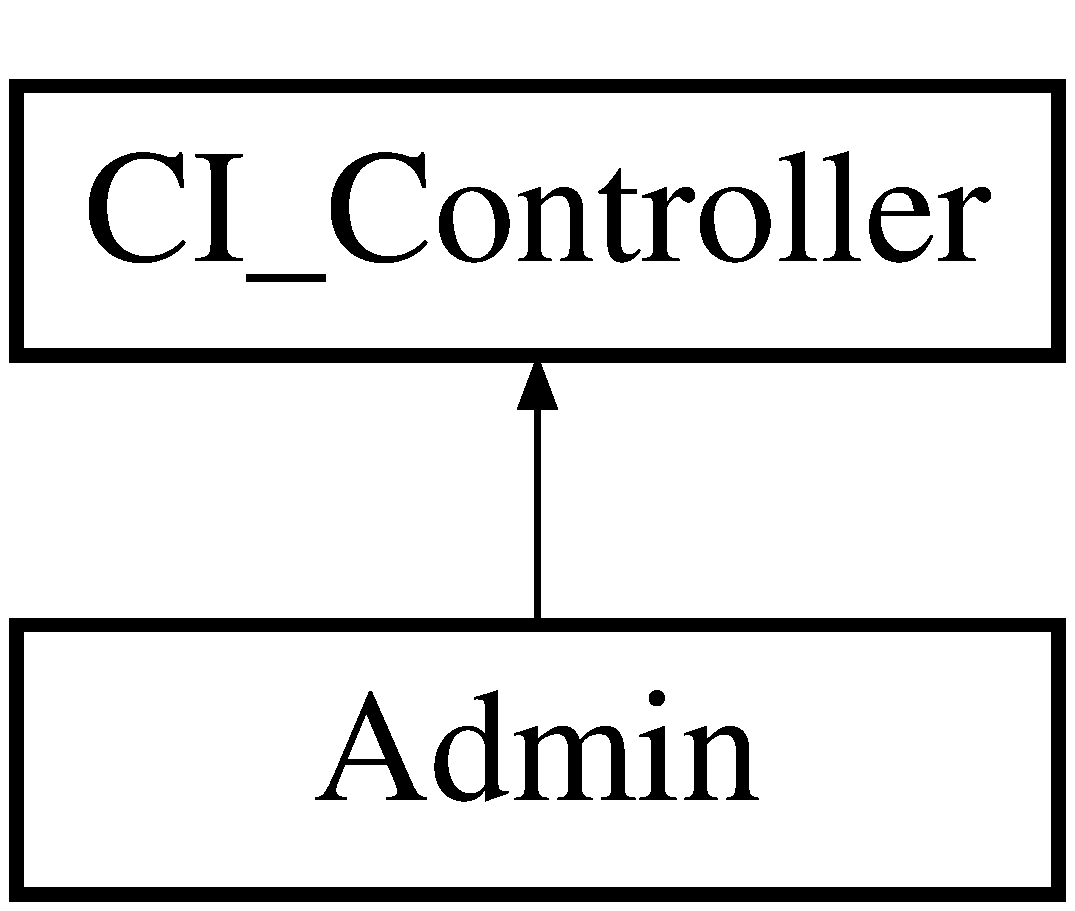
\includegraphics[height=2.000000cm]{class_admin}
\end{center}
\end{figure}
\subsection*{Public Member Functions}
\begin{DoxyCompactItemize}
\item 
\mbox{\hyperlink{class_admin_a14eb545baec47d1bccb823fdcea061d4}{\+\_\+\+\_\+construct}} ()
\item 
\mbox{\hyperlink{class_admin_ae7187e96036e6bd23086e02b936b214a}{index}} ()
\item 
\mbox{\hyperlink{class_admin_a7c5b27650e2fd63227f09ece49beb2e9}{dash}} (\$view=null, \$extras=null)
\item 
\mbox{\hyperlink{class_admin_ae84deedea35076345e2e892ea0d60413}{login}} (\$username=null, \$pass=null)
\item 
\mbox{\hyperlink{class_admin_a3a644a6067cccdf84a5649a7777c1197}{checkpass}} (\$id=null, \$pass=null)
\item 
\mbox{\hyperlink{class_admin_ac008e1e771793cdd2b8223eec46061ae}{logout}} ()
\item 
\mbox{\hyperlink{class_admin_a5c7b585615c86fd80fe4b2dd8e282da0}{update}} ()
\item 
\mbox{\hyperlink{class_admin_af559704017572a72fef6280a651e1245}{delete}} (\$id)
\item 
\mbox{\Hypertarget{class_admin_a6f3af7077b5bdaee0e8d4b43c0af9094}\label{class_admin_a6f3af7077b5bdaee0e8d4b43c0af9094}} 
\mbox{\hyperlink{class_admin_a6f3af7077b5bdaee0e8d4b43c0af9094}{excel}} ()
\begin{DoxyCompactList}\small\item\em lees een C\+SV bestand in met deelnemers/vrijwilligers en voeg deze toe aan de database \end{DoxyCompactList}\item 
\mbox{\Hypertarget{class_admin_a1842b1e31f070f58cc1a494739708244}\label{class_admin_a1842b1e31f070f58cc1a494739708244}} 
{\bfseries get\+\_\+\+Niet\+Ingeschreven} ()
\end{DoxyCompactItemize}


\subsection{Detailed Description}
Controller voor administratorfunctionaliteiten. 

\subsection{Constructor \& Destructor Documentation}
\mbox{\Hypertarget{class_admin_a14eb545baec47d1bccb823fdcea061d4}\label{class_admin_a14eb545baec47d1bccb823fdcea061d4}} 
\index{Admin@{Admin}!\+\_\+\+\_\+construct@{\+\_\+\+\_\+construct}}
\index{\+\_\+\+\_\+construct@{\+\_\+\+\_\+construct}!Admin@{Admin}}
\subsubsection{\texorpdfstring{\+\_\+\+\_\+construct()}{\_\_construct()}}
{\footnotesize\ttfamily Admin\+::\+\_\+\+\_\+construct (\begin{DoxyParamCaption}{ }\end{DoxyParamCaption})}

Default Constructor 

\subsection{Member Function Documentation}
\mbox{\Hypertarget{class_admin_a3a644a6067cccdf84a5649a7777c1197}\label{class_admin_a3a644a6067cccdf84a5649a7777c1197}} 
\index{Admin@{Admin}!checkpass@{checkpass}}
\index{checkpass@{checkpass}!Admin@{Admin}}
\subsubsection{\texorpdfstring{checkpass()}{checkpass()}}
{\footnotesize\ttfamily Admin\+::checkpass (\begin{DoxyParamCaption}\item[{}]{\$id = {\ttfamily null},  }\item[{}]{\$pass = {\ttfamily null} }\end{DoxyParamCaption})}

Login A\+PI call, print return waarde op scherm 
\begin{DoxyParams}[1]{Parameters}
id & {\em \$id} & Id van gebruiker \\
\hline
string & {\em \$pass} & Wachtwoord van gebruiker \\
\hline
\end{DoxyParams}
\mbox{\Hypertarget{class_admin_a7c5b27650e2fd63227f09ece49beb2e9}\label{class_admin_a7c5b27650e2fd63227f09ece49beb2e9}} 
\index{Admin@{Admin}!dash@{dash}}
\index{dash@{dash}!Admin@{Admin}}
\subsubsection{\texorpdfstring{dash()}{dash()}}
{\footnotesize\ttfamily Admin\+::dash (\begin{DoxyParamCaption}\item[{}]{\$view = {\ttfamily null},  }\item[{}]{\$extras = {\ttfamily null} }\end{DoxyParamCaption})}

Container voor alle dashbord schermen van administrator 
\begin{DoxyParams}[1]{Parameters}
string & {\em \$view} & Scherm dat opgeroepen word in het dashbord van administrator \\
\hline
string & {\em \$extras} & Optionele parameters \\
\hline
\end{DoxyParams}
Doorverwijzen naar de pagina waarop keuzemogelijkheden worden aangepast.

plaatsen inladen voor dropdown list

Doorverwijzen naar de pagina waarop keuzemogelijkheden worden aangemaakt.

jaren inladen voor dropdown list

plaatsen inladen voor dropdown list

Doorverwijzen naar de pagina waarop keuzeopties worden aangemaakt en aangepast.

plaatsen inladen voor dropdown list

kiezen of we een keuzeoptie moeten aanmaken of aanpassen en daarna alle gegevens ophalen.

Aanmaken van een keuzeoptie

Aanpassen van een keuzeoptie

Weergeven van alle keuzemogelijkheden voor een bepaald jaargang.

Als er geen jaargang meegegeven wordt, word je doorverwezen naar de home-\/pagina

Weergeven van alle taken voor een bepaalde keuzemogelijkheid.

Als er geen keuzemogelijkheid meegegeven wordt, word je doorverwezen naar de home-\/pagina

Doorverwijzen naar de pagina waarop taken worden aangemaakt en aangepast.

Doorverwijzen naar de pagina waarop shiften worden aangemaakt en aangepast.

De index pagina zal geladen worden als er te weinig info wordt meegegeven. \mbox{\Hypertarget{class_admin_af559704017572a72fef6280a651e1245}\label{class_admin_af559704017572a72fef6280a651e1245}} 
\index{Admin@{Admin}!delete@{delete}}
\index{delete@{delete}!Admin@{Admin}}
\subsubsection{\texorpdfstring{delete()}{delete()}}
{\footnotesize\ttfamily Admin\+::delete (\begin{DoxyParamCaption}\item[{}]{\$id }\end{DoxyParamCaption})}

Verwijderd de administrator 
\begin{DoxyParams}[1]{Parameters}
int & {\em \$id} & Id van gebruiker \\
\hline
\end{DoxyParams}
\mbox{\Hypertarget{class_admin_ae7187e96036e6bd23086e02b936b214a}\label{class_admin_ae7187e96036e6bd23086e02b936b214a}} 
\index{Admin@{Admin}!index@{index}}
\index{index@{index}!Admin@{Admin}}
\subsubsection{\texorpdfstring{index()}{index()}}
{\footnotesize\ttfamily Admin\+::index (\begin{DoxyParamCaption}{ }\end{DoxyParamCaption})}

Laad loginscherm voor administrator \mbox{\Hypertarget{class_admin_ae84deedea35076345e2e892ea0d60413}\label{class_admin_ae84deedea35076345e2e892ea0d60413}} 
\index{Admin@{Admin}!login@{login}}
\index{login@{login}!Admin@{Admin}}
\subsubsection{\texorpdfstring{login()}{login()}}
{\footnotesize\ttfamily Admin\+::login (\begin{DoxyParamCaption}\item[{}]{\$username = {\ttfamily null},  }\item[{}]{\$pass = {\ttfamily null} }\end{DoxyParamCaption})}

Login A\+PI call, print return waarde op scherm 
\begin{DoxyParams}[1]{Parameters}
string & {\em \$username} & Gebruikersnaam van gebruiker \\
\hline
string & {\em \$pass} & Wachtwoord van gebruiker \\
\hline
\end{DoxyParams}
\mbox{\Hypertarget{class_admin_ac008e1e771793cdd2b8223eec46061ae}\label{class_admin_ac008e1e771793cdd2b8223eec46061ae}} 
\index{Admin@{Admin}!logout@{logout}}
\index{logout@{logout}!Admin@{Admin}}
\subsubsection{\texorpdfstring{logout()}{logout()}}
{\footnotesize\ttfamily Admin\+::logout (\begin{DoxyParamCaption}{ }\end{DoxyParamCaption})}

Meld administrator af \mbox{\Hypertarget{class_admin_a5c7b585615c86fd80fe4b2dd8e282da0}\label{class_admin_a5c7b585615c86fd80fe4b2dd8e282da0}} 
\index{Admin@{Admin}!update@{update}}
\index{update@{update}!Admin@{Admin}}
\subsubsection{\texorpdfstring{update()}{update()}}
{\footnotesize\ttfamily Admin\+::update (\begin{DoxyParamCaption}{ }\end{DoxyParamCaption})}

Update administratorgegevens 

The documentation for this class was generated from the following file\+:\begin{DoxyCompactItemize}
\item 
E\+:/\+D\+R\+I\+V\+E/\+C\+O\+L\+L\+E\+G\+E/\+T\+M/\+P0202/\+K\+P0201/\+R\+E\+P\+O/application/controllers/Admin.\+php\end{DoxyCompactItemize}

\hypertarget{class_beheer__model}{}\section{Beheer\+\_\+model Class Reference}
\label{class_beheer__model}\index{Beheer\+\_\+model@{Beheer\+\_\+model}}
Inheritance diagram for Beheer\+\_\+model\+:\begin{figure}[H]
\begin{center}
\leavevmode
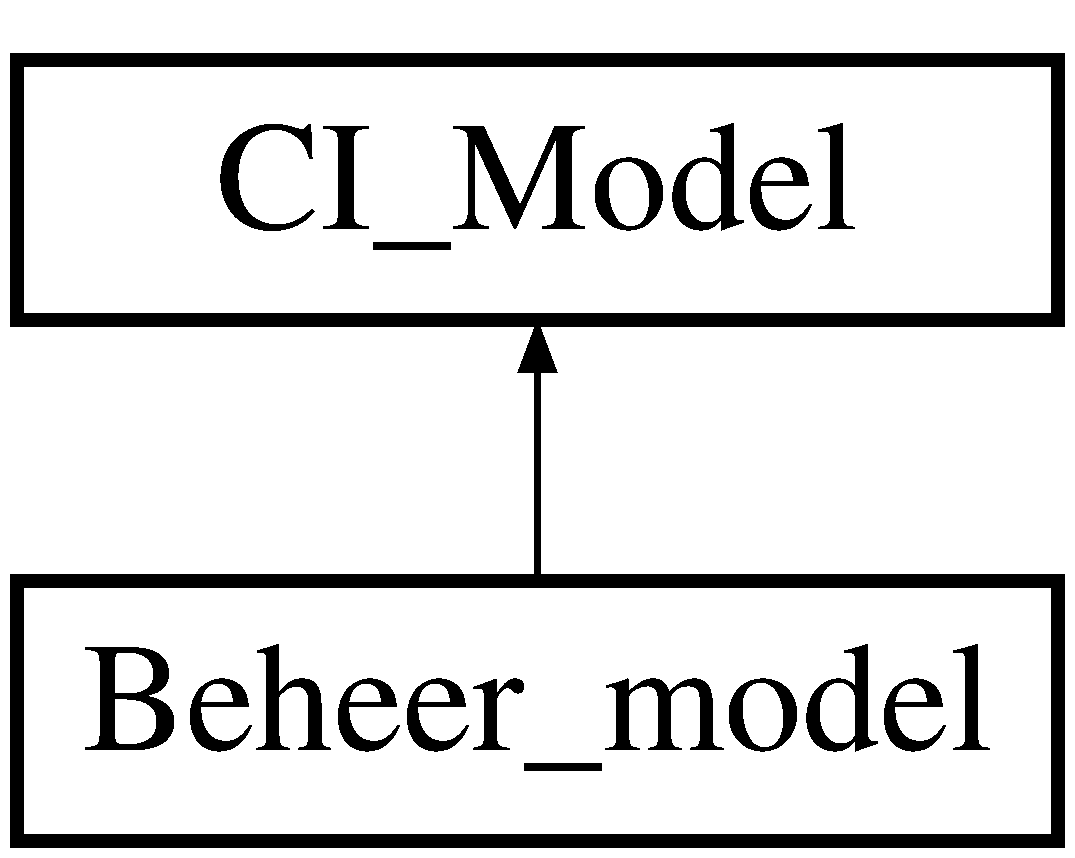
\includegraphics[height=2.000000cm]{class_beheer__model}
\end{center}
\end{figure}
\subsection*{Public Member Functions}
\begin{DoxyCompactItemize}
\item 
\mbox{\Hypertarget{class_beheer__model_aff0ccaed0f67602297ac11a535a53af9}\label{class_beheer__model_aff0ccaed0f67602297ac11a535a53af9}} 
{\bfseries login} (\$username, \$pass)
\item 
\mbox{\Hypertarget{class_beheer__model_ae1918ad227881de34ca871dca896a623}\label{class_beheer__model_ae1918ad227881de34ca871dca896a623}} 
{\bfseries login\+\_\+by\+Id} (\$id, \$pass)
\item 
\mbox{\Hypertarget{class_beheer__model_aba0d5b303383fb5b1fabb5fd01cd3800}\label{class_beheer__model_aba0d5b303383fb5b1fabb5fd01cd3800}} 
{\bfseries get\+All} ()
\item 
\mbox{\Hypertarget{class_beheer__model_a98d28a4d9a29d40c5a8aa0176f19a919}\label{class_beheer__model_a98d28a4d9a29d40c5a8aa0176f19a919}} 
{\bfseries get\+\_\+by\+Id} (\$id)
\item 
\mbox{\Hypertarget{class_beheer__model_a9b26d258cdfbbf0025a56dbe2f0088b0}\label{class_beheer__model_a9b26d258cdfbbf0025a56dbe2f0088b0}} 
{\bfseries update} (\$admin)
\item 
\mbox{\Hypertarget{class_beheer__model_a9a6cdec5d258d2b51d1a7619909b2a90}\label{class_beheer__model_a9a6cdec5d258d2b51d1a7619909b2a90}} 
{\bfseries add} (\$admin)
\item 
\mbox{\Hypertarget{class_beheer__model_a2f8258add505482d7f00ea26493a5723}\label{class_beheer__model_a2f8258add505482d7f00ea26493a5723}} 
{\bfseries delete} (\$id)
\end{DoxyCompactItemize}


The documentation for this class was generated from the following file\+:\begin{DoxyCompactItemize}
\item 
application/models/Beheer\+\_\+model.\+php\end{DoxyCompactItemize}

\hypertarget{classcsv__model}{}\section{csv\+\_\+model Class Reference}
\label{classcsv__model}\index{csv\+\_\+model@{csv\+\_\+model}}
Inheritance diagram for csv\+\_\+model\+:\begin{figure}[H]
\begin{center}
\leavevmode
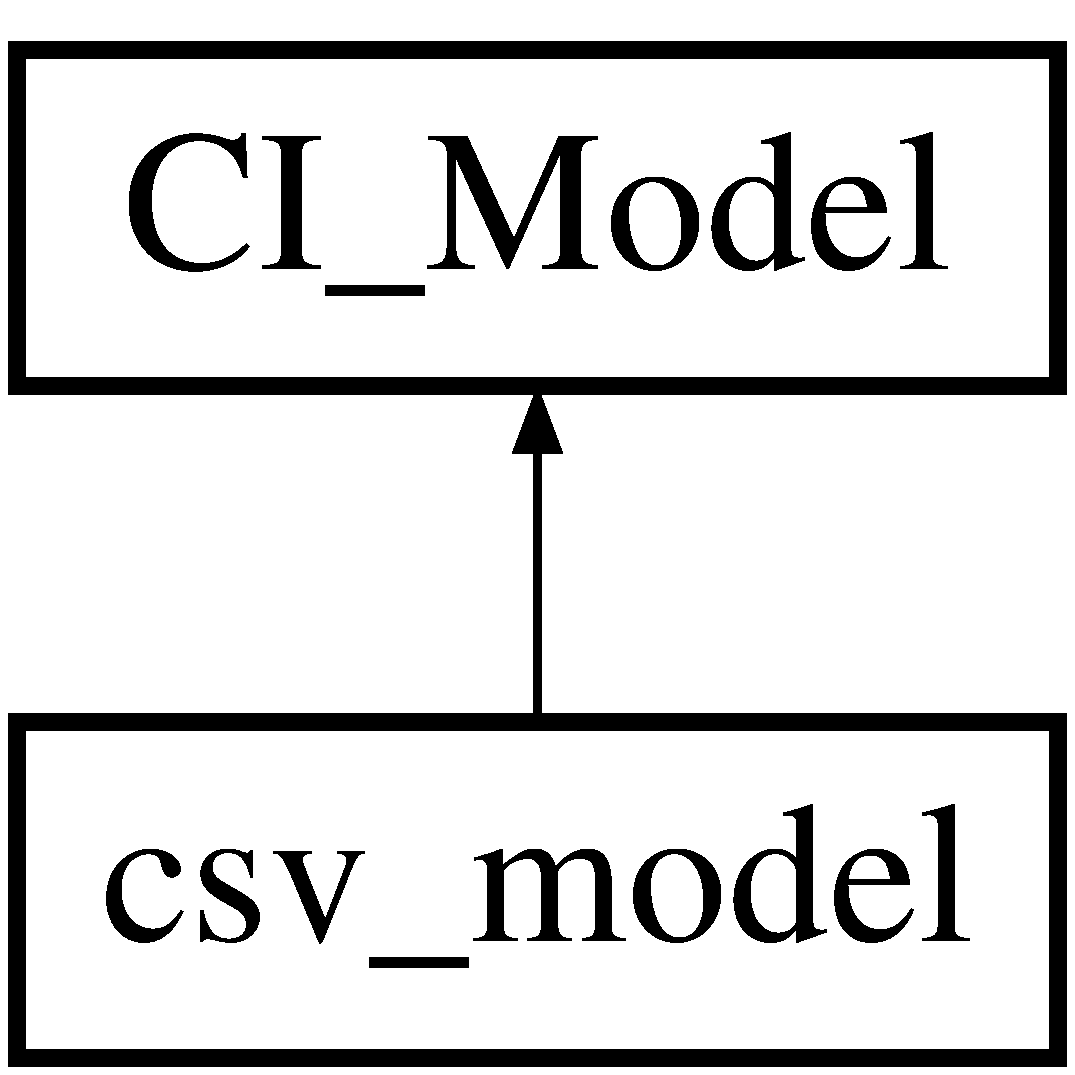
\includegraphics[height=2.000000cm]{classcsv__model}
\end{center}
\end{figure}
\subsection*{Public Member Functions}
\begin{DoxyCompactItemize}
\item 
\mbox{\hyperlink{classcsv__model_a095c5d389db211932136b53f25f39685}{\+\_\+\+\_\+construct}} ()
\item 
\mbox{\hyperlink{classcsv__model_a0982b277c56508192bc564cd095e9541}{readpersonen}} (\$soort)
\begin{DoxyCompactList}\small\item\em lees een csv bestand in om een persoon toe te voegen aan de database met personen\+\_\+model \end{DoxyCompactList}\end{DoxyCompactItemize}


\subsection{Constructor \& Destructor Documentation}
\mbox{\Hypertarget{classcsv__model_a095c5d389db211932136b53f25f39685}\label{classcsv__model_a095c5d389db211932136b53f25f39685}} 
\index{csv\+\_\+model@{csv\+\_\+model}!\+\_\+\+\_\+construct@{\+\_\+\+\_\+construct}}
\index{\+\_\+\+\_\+construct@{\+\_\+\+\_\+construct}!csv\+\_\+model@{csv\+\_\+model}}
\subsubsection{\texorpdfstring{\+\_\+\+\_\+construct()}{\_\_construct()}}
{\footnotesize\ttfamily \+\_\+\+\_\+construct (\begin{DoxyParamCaption}{ }\end{DoxyParamCaption})}



\subsection{Member Function Documentation}
\mbox{\Hypertarget{classcsv__model_a0982b277c56508192bc564cd095e9541}\label{classcsv__model_a0982b277c56508192bc564cd095e9541}} 
\index{csv\+\_\+model@{csv\+\_\+model}!readpersonen@{readpersonen}}
\index{readpersonen@{readpersonen}!csv\+\_\+model@{csv\+\_\+model}}
\subsubsection{\texorpdfstring{readpersonen()}{readpersonen()}}
{\footnotesize\ttfamily readpersonen (\begin{DoxyParamCaption}\item[{}]{\$soort }\end{DoxyParamCaption})}



lees een csv bestand in om een persoon toe te voegen aan de database met personen\+\_\+model 

lees de csv file

pak de index van e headers van de csv file op de 1ste lijn

lees de 1ste lijn van de file

slaag de index van de headers op voor later

lees lijn per lijn de personen uit ~\newline
~\newline
~\newline
 kijk of elk element is ingevuld zoniet wordt een null opgelagen in het veld ~\newline
~\newline
 voeg de gelezen persoon toe

einde csv file, stop de functie 

The documentation for this class was generated from the following file\+:\begin{DoxyCompactItemize}
\item 
application/models/\mbox{\hyperlink{_c_s_v__model_8php}{C\+S\+V\+\_\+model.\+php}}\end{DoxyCompactItemize}

\hypertarget{class_deelnemer}{}\section{Deelnemer Class Reference}
\label{class_deelnemer}\index{Deelnemer@{Deelnemer}}


Constructor voor deelnemer functionaliteiten.  


Inheritance diagram for Deelnemer\+:\begin{figure}[H]
\begin{center}
\leavevmode
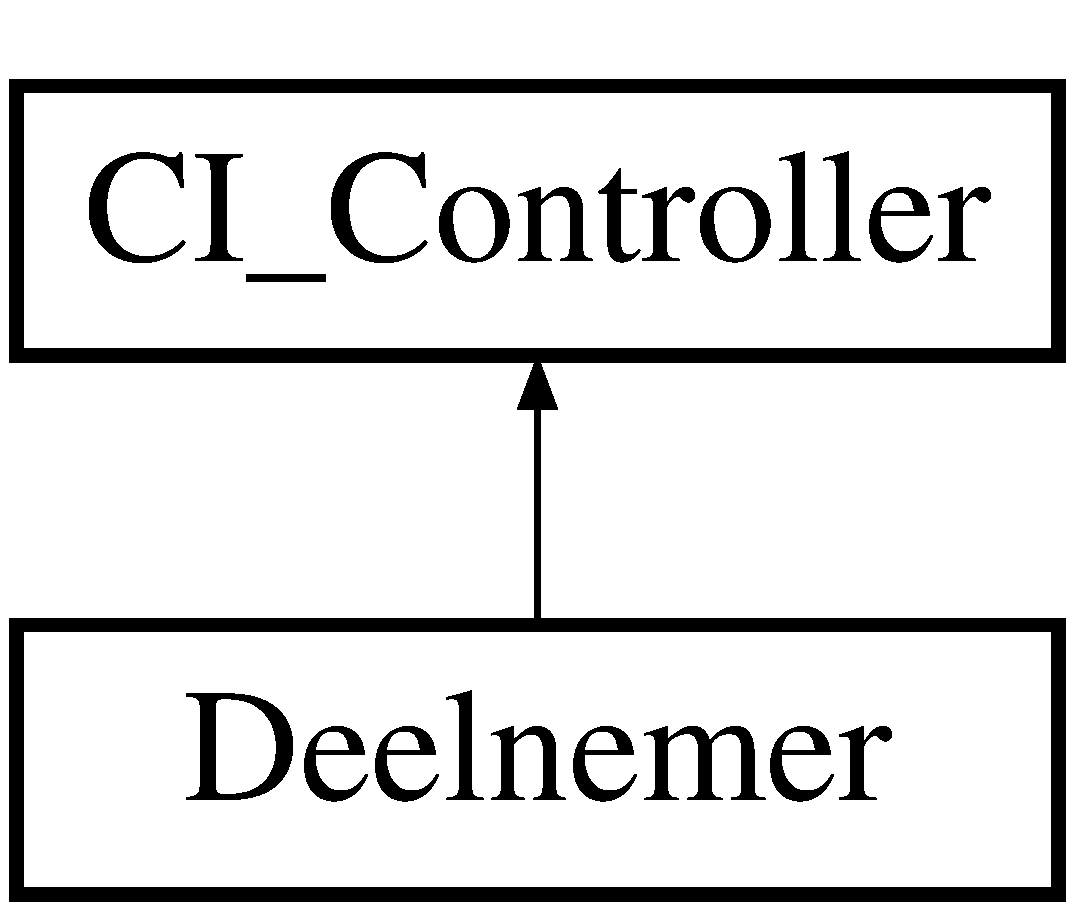
\includegraphics[height=2.000000cm]{class_deelnemer}
\end{center}
\end{figure}
\subsection*{Public Member Functions}
\begin{DoxyCompactItemize}
\item 
\mbox{\hyperlink{class_deelnemer_a095c5d389db211932136b53f25f39685}{\+\_\+\+\_\+construct}} ()
\item 
\mbox{\hyperlink{class_deelnemer_a35f5125b52883ea70807c42282f60b54}{dash}} (\$view=null, \$extras=null)
\item 
\mbox{\hyperlink{class_deelnemer_a082405d89acd6835c3a7c7a08a7adbab}{logout}} ()
\item 
\mbox{\hyperlink{class_deelnemer_a4ad528eb297f8dc0084b986f58fe2d2c}{vrijwilligertoevoegen}} ()
\end{DoxyCompactItemize}


\subsection{Detailed Description}
Constructor voor deelnemer functionaliteiten. 

\subsection{Constructor \& Destructor Documentation}
\mbox{\Hypertarget{class_deelnemer_a095c5d389db211932136b53f25f39685}\label{class_deelnemer_a095c5d389db211932136b53f25f39685}} 
\index{Deelnemer@{Deelnemer}!\+\_\+\+\_\+construct@{\+\_\+\+\_\+construct}}
\index{\+\_\+\+\_\+construct@{\+\_\+\+\_\+construct}!Deelnemer@{Deelnemer}}
\subsubsection{\texorpdfstring{\+\_\+\+\_\+construct()}{\_\_construct()}}
{\footnotesize\ttfamily \+\_\+\+\_\+construct (\begin{DoxyParamCaption}{ }\end{DoxyParamCaption})}

Default Contstructor 

\subsection{Member Function Documentation}
\mbox{\Hypertarget{class_deelnemer_a35f5125b52883ea70807c42282f60b54}\label{class_deelnemer_a35f5125b52883ea70807c42282f60b54}} 
\index{Deelnemer@{Deelnemer}!dash@{dash}}
\index{dash@{dash}!Deelnemer@{Deelnemer}}
\subsubsection{\texorpdfstring{dash()}{dash()}}
{\footnotesize\ttfamily dash (\begin{DoxyParamCaption}\item[{}]{\$view = {\ttfamily null},  }\item[{}]{\$extras = {\ttfamily null} }\end{DoxyParamCaption})}

Container voor alle dashbord schermen van deelnemer 
\begin{DoxyParams}[1]{Parameters}
string & {\em \$view} & Scherm dat opgeroepen word in het dashbord van administrator \\
\hline
string & {\em \$extras} & Optionele parameters \\
\hline
\end{DoxyParams}
\mbox{\Hypertarget{class_deelnemer_a082405d89acd6835c3a7c7a08a7adbab}\label{class_deelnemer_a082405d89acd6835c3a7c7a08a7adbab}} 
\index{Deelnemer@{Deelnemer}!logout@{logout}}
\index{logout@{logout}!Deelnemer@{Deelnemer}}
\subsubsection{\texorpdfstring{logout()}{logout()}}
{\footnotesize\ttfamily logout (\begin{DoxyParamCaption}{ }\end{DoxyParamCaption})}

Meld administrator af \mbox{\Hypertarget{class_deelnemer_a4ad528eb297f8dc0084b986f58fe2d2c}\label{class_deelnemer_a4ad528eb297f8dc0084b986f58fe2d2c}} 
\index{Deelnemer@{Deelnemer}!vrijwilligertoevoegen@{vrijwilligertoevoegen}}
\index{vrijwilligertoevoegen@{vrijwilligertoevoegen}!Deelnemer@{Deelnemer}}
\subsubsection{\texorpdfstring{vrijwilligertoevoegen()}{vrijwilligertoevoegen()}}
{\footnotesize\ttfamily vrijwilligertoevoegen (\begin{DoxyParamCaption}{ }\end{DoxyParamCaption})}



The documentation for this class was generated from the following file\+:\begin{DoxyCompactItemize}
\item 
application/controllers/\mbox{\hyperlink{_deelnemer_8php}{Deelnemer.\+php}}\end{DoxyCompactItemize}

\hypertarget{class_jaargang}{}\section{Jaargang Class Reference}
\label{class_jaargang}\index{Jaargang@{Jaargang}}
Inheritance diagram for Jaargang\+:\begin{figure}[H]
\begin{center}
\leavevmode
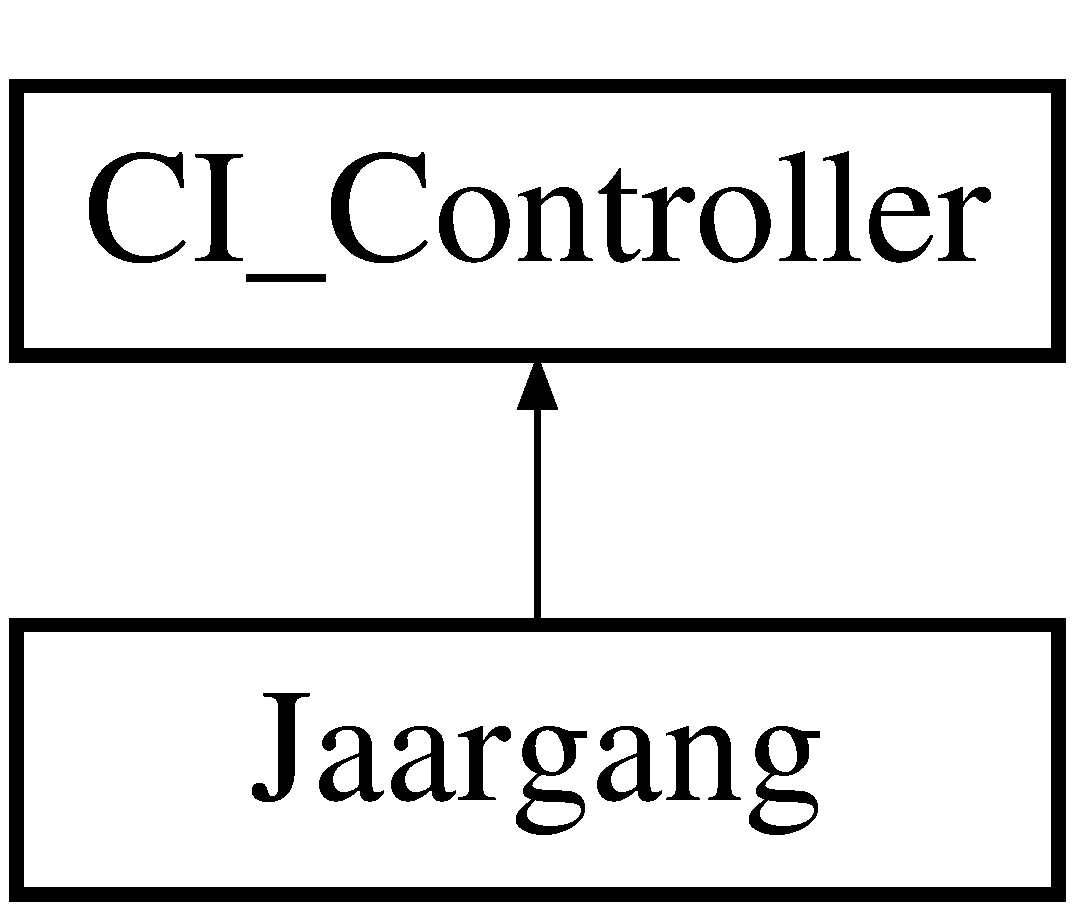
\includegraphics[height=2.000000cm]{class_jaargang}
\end{center}
\end{figure}
\subsection*{Public Member Functions}
\begin{DoxyCompactItemize}
\item 
\mbox{\Hypertarget{class_jaargang_a842e4774e3b3601a005b995c02f7e883}\label{class_jaargang_a842e4774e3b3601a005b995c02f7e883}} 
{\bfseries update} ()
\item 
\mbox{\Hypertarget{class_jaargang_a96b12cad9ede16ef3e87c74cf77b894b}\label{class_jaargang_a96b12cad9ede16ef3e87c74cf77b894b}} 
{\bfseries end} (\$id)
\end{DoxyCompactItemize}


The documentation for this class was generated from the following file\+:\begin{DoxyCompactItemize}
\item 
application/controllers/Jaargang.\+php\end{DoxyCompactItemize}

\hypertarget{class_jaargang__model}{}\section{Jaargang\+\_\+model Class Reference}
\label{class_jaargang__model}\index{Jaargang\+\_\+model@{Jaargang\+\_\+model}}
Inheritance diagram for Jaargang\+\_\+model\+:\begin{figure}[H]
\begin{center}
\leavevmode
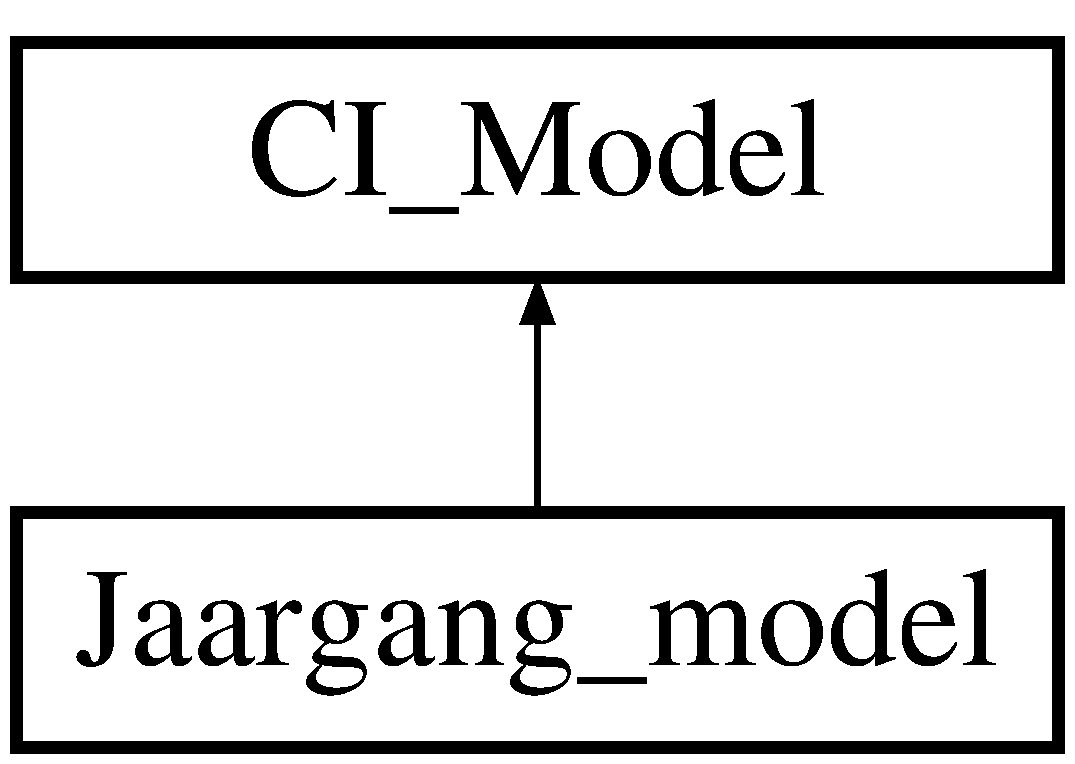
\includegraphics[height=2.000000cm]{class_jaargang__model}
\end{center}
\end{figure}
\subsection*{Public Member Functions}
\begin{DoxyCompactItemize}
\item 
\mbox{\hyperlink{class_jaargang__model_a8556a042a80cea1a12445d8389c2e019}{\+\_\+\+\_\+construct}} ()
\item 
\mbox{\hyperlink{class_jaargang__model_a10cf39c5710240aec9aad633253e3048}{get\+\_\+by\+Id}} (\$id)
\item 
\mbox{\hyperlink{class_jaargang__model_a25674521a1a6a191c6cc77e524e5b8f5}{get\+All}} ()
\item 
\mbox{\hyperlink{class_jaargang__model_ab77c5c935c05d5bc08630111f3f0273f}{get\+All\+By\+Jaargang}} ()
\item 
\mbox{\hyperlink{class_jaargang__model_aba56cc05b3878d487d723edfe4464803}{get\+Allby\+Begin\+Tijdstip}} ()
\item 
\mbox{\hyperlink{class_jaargang__model_a56a8c0bc2beb0dca5ab28ca8d019d64e}{end}} (\$jaargang)
\item 
\mbox{\hyperlink{class_jaargang__model_a4e55f912a50eea5f66669fec3ae11f6d}{get\+Actief}} ()
\item 
\mbox{\hyperlink{class_jaargang__model_a18ab753f7cf3d830f513979cff49e2b8}{update}} (\$jaargang)
\item 
\mbox{\hyperlink{class_jaargang__model_a726ba676b9f198c0bf77191a66262421}{add}} (\$jaargang)
\item 
\mbox{\hyperlink{class_jaargang__model_a99ab50dc52b431939edc5db85b857bc6}{get\+With\+Keuzemogelijkheid\+With\+Opties\+\_\+by\+Id}} (\$id)
\end{DoxyCompactItemize}


\subsection{Constructor \& Destructor Documentation}
\mbox{\Hypertarget{class_jaargang__model_a8556a042a80cea1a12445d8389c2e019}\label{class_jaargang__model_a8556a042a80cea1a12445d8389c2e019}} 
\index{Jaargang\+\_\+model@{Jaargang\+\_\+model}!\+\_\+\+\_\+construct@{\+\_\+\+\_\+construct}}
\index{\+\_\+\+\_\+construct@{\+\_\+\+\_\+construct}!Jaargang\+\_\+model@{Jaargang\+\_\+model}}
\subsubsection{\texorpdfstring{\+\_\+\+\_\+construct()}{\_\_construct()}}
{\footnotesize\ttfamily Jaargang\+\_\+model\+::\+\_\+\+\_\+construct (\begin{DoxyParamCaption}{ }\end{DoxyParamCaption})}

Default Constructor 

\subsection{Member Function Documentation}
\mbox{\Hypertarget{class_jaargang__model_a726ba676b9f198c0bf77191a66262421}\label{class_jaargang__model_a726ba676b9f198c0bf77191a66262421}} 
\index{Jaargang\+\_\+model@{Jaargang\+\_\+model}!add@{add}}
\index{add@{add}!Jaargang\+\_\+model@{Jaargang\+\_\+model}}
\subsubsection{\texorpdfstring{add()}{add()}}
{\footnotesize\ttfamily Jaargang\+\_\+model\+::add (\begin{DoxyParamCaption}\item[{}]{\$jaargang }\end{DoxyParamCaption})}

Voeg jaargang toe 
\begin{DoxyParams}[1]{Parameters}
\mbox{\hyperlink{class_jaargang}{Jaargang}} & {\em \$jaargang} & \mbox{\hyperlink{class_jaargang}{Jaargang}} Object dat toegevoegd word \\
\hline
\end{DoxyParams}

\begin{DoxyRetVals}{Return values}
{\em int} & Id van jaargang dat toegevoegd word \\
\hline
\end{DoxyRetVals}
\mbox{\Hypertarget{class_jaargang__model_a56a8c0bc2beb0dca5ab28ca8d019d64e}\label{class_jaargang__model_a56a8c0bc2beb0dca5ab28ca8d019d64e}} 
\index{Jaargang\+\_\+model@{Jaargang\+\_\+model}!end@{end}}
\index{end@{end}!Jaargang\+\_\+model@{Jaargang\+\_\+model}}
\subsubsection{\texorpdfstring{end()}{end()}}
{\footnotesize\ttfamily Jaargang\+\_\+model\+::end (\begin{DoxyParamCaption}\item[{}]{\$jaargang }\end{DoxyParamCaption})}

Beeindig jaargang 
\begin{DoxyParams}[1]{Parameters}
\mbox{\hyperlink{class_jaargang}{Jaargang}} & {\em \$jaargang} & \mbox{\hyperlink{class_jaargang}{Jaargang}} Object dat verwijderd moet worden \\
\hline
\end{DoxyParams}
\mbox{\Hypertarget{class_jaargang__model_a10cf39c5710240aec9aad633253e3048}\label{class_jaargang__model_a10cf39c5710240aec9aad633253e3048}} 
\index{Jaargang\+\_\+model@{Jaargang\+\_\+model}!get\+\_\+by\+Id@{get\+\_\+by\+Id}}
\index{get\+\_\+by\+Id@{get\+\_\+by\+Id}!Jaargang\+\_\+model@{Jaargang\+\_\+model}}
\subsubsection{\texorpdfstring{get\+\_\+by\+Id()}{get\_byId()}}
{\footnotesize\ttfamily Jaargang\+\_\+model\+::get\+\_\+by\+Id (\begin{DoxyParamCaption}\item[{}]{\$id }\end{DoxyParamCaption})}

Vraag informatie over jaargang 
\begin{DoxyParams}[1]{Parameters}
int & {\em \$id} & Id van jaargang \\
\hline
\end{DoxyParams}

\begin{DoxyRetVals}{Return values}
{\em \mbox{\hyperlink{class_jaargang}{Jaargang}}} & \mbox{\hyperlink{class_jaargang}{Jaargang}} \\
\hline
\end{DoxyRetVals}
\mbox{\Hypertarget{class_jaargang__model_a4e55f912a50eea5f66669fec3ae11f6d}\label{class_jaargang__model_a4e55f912a50eea5f66669fec3ae11f6d}} 
\index{Jaargang\+\_\+model@{Jaargang\+\_\+model}!get\+Actief@{get\+Actief}}
\index{get\+Actief@{get\+Actief}!Jaargang\+\_\+model@{Jaargang\+\_\+model}}
\subsubsection{\texorpdfstring{get\+Actief()}{getActief()}}
{\footnotesize\ttfamily Jaargang\+\_\+model\+::get\+Actief (\begin{DoxyParamCaption}{ }\end{DoxyParamCaption})}

Vraag actieve jaargang op 
\begin{DoxyRetVals}{Return values}
{\em \mbox{\hyperlink{class_jaargang}{Jaargang}}} & \mbox{\hyperlink{class_jaargang}{Jaargang}} \\
\hline
\end{DoxyRetVals}
\mbox{\Hypertarget{class_jaargang__model_a25674521a1a6a191c6cc77e524e5b8f5}\label{class_jaargang__model_a25674521a1a6a191c6cc77e524e5b8f5}} 
\index{Jaargang\+\_\+model@{Jaargang\+\_\+model}!get\+All@{get\+All}}
\index{get\+All@{get\+All}!Jaargang\+\_\+model@{Jaargang\+\_\+model}}
\subsubsection{\texorpdfstring{get\+All()}{getAll()}}
{\footnotesize\ttfamily Jaargang\+\_\+model\+::get\+All (\begin{DoxyParamCaption}{ }\end{DoxyParamCaption})}

Vraag alle jaargangen op 
\begin{DoxyRetVals}{Return values}
{\em List$<$\+Jaargang$>$} & \mbox{\hyperlink{class_jaargang}{Jaargang}} lijst \\
\hline
\end{DoxyRetVals}
\mbox{\Hypertarget{class_jaargang__model_aba56cc05b3878d487d723edfe4464803}\label{class_jaargang__model_aba56cc05b3878d487d723edfe4464803}} 
\index{Jaargang\+\_\+model@{Jaargang\+\_\+model}!get\+Allby\+Begin\+Tijdstip@{get\+Allby\+Begin\+Tijdstip}}
\index{get\+Allby\+Begin\+Tijdstip@{get\+Allby\+Begin\+Tijdstip}!Jaargang\+\_\+model@{Jaargang\+\_\+model}}
\subsubsection{\texorpdfstring{get\+Allby\+Begin\+Tijdstip()}{getAllbyBeginTijdstip()}}
{\footnotesize\ttfamily Jaargang\+\_\+model\+::get\+Allby\+Begin\+Tijdstip (\begin{DoxyParamCaption}{ }\end{DoxyParamCaption})}

Vraag alle jaargangen op gesorteerd op begintijdstip 
\begin{DoxyRetVals}{Return values}
{\em List$<$\+Jaargang$>$} & \mbox{\hyperlink{class_jaargang}{Jaargang}} lijst \\
\hline
\end{DoxyRetVals}
\mbox{\Hypertarget{class_jaargang__model_ab77c5c935c05d5bc08630111f3f0273f}\label{class_jaargang__model_ab77c5c935c05d5bc08630111f3f0273f}} 
\index{Jaargang\+\_\+model@{Jaargang\+\_\+model}!get\+All\+By\+Jaargang@{get\+All\+By\+Jaargang}}
\index{get\+All\+By\+Jaargang@{get\+All\+By\+Jaargang}!Jaargang\+\_\+model@{Jaargang\+\_\+model}}
\subsubsection{\texorpdfstring{get\+All\+By\+Jaargang()}{getAllByJaargang()}}
{\footnotesize\ttfamily Jaargang\+\_\+model\+::get\+All\+By\+Jaargang (\begin{DoxyParamCaption}{ }\end{DoxyParamCaption})}

Vraag alle jaargangen op gesorteerd op naam 
\begin{DoxyRetVals}{Return values}
{\em List$<$\+Jaargang$>$} & \mbox{\hyperlink{class_jaargang}{Jaargang}} lijst \\
\hline
\end{DoxyRetVals}
\mbox{\Hypertarget{class_jaargang__model_a99ab50dc52b431939edc5db85b857bc6}\label{class_jaargang__model_a99ab50dc52b431939edc5db85b857bc6}} 
\index{Jaargang\+\_\+model@{Jaargang\+\_\+model}!get\+With\+Keuzemogelijkheid\+With\+Opties\+\_\+by\+Id@{get\+With\+Keuzemogelijkheid\+With\+Opties\+\_\+by\+Id}}
\index{get\+With\+Keuzemogelijkheid\+With\+Opties\+\_\+by\+Id@{get\+With\+Keuzemogelijkheid\+With\+Opties\+\_\+by\+Id}!Jaargang\+\_\+model@{Jaargang\+\_\+model}}
\subsubsection{\texorpdfstring{get\+With\+Keuzemogelijkheid\+With\+Opties\+\_\+by\+Id()}{getWithKeuzemogelijkheidWithOpties\_byId()}}
{\footnotesize\ttfamily Jaargang\+\_\+model\+::get\+With\+Keuzemogelijkheid\+With\+Opties\+\_\+by\+Id (\begin{DoxyParamCaption}\item[{}]{\$id }\end{DoxyParamCaption})}

Vraag jaargang op met keuzemogelijkheden 
\begin{DoxyParams}[1]{Parameters}
int & {\em \$id} & Id van jaargang \\
\hline
\end{DoxyParams}

\begin{DoxyRetVals}{Return values}
{\em List$<$\+Jaargang,Keuzemogelijkheid$>$} & Lijst met Objects die \mbox{\hyperlink{class_jaargang}{Jaargang}} met \mbox{\hyperlink{class_keuzemogelijkheid}{Keuzemogelijkheid}} bevatten \\
\hline
\end{DoxyRetVals}
\mbox{\Hypertarget{class_jaargang__model_a18ab753f7cf3d830f513979cff49e2b8}\label{class_jaargang__model_a18ab753f7cf3d830f513979cff49e2b8}} 
\index{Jaargang\+\_\+model@{Jaargang\+\_\+model}!update@{update}}
\index{update@{update}!Jaargang\+\_\+model@{Jaargang\+\_\+model}}
\subsubsection{\texorpdfstring{update()}{update()}}
{\footnotesize\ttfamily Jaargang\+\_\+model\+::update (\begin{DoxyParamCaption}\item[{}]{\$jaargang }\end{DoxyParamCaption})}

Update jaargang 
\begin{DoxyParams}[1]{Parameters}
\mbox{\hyperlink{class_jaargang}{Jaargang}} & {\em \$jaargang} & \mbox{\hyperlink{class_jaargang}{Jaargang}} Object dat aangepast word \\
\hline
\end{DoxyParams}


The documentation for this class was generated from the following file\+:\begin{DoxyCompactItemize}
\item 
E\+:/\+D\+R\+I\+V\+E/\+C\+O\+L\+L\+E\+G\+E/\+T\+M/\+P0202/\+K\+P0201/\+R\+E\+P\+O/application/models/Jaargang\+\_\+model.\+php\end{DoxyCompactItemize}

\hypertarget{class_keuzemogelijkheid}{}\section{Keuzemogelijkheid Class Reference}
\label{class_keuzemogelijkheid}\index{Keuzemogelijkheid@{Keuzemogelijkheid}}


Controller voor keuzemogelijkheidfunctionaliteiten.  


Inheritance diagram for Keuzemogelijkheid\+:\begin{figure}[H]
\begin{center}
\leavevmode
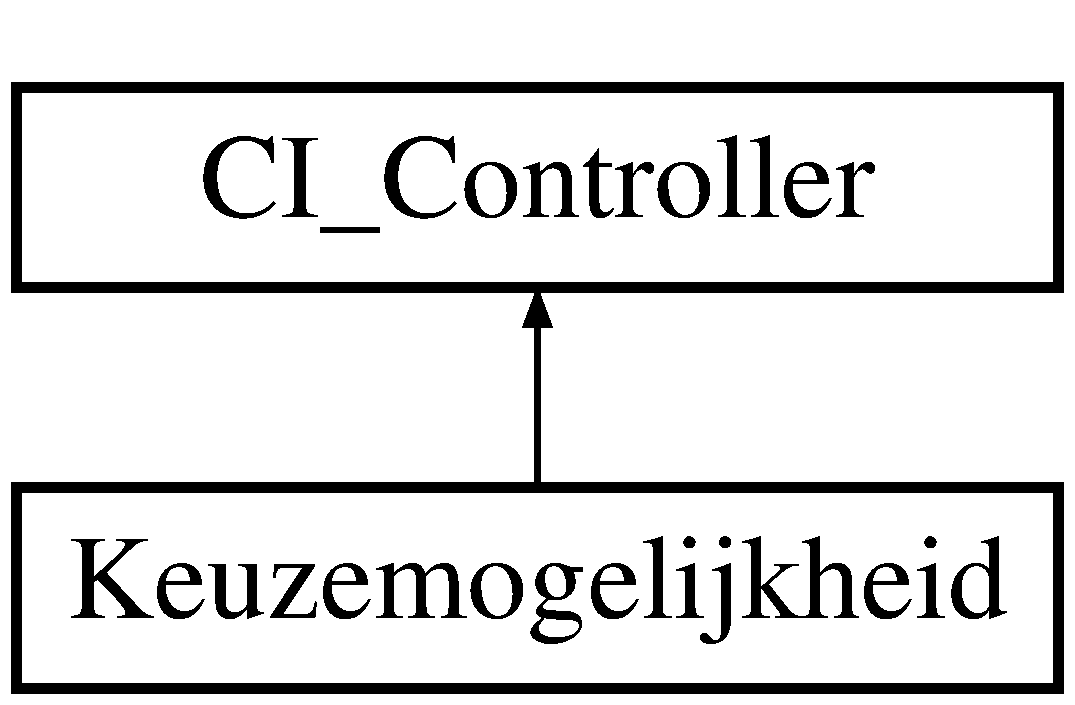
\includegraphics[height=2.000000cm]{class_keuzemogelijkheid}
\end{center}
\end{figure}
\subsection*{Public Member Functions}
\begin{DoxyCompactItemize}
\item 
\mbox{\hyperlink{class_keuzemogelijkheid_a11bdb9d39ff85f7e9a5a7f4f13eca123}{\+\_\+\+\_\+construct}} ()
\item 
\mbox{\hyperlink{class_keuzemogelijkheid_a507c36e7d7fd35a2a080524fce31ec4d}{get}} (\$id)
\item 
\mbox{\hyperlink{class_keuzemogelijkheid_ae621c2f2cc768da82291345a301f746a}{update}} ()
\item 
\mbox{\hyperlink{class_keuzemogelijkheid_a569638d382493486135eeea9b7d1cca5}{delete}} (\$id)
\end{DoxyCompactItemize}


\subsection{Detailed Description}
Controller voor keuzemogelijkheidfunctionaliteiten. 

\subsection{Constructor \& Destructor Documentation}
\mbox{\Hypertarget{class_keuzemogelijkheid_a11bdb9d39ff85f7e9a5a7f4f13eca123}\label{class_keuzemogelijkheid_a11bdb9d39ff85f7e9a5a7f4f13eca123}} 
\index{Keuzemogelijkheid@{Keuzemogelijkheid}!\+\_\+\+\_\+construct@{\+\_\+\+\_\+construct}}
\index{\+\_\+\+\_\+construct@{\+\_\+\+\_\+construct}!Keuzemogelijkheid@{Keuzemogelijkheid}}
\subsubsection{\texorpdfstring{\+\_\+\+\_\+construct()}{\_\_construct()}}
{\footnotesize\ttfamily Keuzemogelijkheid\+::\+\_\+\+\_\+construct (\begin{DoxyParamCaption}{ }\end{DoxyParamCaption})}

Default Constructor

\subsection{Member Function Documentation}
\mbox{\Hypertarget{class_keuzemogelijkheid_a569638d382493486135eeea9b7d1cca5}\label{class_keuzemogelijkheid_a569638d382493486135eeea9b7d1cca5}} 
\index{Keuzemogelijkheid@{Keuzemogelijkheid}!delete@{delete}}
\index{delete@{delete}!Keuzemogelijkheid@{Keuzemogelijkheid}}
\subsubsection{\texorpdfstring{delete()}{delete()}}
{\footnotesize\ttfamily Keuzemogelijkheid\+::delete (\begin{DoxyParamCaption}\item[{}]{\$id }\end{DoxyParamCaption})}

Verwijder keuzemogelijkheid 
\begin{DoxyParams}[1]{Parameters}
int & {\em \$id} & Id van keuzemogelijkheid \\
\hline
\end{DoxyParams}
\mbox{\Hypertarget{class_keuzemogelijkheid_a507c36e7d7fd35a2a080524fce31ec4d}\label{class_keuzemogelijkheid_a507c36e7d7fd35a2a080524fce31ec4d}} 
\index{Keuzemogelijkheid@{Keuzemogelijkheid}!get@{get}}
\index{get@{get}!Keuzemogelijkheid@{Keuzemogelijkheid}}
\subsubsection{\texorpdfstring{get()}{get()}}
{\footnotesize\ttfamily Keuzemogelijkheid\+::get (\begin{DoxyParamCaption}\item[{}]{\$id }\end{DoxyParamCaption})}

Vraag keuzemogelijkheid op 
\begin{DoxyParams}[1]{Parameters}
int & {\em \$id} & Id van keuzemogelijkheid \\
\hline
\end{DoxyParams}
\mbox{\Hypertarget{class_keuzemogelijkheid_ae621c2f2cc768da82291345a301f746a}\label{class_keuzemogelijkheid_ae621c2f2cc768da82291345a301f746a}} 
\index{Keuzemogelijkheid@{Keuzemogelijkheid}!update@{update}}
\index{update@{update}!Keuzemogelijkheid@{Keuzemogelijkheid}}
\subsubsection{\texorpdfstring{update()}{update()}}
{\footnotesize\ttfamily Keuzemogelijkheid\+::update (\begin{DoxyParamCaption}{ }\end{DoxyParamCaption})}

Pas keuzemogelijkheid aan 

The documentation for this class was generated from the following file\+:\begin{DoxyCompactItemize}
\item 
application/controllers/Keuzemogelijkheid.\+php\end{DoxyCompactItemize}

\hypertarget{class_keuzemogelijkheid___model}{}\section{Keuzemogelijkheid\+\_\+\+Model Class Reference}
\label{class_keuzemogelijkheid___model}\index{Keuzemogelijkheid\+\_\+\+Model@{Keuzemogelijkheid\+\_\+\+Model}}
Inheritance diagram for Keuzemogelijkheid\+\_\+\+Model\+:\begin{figure}[H]
\begin{center}
\leavevmode
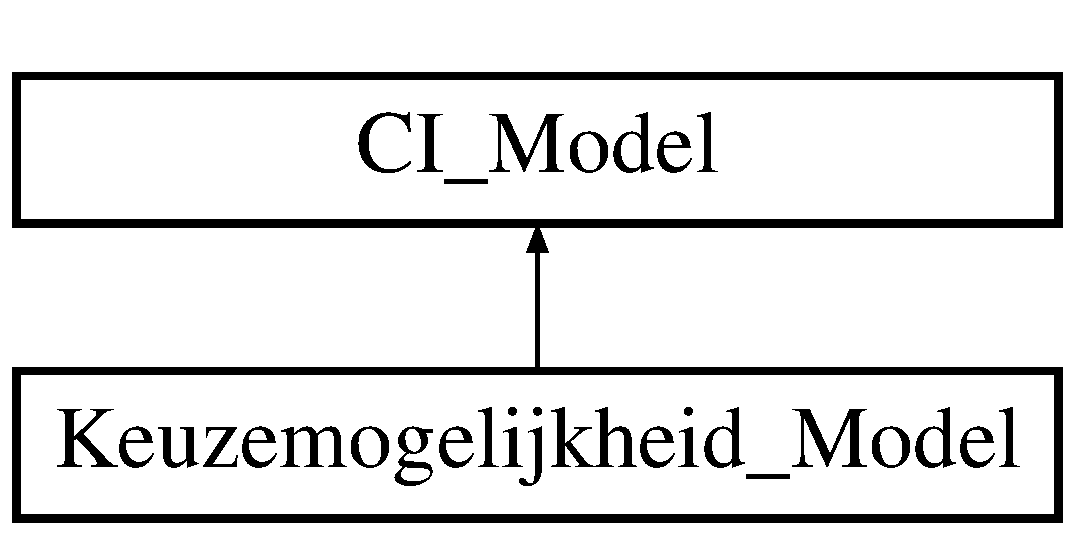
\includegraphics[height=2.000000cm]{class_keuzemogelijkheid___model}
\end{center}
\end{figure}
\subsection*{Public Member Functions}
\begin{DoxyCompactItemize}
\item 
\mbox{\Hypertarget{class_keuzemogelijkheid___model_a98d28a4d9a29d40c5a8aa0176f19a919}\label{class_keuzemogelijkheid___model_a98d28a4d9a29d40c5a8aa0176f19a919}} 
{\bfseries get\+\_\+by\+Id} (\$id)
\item 
\mbox{\Hypertarget{class_keuzemogelijkheid___model_a2b035b1ffd1cbe651b35bb3e53d72c09}\label{class_keuzemogelijkheid___model_a2b035b1ffd1cbe651b35bb3e53d72c09}} 
{\bfseries get\+All\+By\+Naam} ()
\item 
\mbox{\Hypertarget{class_keuzemogelijkheid___model_a2762d72d382c5c81da0d0830d5d91805}\label{class_keuzemogelijkheid___model_a2762d72d382c5c81da0d0830d5d91805}} 
{\bfseries get\+All\+By\+Naam\+With\+Keuze\+Opties} ()
\item 
\mbox{\Hypertarget{class_keuzemogelijkheid___model_aa7334b3aaafdacd36e91e44a83e668c3}\label{class_keuzemogelijkheid___model_aa7334b3aaafdacd36e91e44a83e668c3}} 
{\bfseries get\+All\+\_\+by\+Jaargang\+Id} (\$id)
\item 
\mbox{\Hypertarget{class_keuzemogelijkheid___model_afee956c75c2fe9966783b18602ace19a}\label{class_keuzemogelijkheid___model_afee956c75c2fe9966783b18602ace19a}} 
{\bfseries get\+All\+With\+Keuze\+Opties\+\_\+by\+Jaargang\+Id} (\$id)
\item 
\mbox{\Hypertarget{class_keuzemogelijkheid___model_a933a162ba87e58d4cc7eb781fd571a7a}\label{class_keuzemogelijkheid___model_a933a162ba87e58d4cc7eb781fd571a7a}} 
{\bfseries update} (\$keuzemogelijkheid)
\item 
\mbox{\Hypertarget{class_keuzemogelijkheid___model_ab3ea46c3ea11cbb463eb98238e38c580}\label{class_keuzemogelijkheid___model_ab3ea46c3ea11cbb463eb98238e38c580}} 
{\bfseries add} (\$keuzemogelijkheid)
\item 
\mbox{\Hypertarget{class_keuzemogelijkheid___model_a2f8258add505482d7f00ea26493a5723}\label{class_keuzemogelijkheid___model_a2f8258add505482d7f00ea26493a5723}} 
{\bfseries delete} (\$id)
\end{DoxyCompactItemize}


The documentation for this class was generated from the following file\+:\begin{DoxyCompactItemize}
\item 
application/models/Keuzemogelijkheid\+\_\+model.\+php\end{DoxyCompactItemize}

\hypertarget{class_keuzeoptie}{}\section{Keuzeoptie Class Reference}
\label{class_keuzeoptie}\index{Keuzeoptie@{Keuzeoptie}}
Inheritance diagram for Keuzeoptie\+:\begin{figure}[H]
\begin{center}
\leavevmode
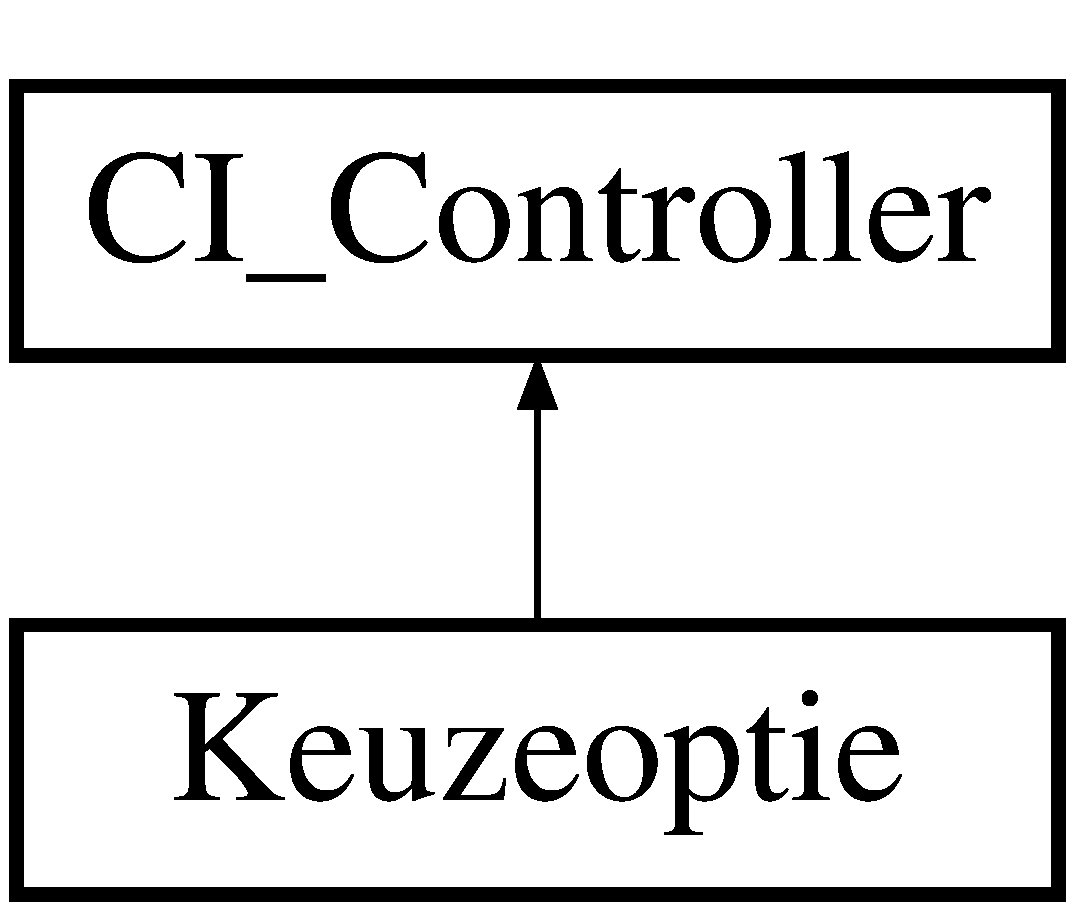
\includegraphics[height=2.000000cm]{class_keuzeoptie}
\end{center}
\end{figure}
\subsection*{Public Member Functions}
\begin{DoxyCompactItemize}
\item 
\mbox{\hyperlink{class_keuzeoptie_a095c5d389db211932136b53f25f39685}{\+\_\+\+\_\+construct}} ()
\item 
\mbox{\hyperlink{class_keuzeoptie_a50e3bfb586b2f42932a6a93f3fbb0828}{get}} (\$id)
\item 
\mbox{\hyperlink{class_keuzeoptie_a842e4774e3b3601a005b995c02f7e883}{update}} ()
\begin{DoxyCompactList}\small\item\em =================================================================================================== /\+G\+R\+E\+IF M\+A\+T\+T\+H\+I\+AS \end{DoxyCompactList}\item 
\mbox{\hyperlink{class_keuzeoptie_a2f8258add505482d7f00ea26493a5723}{delete}} (\$id)
\begin{DoxyCompactList}\small\item\em Functie om keuzeopties te verwijderen. \end{DoxyCompactList}\end{DoxyCompactItemize}


\subsection{Constructor \& Destructor Documentation}
\mbox{\Hypertarget{class_keuzeoptie_a095c5d389db211932136b53f25f39685}\label{class_keuzeoptie_a095c5d389db211932136b53f25f39685}} 
\index{Keuzeoptie@{Keuzeoptie}!\+\_\+\+\_\+construct@{\+\_\+\+\_\+construct}}
\index{\+\_\+\+\_\+construct@{\+\_\+\+\_\+construct}!Keuzeoptie@{Keuzeoptie}}
\subsubsection{\texorpdfstring{\+\_\+\+\_\+construct()}{\_\_construct()}}
{\footnotesize\ttfamily \+\_\+\+\_\+construct (\begin{DoxyParamCaption}{ }\end{DoxyParamCaption})}

=================================================================================================== G\+R\+E\+IF M\+A\+T\+T\+H\+I\+AS Autoload ~\newline
~\newline
 Redirect to home if no session started

=================================================================================================== /\+G\+R\+E\+IF M\+A\+T\+T\+H\+I\+AS 

\subsection{Member Function Documentation}
\mbox{\Hypertarget{class_keuzeoptie_a2f8258add505482d7f00ea26493a5723}\label{class_keuzeoptie_a2f8258add505482d7f00ea26493a5723}} 
\index{Keuzeoptie@{Keuzeoptie}!delete@{delete}}
\index{delete@{delete}!Keuzeoptie@{Keuzeoptie}}
\subsubsection{\texorpdfstring{delete()}{delete()}}
{\footnotesize\ttfamily delete (\begin{DoxyParamCaption}\item[{}]{\$id }\end{DoxyParamCaption})}



Functie om keuzeopties te verwijderen. 

Redirect to keuzemogelijkheidbeheer \mbox{\Hypertarget{class_keuzeoptie_a50e3bfb586b2f42932a6a93f3fbb0828}\label{class_keuzeoptie_a50e3bfb586b2f42932a6a93f3fbb0828}} 
\index{Keuzeoptie@{Keuzeoptie}!get@{get}}
\index{get@{get}!Keuzeoptie@{Keuzeoptie}}
\subsubsection{\texorpdfstring{get()}{get()}}
{\footnotesize\ttfamily get (\begin{DoxyParamCaption}\item[{}]{\$id }\end{DoxyParamCaption})}

=================================================================================================== G\+R\+E\+IF M\+A\+T\+T\+H\+I\+AS Get \mbox{\hyperlink{class_keuzeoptie}{Keuzeoptie}} by Id Get data from db

Return data

Print in default api output view \mbox{\Hypertarget{class_keuzeoptie_a842e4774e3b3601a005b995c02f7e883}\label{class_keuzeoptie_a842e4774e3b3601a005b995c02f7e883}} 
\index{Keuzeoptie@{Keuzeoptie}!update@{update}}
\index{update@{update}!Keuzeoptie@{Keuzeoptie}}
\subsubsection{\texorpdfstring{update()}{update()}}
{\footnotesize\ttfamily update (\begin{DoxyParamCaption}{ }\end{DoxyParamCaption})}



=================================================================================================== /\+G\+R\+E\+IF M\+A\+T\+T\+H\+I\+AS 

Functie voor het aanpassen en aanmaken van keuzeopties klasse \mbox{\hyperlink{class_keuzeoptie}{Keuzeoptie}} aanmaken en initialiseren

Model inladen

\mbox{\hyperlink{class_keuzeoptie}{Keuzeoptie}} toevoegen of aanpassen

\mbox{\hyperlink{class_keuzemogelijkheid}{Keuzemogelijkheid}} aanmaken om te kunnen redirecten naar de juiste pagina

Redirect naar keuzemogelijkheid pagina 

The documentation for this class was generated from the following file\+:\begin{DoxyCompactItemize}
\item 
application/controllers/\mbox{\hyperlink{_keuzeoptie_8php}{Keuzeoptie.\+php}}\end{DoxyCompactItemize}

\hypertarget{class_keuzeoptie___model}{}\section{Keuzeoptie\+\_\+\+Model Class Reference}
\label{class_keuzeoptie___model}\index{Keuzeoptie\+\_\+\+Model@{Keuzeoptie\+\_\+\+Model}}
Inheritance diagram for Keuzeoptie\+\_\+\+Model\+:\begin{figure}[H]
\begin{center}
\leavevmode
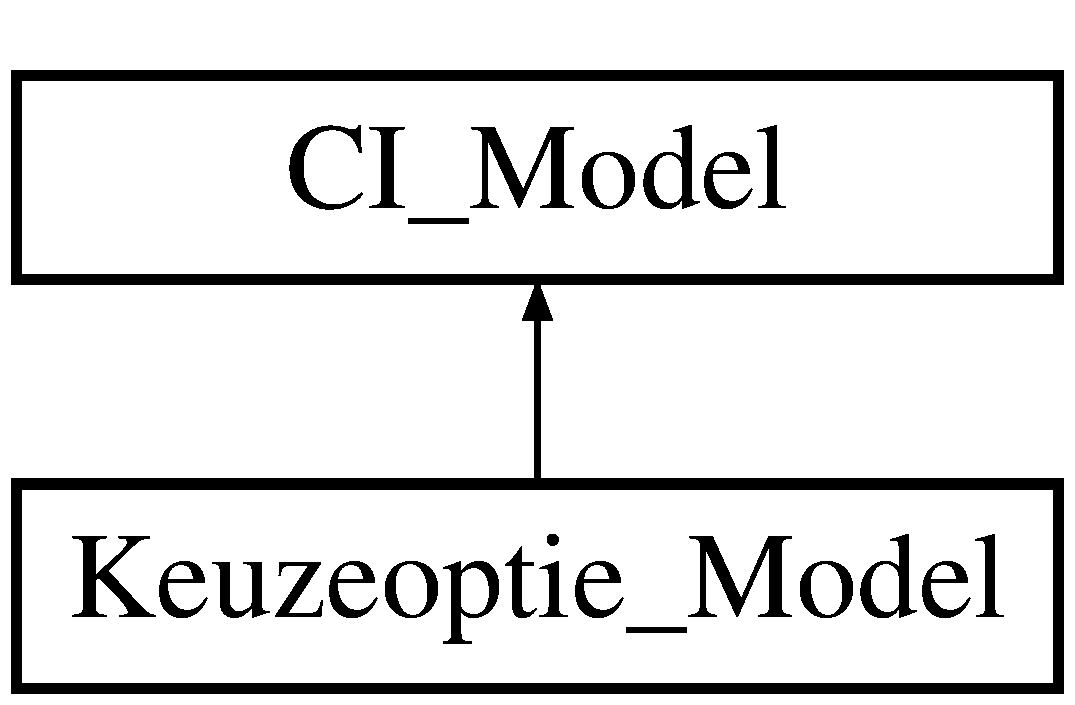
\includegraphics[height=2.000000cm]{class_keuzeoptie___model}
\end{center}
\end{figure}
\subsection*{Public Member Functions}
\begin{DoxyCompactItemize}
\item 
\mbox{\Hypertarget{class_keuzeoptie___model_a98d28a4d9a29d40c5a8aa0176f19a919}\label{class_keuzeoptie___model_a98d28a4d9a29d40c5a8aa0176f19a919}} 
{\bfseries get\+\_\+by\+Id} (\$id)
\item 
\mbox{\Hypertarget{class_keuzeoptie___model_a2b035b1ffd1cbe651b35bb3e53d72c09}\label{class_keuzeoptie___model_a2b035b1ffd1cbe651b35bb3e53d72c09}} 
{\bfseries get\+All\+By\+Naam} ()
\item 
\mbox{\Hypertarget{class_keuzeoptie___model_a6f3e4d26ab480501524eabb01683f5f7}\label{class_keuzeoptie___model_a6f3e4d26ab480501524eabb01683f5f7}} 
{\bfseries get\+All\+By\+Naam\+Where\+Keuze\+Mogelijkheid} (\$id)
\item 
\mbox{\Hypertarget{class_keuzeoptie___model_a9d98d1a6c3919a0e7b946d37fa385948}\label{class_keuzeoptie___model_a9d98d1a6c3919a0e7b946d37fa385948}} 
{\bfseries update} (\$keuzeoptie)
\item 
\mbox{\Hypertarget{class_keuzeoptie___model_a2452f524e794bc3f418d60cb296e19b5}\label{class_keuzeoptie___model_a2452f524e794bc3f418d60cb296e19b5}} 
{\bfseries add} (\$keuzeoptie)
\item 
\mbox{\Hypertarget{class_keuzeoptie___model_a2f8258add505482d7f00ea26493a5723}\label{class_keuzeoptie___model_a2f8258add505482d7f00ea26493a5723}} 
{\bfseries delete} (\$id)
\end{DoxyCompactItemize}


The documentation for this class was generated from the following file\+:\begin{DoxyCompactItemize}
\item 
application/models/Keuzeoptie\+\_\+model.\+php\end{DoxyCompactItemize}

\hypertarget{class_keuze_optie_van_deelnemer}{}\section{Keuze\+Optie\+Van\+Deelnemer Class Reference}
\label{class_keuze_optie_van_deelnemer}\index{Keuze\+Optie\+Van\+Deelnemer@{Keuze\+Optie\+Van\+Deelnemer}}


Controller voor functionaliteiten van keuzeoptie voor deelnemer.  


Inheritance diagram for Keuze\+Optie\+Van\+Deelnemer\+:\begin{figure}[H]
\begin{center}
\leavevmode
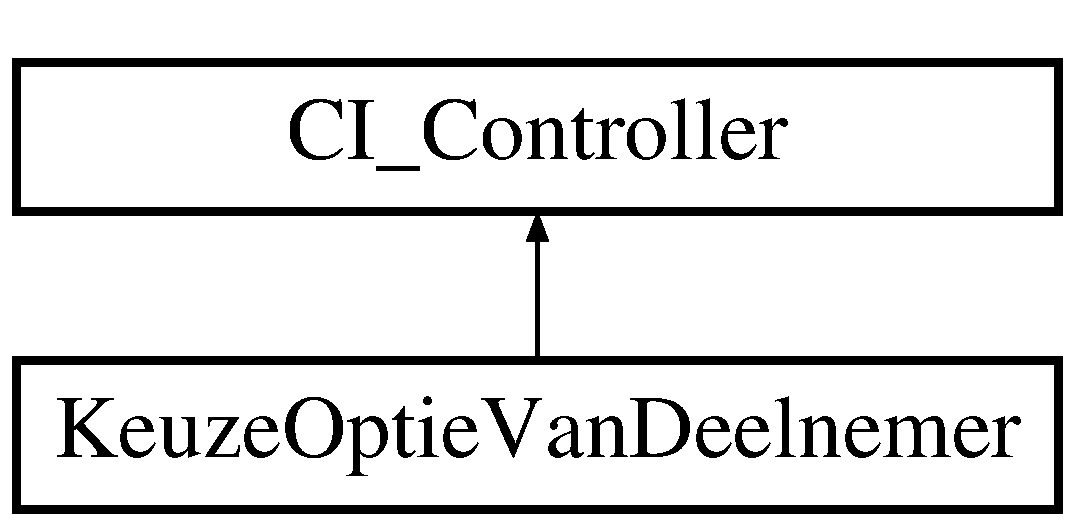
\includegraphics[height=2.000000cm]{class_keuze_optie_van_deelnemer}
\end{center}
\end{figure}
\subsection*{Public Member Functions}
\begin{DoxyCompactItemize}
\item 
\mbox{\hyperlink{class_keuze_optie_van_deelnemer_a04438616b87ca22ac662c94abc043c39}{update}} ()
\item 
\mbox{\Hypertarget{class_keuze_optie_van_deelnemer_af1516ec8cae4ca12ef73a5396c6df8e2}\label{class_keuze_optie_van_deelnemer_af1516ec8cae4ca12ef73a5396c6df8e2}} 
\mbox{\hyperlink{class_keuze_optie_van_deelnemer_af1516ec8cae4ca12ef73a5396c6df8e2}{deelnemer\+Aan\+Keuzeoptie\+Toevoegen}} (\$keuzeoptie\+Id, \$persoon\+Id)
\begin{DoxyCompactList}\small\item\em De keuzeoptie van de deelnemer wordt in de database opgeslagen. \end{DoxyCompactList}\item 
\mbox{\Hypertarget{class_keuze_optie_van_deelnemer_a9990c49ae295c91d1fa125b0d71d05d5}\label{class_keuze_optie_van_deelnemer_a9990c49ae295c91d1fa125b0d71d05d5}} 
\mbox{\hyperlink{class_keuze_optie_van_deelnemer_a9990c49ae295c91d1fa125b0d71d05d5}{deelnemer\+Van\+Keuzeoptie\+Verwijderen}} (\$keuzeoptie\+Id, \$persoon\+Id)
\begin{DoxyCompactList}\small\item\em De keuzeoptie van de deelnemer wordt weer uit de database verwijderd. \end{DoxyCompactList}\end{DoxyCompactItemize}


\subsection{Detailed Description}
Controller voor functionaliteiten van keuzeoptie voor deelnemer. 

\subsection{Member Function Documentation}
\mbox{\Hypertarget{class_keuze_optie_van_deelnemer_a04438616b87ca22ac662c94abc043c39}\label{class_keuze_optie_van_deelnemer_a04438616b87ca22ac662c94abc043c39}} 
\index{Keuze\+Optie\+Van\+Deelnemer@{Keuze\+Optie\+Van\+Deelnemer}!update@{update}}
\index{update@{update}!Keuze\+Optie\+Van\+Deelnemer@{Keuze\+Optie\+Van\+Deelnemer}}
\subsubsection{\texorpdfstring{update()}{update()}}
{\footnotesize\ttfamily Keuze\+Optie\+Van\+Deelnemer\+::update (\begin{DoxyParamCaption}{ }\end{DoxyParamCaption})}

klasse \mbox{\hyperlink{class_keuzeoptie}{Keuzeoptie}} aanmaken en initialiseren

Model inladen

\mbox{\hyperlink{class_keuzeoptie}{Keuzeoptie}} toevoegen of aanpassen

Redirect naar keuzemogelijkheid pagina 

The documentation for this class was generated from the following file\+:\begin{DoxyCompactItemize}
\item 
E\+:/\+D\+R\+I\+V\+E/\+C\+O\+L\+L\+E\+G\+E/\+T\+M/\+P0202/\+K\+P0201/\+R\+E\+P\+O/application/controllers/Keuzeoptie\+Van\+Deelnemer.\+php\end{DoxyCompactItemize}

\hypertarget{class_keuzeoptie_van_deelnemer___model}{}\section{Keuzeoptie\+Van\+Deelnemer\+\_\+\+Model Class Reference}
\label{class_keuzeoptie_van_deelnemer___model}\index{Keuzeoptie\+Van\+Deelnemer\+\_\+\+Model@{Keuzeoptie\+Van\+Deelnemer\+\_\+\+Model}}
Inheritance diagram for Keuzeoptie\+Van\+Deelnemer\+\_\+\+Model\+:\begin{figure}[H]
\begin{center}
\leavevmode
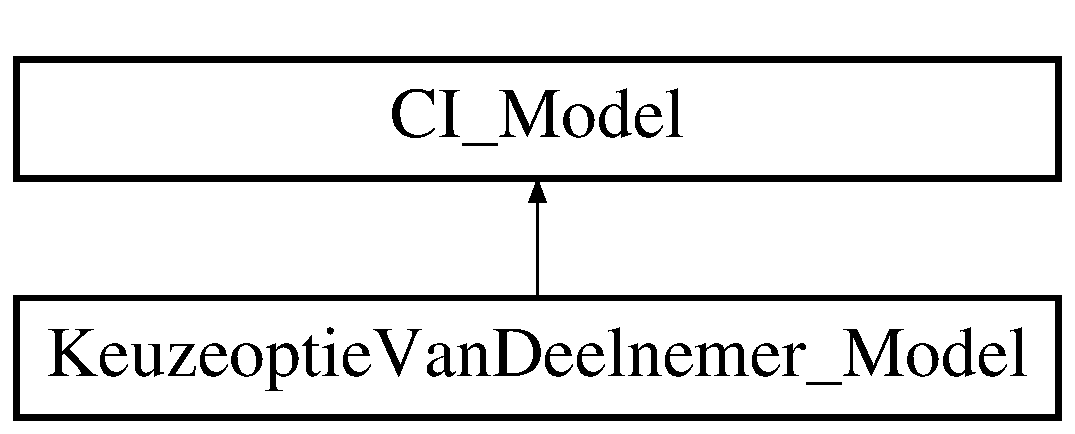
\includegraphics[height=2.000000cm]{class_keuzeoptie_van_deelnemer___model}
\end{center}
\end{figure}
\subsection*{Public Member Functions}
\begin{DoxyCompactItemize}
\item 
\mbox{\hyperlink{class_keuzeoptie_van_deelnemer___model_a095c5d389db211932136b53f25f39685}{\+\_\+\+\_\+construct}} ()
\item 
\mbox{\hyperlink{class_keuzeoptie_van_deelnemer___model_a5240031a73a1db935718f12ab29d80ad}{get\+\_\+by\+Keuzeoptie\+Id}} (\$id)
\begin{DoxyCompactList}\small\item\em opvragen van keuzeoptie door id mee te geven \end{DoxyCompactList}\item 
\mbox{\hyperlink{class_keuzeoptie_van_deelnemer___model_aa04bd86e024fed6b73b051c9cbb9ec52}{get\+\_\+by\+Persoon\+Id}} (\$id)
\begin{DoxyCompactList}\small\item\em opvragen van persoon door id mee te geven \end{DoxyCompactList}\item 
\mbox{\hyperlink{class_keuzeoptie_van_deelnemer___model_a59e9964aa59737ee3789f9458fdc4ee2}{add}} (\$Keuzeoptie\+Van\+Deelnemer)
\begin{DoxyCompactList}\small\item\em toevoegen van nieuwe keuzeoptie van een persoon aan de database \end{DoxyCompactList}\item 
\mbox{\hyperlink{class_keuzeoptie_van_deelnemer___model_af718b06f52e41eecd48c19b480fd237a}{delete}} (\$keuzeoptie\+Id, \$persoon\+Id)
\begin{DoxyCompactList}\small\item\em Verwijderen van keuzeoptie van een persoon uit de database. \end{DoxyCompactList}\end{DoxyCompactItemize}


\subsection{Constructor \& Destructor Documentation}
\mbox{\Hypertarget{class_keuzeoptie_van_deelnemer___model_a095c5d389db211932136b53f25f39685}\label{class_keuzeoptie_van_deelnemer___model_a095c5d389db211932136b53f25f39685}} 
\index{Keuzeoptie\+Van\+Deelnemer\+\_\+\+Model@{Keuzeoptie\+Van\+Deelnemer\+\_\+\+Model}!\+\_\+\+\_\+construct@{\+\_\+\+\_\+construct}}
\index{\+\_\+\+\_\+construct@{\+\_\+\+\_\+construct}!Keuzeoptie\+Van\+Deelnemer\+\_\+\+Model@{Keuzeoptie\+Van\+Deelnemer\+\_\+\+Model}}
\subsubsection{\texorpdfstring{\+\_\+\+\_\+construct()}{\_\_construct()}}
{\footnotesize\ttfamily \+\_\+\+\_\+construct (\begin{DoxyParamCaption}{ }\end{DoxyParamCaption})}



\subsection{Member Function Documentation}
\mbox{\Hypertarget{class_keuzeoptie_van_deelnemer___model_a59e9964aa59737ee3789f9458fdc4ee2}\label{class_keuzeoptie_van_deelnemer___model_a59e9964aa59737ee3789f9458fdc4ee2}} 
\index{Keuzeoptie\+Van\+Deelnemer\+\_\+\+Model@{Keuzeoptie\+Van\+Deelnemer\+\_\+\+Model}!add@{add}}
\index{add@{add}!Keuzeoptie\+Van\+Deelnemer\+\_\+\+Model@{Keuzeoptie\+Van\+Deelnemer\+\_\+\+Model}}
\subsubsection{\texorpdfstring{add()}{add()}}
{\footnotesize\ttfamily add (\begin{DoxyParamCaption}\item[{}]{\$\+Keuzeoptie\+Van\+Deelnemer }\end{DoxyParamCaption})}



toevoegen van nieuwe keuzeoptie van een persoon aan de database 

\mbox{\Hypertarget{class_keuzeoptie_van_deelnemer___model_af718b06f52e41eecd48c19b480fd237a}\label{class_keuzeoptie_van_deelnemer___model_af718b06f52e41eecd48c19b480fd237a}} 
\index{Keuzeoptie\+Van\+Deelnemer\+\_\+\+Model@{Keuzeoptie\+Van\+Deelnemer\+\_\+\+Model}!delete@{delete}}
\index{delete@{delete}!Keuzeoptie\+Van\+Deelnemer\+\_\+\+Model@{Keuzeoptie\+Van\+Deelnemer\+\_\+\+Model}}
\subsubsection{\texorpdfstring{delete()}{delete()}}
{\footnotesize\ttfamily delete (\begin{DoxyParamCaption}\item[{}]{\$keuzeoptie\+Id,  }\item[{}]{\$persoon\+Id }\end{DoxyParamCaption})}



Verwijderen van keuzeoptie van een persoon uit de database. 

\mbox{\Hypertarget{class_keuzeoptie_van_deelnemer___model_a5240031a73a1db935718f12ab29d80ad}\label{class_keuzeoptie_van_deelnemer___model_a5240031a73a1db935718f12ab29d80ad}} 
\index{Keuzeoptie\+Van\+Deelnemer\+\_\+\+Model@{Keuzeoptie\+Van\+Deelnemer\+\_\+\+Model}!get\+\_\+by\+Keuzeoptie\+Id@{get\+\_\+by\+Keuzeoptie\+Id}}
\index{get\+\_\+by\+Keuzeoptie\+Id@{get\+\_\+by\+Keuzeoptie\+Id}!Keuzeoptie\+Van\+Deelnemer\+\_\+\+Model@{Keuzeoptie\+Van\+Deelnemer\+\_\+\+Model}}
\subsubsection{\texorpdfstring{get\+\_\+by\+Keuzeoptie\+Id()}{get\_byKeuzeoptieId()}}
{\footnotesize\ttfamily get\+\_\+by\+Keuzeoptie\+Id (\begin{DoxyParamCaption}\item[{}]{\$id }\end{DoxyParamCaption})}



opvragen van keuzeoptie door id mee te geven 

\mbox{\Hypertarget{class_keuzeoptie_van_deelnemer___model_aa04bd86e024fed6b73b051c9cbb9ec52}\label{class_keuzeoptie_van_deelnemer___model_aa04bd86e024fed6b73b051c9cbb9ec52}} 
\index{Keuzeoptie\+Van\+Deelnemer\+\_\+\+Model@{Keuzeoptie\+Van\+Deelnemer\+\_\+\+Model}!get\+\_\+by\+Persoon\+Id@{get\+\_\+by\+Persoon\+Id}}
\index{get\+\_\+by\+Persoon\+Id@{get\+\_\+by\+Persoon\+Id}!Keuzeoptie\+Van\+Deelnemer\+\_\+\+Model@{Keuzeoptie\+Van\+Deelnemer\+\_\+\+Model}}
\subsubsection{\texorpdfstring{get\+\_\+by\+Persoon\+Id()}{get\_byPersoonId()}}
{\footnotesize\ttfamily get\+\_\+by\+Persoon\+Id (\begin{DoxyParamCaption}\item[{}]{\$id }\end{DoxyParamCaption})}



opvragen van persoon door id mee te geven 



The documentation for this class was generated from the following file\+:\begin{DoxyCompactItemize}
\item 
application/models/\mbox{\hyperlink{_keuzeoptie_van_deelnemer__model_8php}{Keuzeoptie\+Van\+Deelnemer\+\_\+model.\+php}}\end{DoxyCompactItemize}

\hypertarget{class_mail}{}\section{Mail Class Reference}
\label{class_mail}\index{Mail@{Mail}}


Controller voor mailfunctionaliteiten.  


Inheritance diagram for Mail\+:\begin{figure}[H]
\begin{center}
\leavevmode
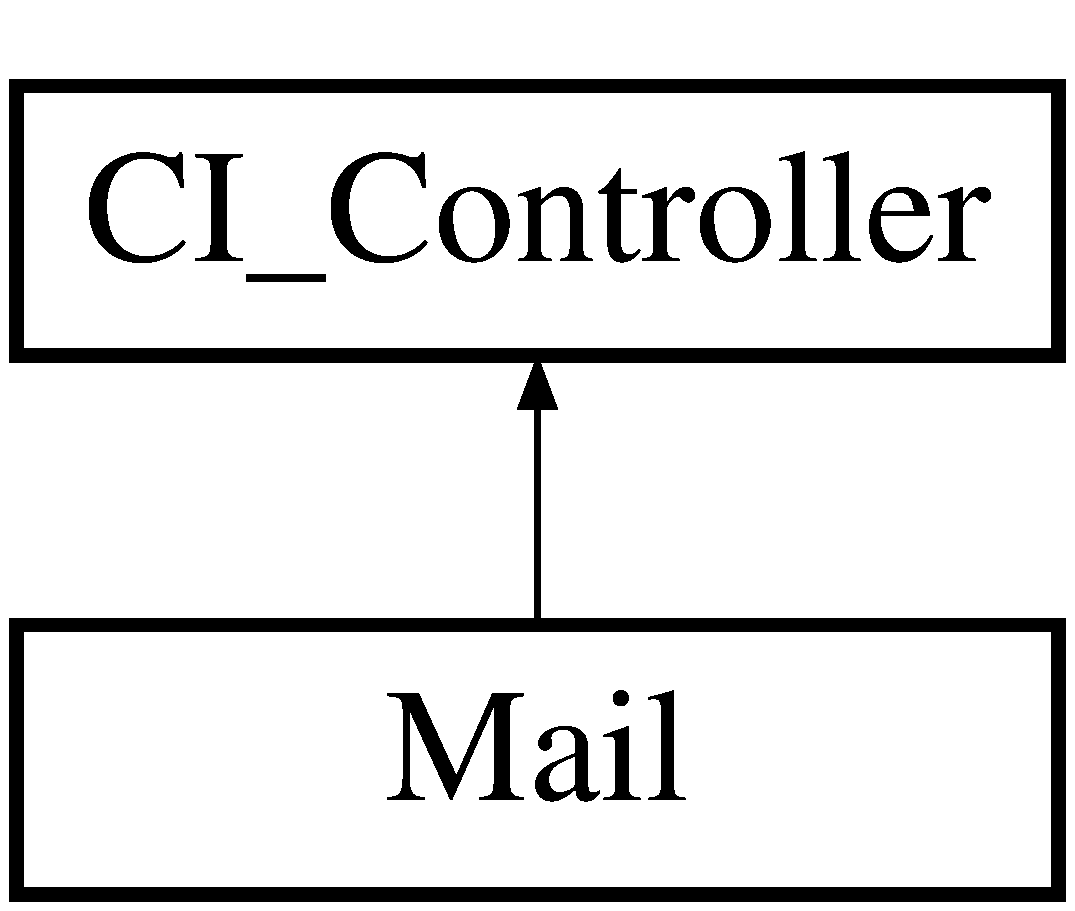
\includegraphics[height=2.000000cm]{class_mail}
\end{center}
\end{figure}
\subsection*{Public Member Functions}
\begin{DoxyCompactItemize}
\item 
\mbox{\Hypertarget{class_mail_a9e19643f7bd6b63ac867a99a42513790}\label{class_mail_a9e19643f7bd6b63ac867a99a42513790}} 
{\bfseries maakbericht} ()
\item 
\mbox{\Hypertarget{class_mail_a698adc5d93072946dbb03cb5e8025a92}\label{class_mail_a698adc5d93072946dbb03cb5e8025a92}} 
{\bfseries verstuur} ()
\item 
\mbox{\hyperlink{class_mail_a6b0bf7c864a3999c5b56222deb88874f}{remindervandaag}} ()
\item 
\mbox{\hyperlink{class_mail_a51675a2d0d65414634e3a21067462014}{maak\+Herinnering}} ()
\item 
\mbox{\hyperlink{class_mail_a5870a82a870b3b579d503101494abaf9}{verwijder\+Herinnering}} ()
\item 
\mbox{\hyperlink{class_mail_abb72118b34523cae188c03dc72955d8c}{overzicht}} ()
\item 
\mbox{\hyperlink{class_mail_a981094d50056d958426564d48c95cce1}{get\+\_\+\+Niet\+Ingeschreven}} ()
\item 
\mbox{\hyperlink{class_mail_af56bb11351090ce865a284a2c27ef3bb}{get\+Personen\+In\+Herinnering}} (\$id)
\end{DoxyCompactItemize}


\subsection{Detailed Description}
Controller voor mailfunctionaliteiten. 

\subsection{Member Function Documentation}
\mbox{\Hypertarget{class_mail_a981094d50056d958426564d48c95cce1}\label{class_mail_a981094d50056d958426564d48c95cce1}} 
\index{Mail@{Mail}!get\+\_\+\+Niet\+Ingeschreven@{get\+\_\+\+Niet\+Ingeschreven}}
\index{get\+\_\+\+Niet\+Ingeschreven@{get\+\_\+\+Niet\+Ingeschreven}!Mail@{Mail}}
\subsubsection{\texorpdfstring{get\+\_\+\+Niet\+Ingeschreven()}{get\_NietIngeschreven()}}
{\footnotesize\ttfamily Mail\+::get\+\_\+\+Niet\+Ingeschreven (\begin{DoxyParamCaption}{ }\end{DoxyParamCaption})}

Haalt niet ingeschreven personen op \mbox{\Hypertarget{class_mail_af56bb11351090ce865a284a2c27ef3bb}\label{class_mail_af56bb11351090ce865a284a2c27ef3bb}} 
\index{Mail@{Mail}!get\+Personen\+In\+Herinnering@{get\+Personen\+In\+Herinnering}}
\index{get\+Personen\+In\+Herinnering@{get\+Personen\+In\+Herinnering}!Mail@{Mail}}
\subsubsection{\texorpdfstring{get\+Personen\+In\+Herinnering()}{getPersonenInHerinnering()}}
{\footnotesize\ttfamily Mail\+::get\+Personen\+In\+Herinnering (\begin{DoxyParamCaption}\item[{}]{\$id }\end{DoxyParamCaption})}

s\+Haalt personen in herinnering op \$param int id Herinnering id \mbox{\Hypertarget{class_mail_a51675a2d0d65414634e3a21067462014}\label{class_mail_a51675a2d0d65414634e3a21067462014}} 
\index{Mail@{Mail}!maak\+Herinnering@{maak\+Herinnering}}
\index{maak\+Herinnering@{maak\+Herinnering}!Mail@{Mail}}
\subsubsection{\texorpdfstring{maak\+Herinnering()}{maakHerinnering()}}
{\footnotesize\ttfamily Mail\+::maak\+Herinnering (\begin{DoxyParamCaption}{ }\end{DoxyParamCaption})}

Maak een herinnering aan \mbox{\Hypertarget{class_mail_abb72118b34523cae188c03dc72955d8c}\label{class_mail_abb72118b34523cae188c03dc72955d8c}} 
\index{Mail@{Mail}!overzicht@{overzicht}}
\index{overzicht@{overzicht}!Mail@{Mail}}
\subsubsection{\texorpdfstring{overzicht()}{overzicht()}}
{\footnotesize\ttfamily Mail\+::overzicht (\begin{DoxyParamCaption}{ }\end{DoxyParamCaption})}

Laadt het overzichtspagina van alle mailherinneringen, sjablonen en ontvangers. \mbox{\Hypertarget{class_mail_a6b0bf7c864a3999c5b56222deb88874f}\label{class_mail_a6b0bf7c864a3999c5b56222deb88874f}} 
\index{Mail@{Mail}!remindervandaag@{remindervandaag}}
\index{remindervandaag@{remindervandaag}!Mail@{Mail}}
\subsubsection{\texorpdfstring{remindervandaag()}{remindervandaag()}}
{\footnotesize\ttfamily Mail\+::remindervandaag (\begin{DoxyParamCaption}{ }\end{DoxyParamCaption})}

Controleert of er vandaag mails moeten verstuurd worden, verstuurt diegene die van toepassing zijn \mbox{\Hypertarget{class_mail_a5870a82a870b3b579d503101494abaf9}\label{class_mail_a5870a82a870b3b579d503101494abaf9}} 
\index{Mail@{Mail}!verwijder\+Herinnering@{verwijder\+Herinnering}}
\index{verwijder\+Herinnering@{verwijder\+Herinnering}!Mail@{Mail}}
\subsubsection{\texorpdfstring{verwijder\+Herinnering()}{verwijderHerinnering()}}
{\footnotesize\ttfamily Mail\+::verwijder\+Herinnering (\begin{DoxyParamCaption}{ }\end{DoxyParamCaption})}

Verwijdert de herinnering, adhv Id 

The documentation for this class was generated from the following file\+:\begin{DoxyCompactItemize}
\item 
application/controllers/Mail.\+php\end{DoxyCompactItemize}

\hypertarget{class_mailherinnering__model}{}\section{Mailherinnering\+\_\+model Class Reference}
\label{class_mailherinnering__model}\index{Mailherinnering\+\_\+model@{Mailherinnering\+\_\+model}}
Inheritance diagram for Mailherinnering\+\_\+model\+:\begin{figure}[H]
\begin{center}
\leavevmode
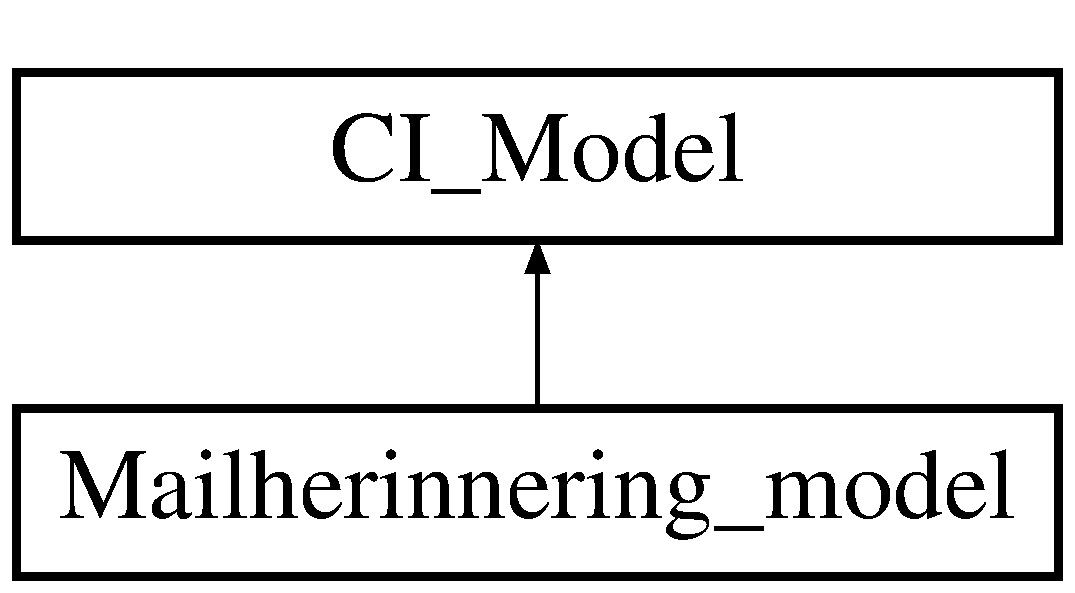
\includegraphics[height=2.000000cm]{class_mailherinnering__model}
\end{center}
\end{figure}
\subsection*{Public Member Functions}
\begin{DoxyCompactItemize}
\item 
\mbox{\hyperlink{class_mailherinnering__model_a29819479620b67d93965786bce00b695}{get\+\_\+\+Herinnering\+Dag}} (\$datum)
\item 
\mbox{\hyperlink{class_mailherinnering__model_aba0d5b303383fb5b1fabb5fd01cd3800}{get\+All}} ()
\item 
\mbox{\hyperlink{class_mailherinnering__model_a4c031458f8607c8960792706ce49f3ab}{get\+\_\+\+Personen\+In\+Reminder}} (\$reminder\+Id)
\item 
\mbox{\hyperlink{class_mailherinnering__model_a1ffebfb064147228f479c1d0b83ac50d}{insert}} (\$herinnering)
\item 
\mbox{\hyperlink{class_mailherinnering__model_a33e5747900292af47d92a2fd6ba4d484}{update}} (\$herinnering)
\item 
\mbox{\hyperlink{class_mailherinnering__model_aa4b59888d725b40a291f7e241fe60203}{delete}} (\$herinnering\+Id)
\end{DoxyCompactItemize}


\subsection{Member Function Documentation}
\mbox{\Hypertarget{class_mailherinnering__model_aa4b59888d725b40a291f7e241fe60203}\label{class_mailherinnering__model_aa4b59888d725b40a291f7e241fe60203}} 
\index{Mailherinnering\+\_\+model@{Mailherinnering\+\_\+model}!delete@{delete}}
\index{delete@{delete}!Mailherinnering\+\_\+model@{Mailherinnering\+\_\+model}}
\subsubsection{\texorpdfstring{delete()}{delete()}}
{\footnotesize\ttfamily delete (\begin{DoxyParamCaption}\item[{}]{\$herinnering\+Id }\end{DoxyParamCaption})}

\mbox{\Hypertarget{class_mailherinnering__model_a29819479620b67d93965786bce00b695}\label{class_mailherinnering__model_a29819479620b67d93965786bce00b695}} 
\index{Mailherinnering\+\_\+model@{Mailherinnering\+\_\+model}!get\+\_\+\+Herinnering\+Dag@{get\+\_\+\+Herinnering\+Dag}}
\index{get\+\_\+\+Herinnering\+Dag@{get\+\_\+\+Herinnering\+Dag}!Mailherinnering\+\_\+model@{Mailherinnering\+\_\+model}}
\subsubsection{\texorpdfstring{get\+\_\+\+Herinnering\+Dag()}{get\_HerinneringDag()}}
{\footnotesize\ttfamily get\+\_\+\+Herinnering\+Dag (\begin{DoxyParamCaption}\item[{}]{\$datum }\end{DoxyParamCaption})}

\mbox{\Hypertarget{class_mailherinnering__model_a4c031458f8607c8960792706ce49f3ab}\label{class_mailherinnering__model_a4c031458f8607c8960792706ce49f3ab}} 
\index{Mailherinnering\+\_\+model@{Mailherinnering\+\_\+model}!get\+\_\+\+Personen\+In\+Reminder@{get\+\_\+\+Personen\+In\+Reminder}}
\index{get\+\_\+\+Personen\+In\+Reminder@{get\+\_\+\+Personen\+In\+Reminder}!Mailherinnering\+\_\+model@{Mailherinnering\+\_\+model}}
\subsubsection{\texorpdfstring{get\+\_\+\+Personen\+In\+Reminder()}{get\_PersonenInReminder()}}
{\footnotesize\ttfamily get\+\_\+\+Personen\+In\+Reminder (\begin{DoxyParamCaption}\item[{}]{\$reminder\+Id }\end{DoxyParamCaption})}

\mbox{\Hypertarget{class_mailherinnering__model_aba0d5b303383fb5b1fabb5fd01cd3800}\label{class_mailherinnering__model_aba0d5b303383fb5b1fabb5fd01cd3800}} 
\index{Mailherinnering\+\_\+model@{Mailherinnering\+\_\+model}!get\+All@{get\+All}}
\index{get\+All@{get\+All}!Mailherinnering\+\_\+model@{Mailherinnering\+\_\+model}}
\subsubsection{\texorpdfstring{get\+All()}{getAll()}}
{\footnotesize\ttfamily get\+All (\begin{DoxyParamCaption}{ }\end{DoxyParamCaption})}

\mbox{\Hypertarget{class_mailherinnering__model_a1ffebfb064147228f479c1d0b83ac50d}\label{class_mailherinnering__model_a1ffebfb064147228f479c1d0b83ac50d}} 
\index{Mailherinnering\+\_\+model@{Mailherinnering\+\_\+model}!insert@{insert}}
\index{insert@{insert}!Mailherinnering\+\_\+model@{Mailherinnering\+\_\+model}}
\subsubsection{\texorpdfstring{insert()}{insert()}}
{\footnotesize\ttfamily insert (\begin{DoxyParamCaption}\item[{}]{\$herinnering }\end{DoxyParamCaption})}

\mbox{\Hypertarget{class_mailherinnering__model_a33e5747900292af47d92a2fd6ba4d484}\label{class_mailherinnering__model_a33e5747900292af47d92a2fd6ba4d484}} 
\index{Mailherinnering\+\_\+model@{Mailherinnering\+\_\+model}!update@{update}}
\index{update@{update}!Mailherinnering\+\_\+model@{Mailherinnering\+\_\+model}}
\subsubsection{\texorpdfstring{update()}{update()}}
{\footnotesize\ttfamily update (\begin{DoxyParamCaption}\item[{}]{\$herinnering }\end{DoxyParamCaption})}



The documentation for this class was generated from the following file\+:\begin{DoxyCompactItemize}
\item 
application/models/\mbox{\hyperlink{_mailherinnering__model_8php}{Mailherinnering\+\_\+model.\+php}}\end{DoxyCompactItemize}

\hypertarget{class_mailsjabloon__model}{}\section{Mailsjabloon\+\_\+model Class Reference}
\label{class_mailsjabloon__model}\index{Mailsjabloon\+\_\+model@{Mailsjabloon\+\_\+model}}
Inheritance diagram for Mailsjabloon\+\_\+model\+:\begin{figure}[H]
\begin{center}
\leavevmode
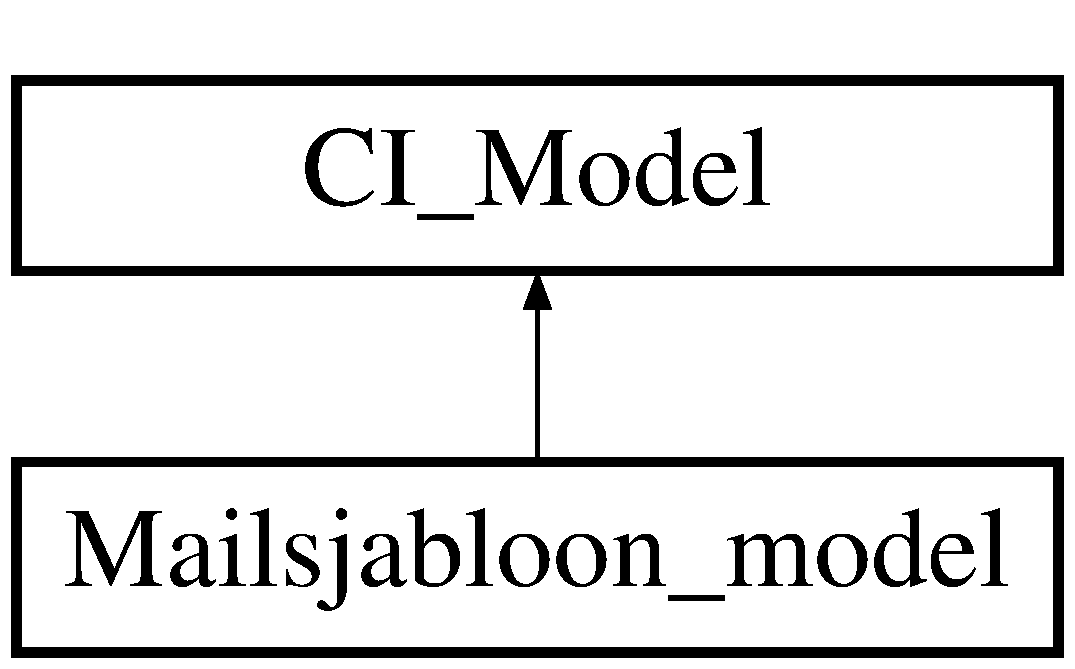
\includegraphics[height=2.000000cm]{class_mailsjabloon__model}
\end{center}
\end{figure}
\subsection*{Public Member Functions}
\begin{DoxyCompactItemize}
\item 
\mbox{\Hypertarget{class_mailsjabloon__model_a2fd2620c0951e3b9954e557652b74ff0}\label{class_mailsjabloon__model_a2fd2620c0951e3b9954e557652b74ff0}} 
{\bfseries get} (\$id)
\item 
\mbox{\Hypertarget{class_mailsjabloon__model_a6723ec4f9fa1a3f1195f93f0c9326239}\label{class_mailsjabloon__model_a6723ec4f9fa1a3f1195f93f0c9326239}} 
{\bfseries get\+All} ()
\item 
\mbox{\Hypertarget{class_mailsjabloon__model_a4272406d2eee5775d951d5320d0618aa}\label{class_mailsjabloon__model_a4272406d2eee5775d951d5320d0618aa}} 
{\bfseries update} (\$mailsjabloon)
\item 
\mbox{\Hypertarget{class_mailsjabloon__model_ac8906f2f6b9aedabd697ab35ce11e407}\label{class_mailsjabloon__model_ac8906f2f6b9aedabd697ab35ce11e407}} 
{\bfseries add} (\$mailsjabloon)
\end{DoxyCompactItemize}


The documentation for this class was generated from the following file\+:\begin{DoxyCompactItemize}
\item 
application/models/Mailsjabloon\+\_\+model.\+php\end{DoxyCompactItemize}

\hypertarget{class_main}{}\section{Main Class Reference}
\label{class_main}\index{Main@{Main}}
Inheritance diagram for Main\+:\begin{figure}[H]
\begin{center}
\leavevmode
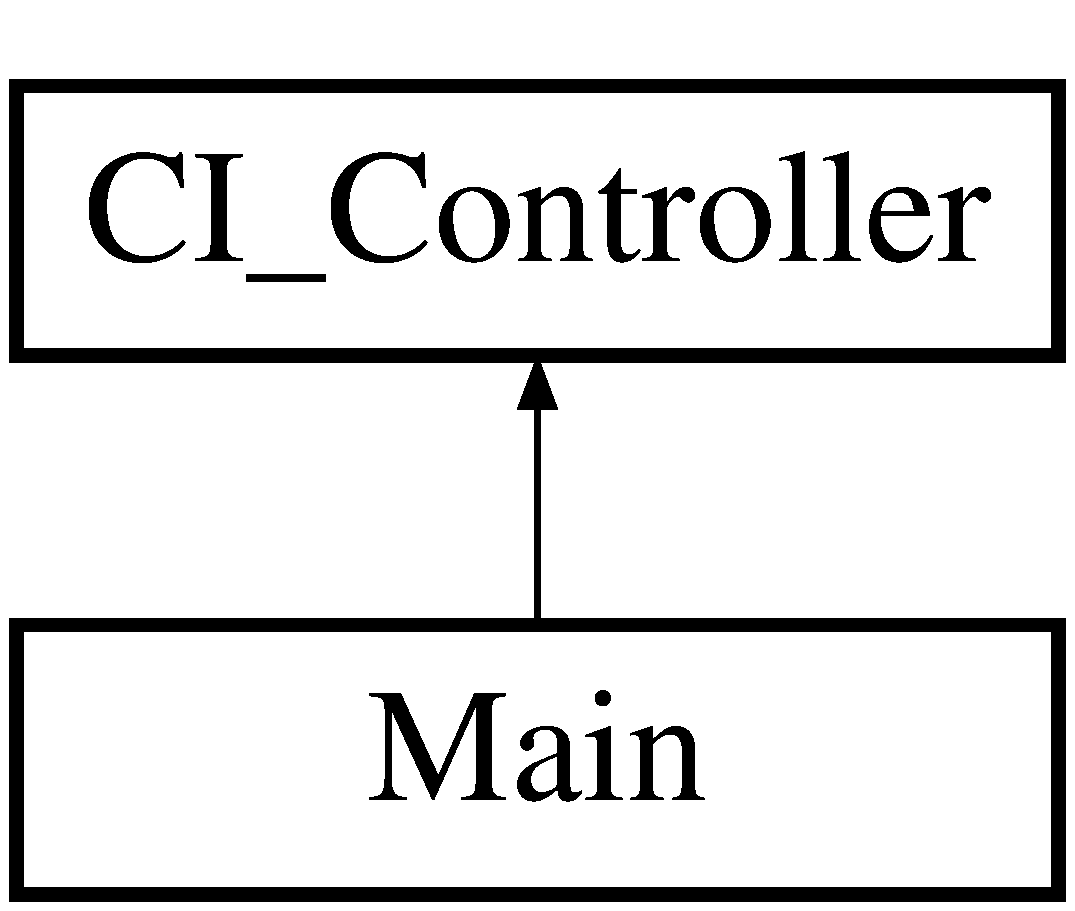
\includegraphics[height=2.000000cm]{class_main}
\end{center}
\end{figure}
\subsection*{Public Member Functions}
\begin{DoxyCompactItemize}
\item 
\mbox{\Hypertarget{class_main_a581fc1016bc76cba4fad0fc9a9f3f9cd}\label{class_main_a581fc1016bc76cba4fad0fc9a9f3f9cd}} 
{\bfseries signin} (\$id=null, \$token=null)
\end{DoxyCompactItemize}


The documentation for this class was generated from the following file\+:\begin{DoxyCompactItemize}
\item 
application/controllers/Main.\+php\end{DoxyCompactItemize}

\hypertarget{class_persoon__model}{}\section{Persoon\+\_\+model Class Reference}
\label{class_persoon__model}\index{Persoon\+\_\+model@{Persoon\+\_\+model}}
Inheritance diagram for Persoon\+\_\+model\+:\begin{figure}[H]
\begin{center}
\leavevmode
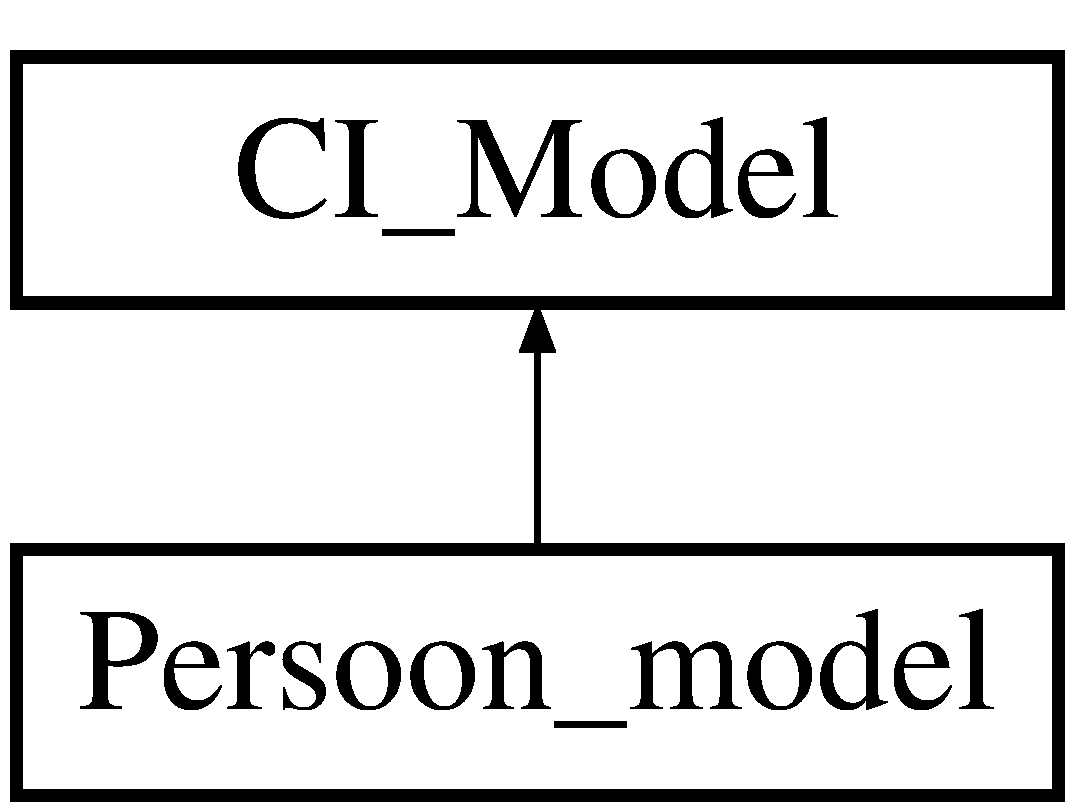
\includegraphics[height=2.000000cm]{class_persoon__model}
\end{center}
\end{figure}
\subsection*{Public Member Functions}
\begin{DoxyCompactItemize}
\item 
\mbox{\Hypertarget{class_persoon__model_a4fe7a2f8ac42cd4901ef68b06358d93f}\label{class_persoon__model_a4fe7a2f8ac42cd4901ef68b06358d93f}} 
{\bfseries get\+\_\+by\+Id\+And\+Token} (\$id, \$token)
\item 
\mbox{\Hypertarget{class_persoon__model_a98d28a4d9a29d40c5a8aa0176f19a919}\label{class_persoon__model_a98d28a4d9a29d40c5a8aa0176f19a919}} 
{\bfseries get\+\_\+by\+Id} (\$id)
\item 
\mbox{\Hypertarget{class_persoon__model_a8d14f8e8d18daadab52042074396a6b8}\label{class_persoon__model_a8d14f8e8d18daadab52042074396a6b8}} 
{\bfseries get\+\_\+\+Id} (\$id)
\item 
\mbox{\Hypertarget{class_persoon__model_a7e94dd1f7edfacea0d0814ff027b7e04}\label{class_persoon__model_a7e94dd1f7edfacea0d0814ff027b7e04}} 
{\bfseries get\+\_\+\+All} ()
\item 
\mbox{\Hypertarget{class_persoon__model_a7e0633aa62a76b8fb9bf35c6167a2a0f}\label{class_persoon__model_a7e0633aa62a76b8fb9bf35c6167a2a0f}} 
{\bfseries get\+\_\+\+All\+Deelnemers} ()
\item 
\mbox{\Hypertarget{class_persoon__model_a34374012facb64562423057666ed535d}\label{class_persoon__model_a34374012facb64562423057666ed535d}} 
{\bfseries get\+\_\+\+All\+Vrijwilligers} ()
\item 
\mbox{\Hypertarget{class_persoon__model_ae20838d9cd61c63ac26fdb07f4b7bff4}\label{class_persoon__model_ae20838d9cd61c63ac26fdb07f4b7bff4}} 
{\bfseries get\+\_\+\+Niet\+Ingeschreven\+Vrijwilligers} ()
\item 
\mbox{\Hypertarget{class_persoon__model_a6a34ff3e55e35289c802e4e4ac14792d}\label{class_persoon__model_a6a34ff3e55e35289c802e4e4ac14792d}} 
{\bfseries get\+\_\+\+Niet\+Ingeschreven\+Deelnemers} ()
\item 
\mbox{\Hypertarget{class_persoon__model_abb16337bee193e227f25cb9e37ac9394}\label{class_persoon__model_abb16337bee193e227f25cb9e37ac9394}} 
{\bfseries insert} (\$persoon)
\item 
\mbox{\Hypertarget{class_persoon__model_a40ea86b0c55c207673f65d23a4a8e98d}\label{class_persoon__model_a40ea86b0c55c207673f65d23a4a8e98d}} 
{\bfseries generatetoken} ()
\item 
\mbox{\Hypertarget{class_persoon__model_aad1045b9fabfabcb3090fb0b0b17a6e6}\label{class_persoon__model_aad1045b9fabfabcb3090fb0b0b17a6e6}} 
{\bfseries get\+\_\+bytoken} (\$token)
\item 
\mbox{\Hypertarget{class_persoon__model_a20a10592218dbf11fd43c955ce5fcee1}\label{class_persoon__model_a20a10592218dbf11fd43c955ce5fcee1}} 
{\bfseries getallwithactiviteit} ()
\item 
\mbox{\Hypertarget{class_persoon__model_aba5a7a9b6a803620d0fddcbfffa83148}\label{class_persoon__model_aba5a7a9b6a803620d0fddcbfffa83148}} 
{\bfseries get\+All\+\_\+of\+Jaargang} (\$jaargang\+Id)
\item 
\mbox{\Hypertarget{class_persoon__model_afa062e8195502a034cfa2780c6763cf6}\label{class_persoon__model_afa062e8195502a034cfa2780c6763cf6}} 
{\bfseries get\+All\+\_\+of\+Jaargang\+\_\+with\+Shift} (\$jaargang\+Id)
\item 
\mbox{\Hypertarget{class_persoon__model_a9169319ec748964dc67f0f640d182250}\label{class_persoon__model_a9169319ec748964dc67f0f640d182250}} 
{\bfseries get\+All} (\$id)
\end{DoxyCompactItemize}


The documentation for this class was generated from the following file\+:\begin{DoxyCompactItemize}
\item 
application/models/Persoon\+\_\+model.\+php\end{DoxyCompactItemize}

\hypertarget{class_persoon_in_herinnering__model}{}\section{Persoon\+In\+Herinnering\+\_\+model Class Reference}
\label{class_persoon_in_herinnering__model}\index{Persoon\+In\+Herinnering\+\_\+model@{Persoon\+In\+Herinnering\+\_\+model}}
Inheritance diagram for Persoon\+In\+Herinnering\+\_\+model\+:\begin{figure}[H]
\begin{center}
\leavevmode
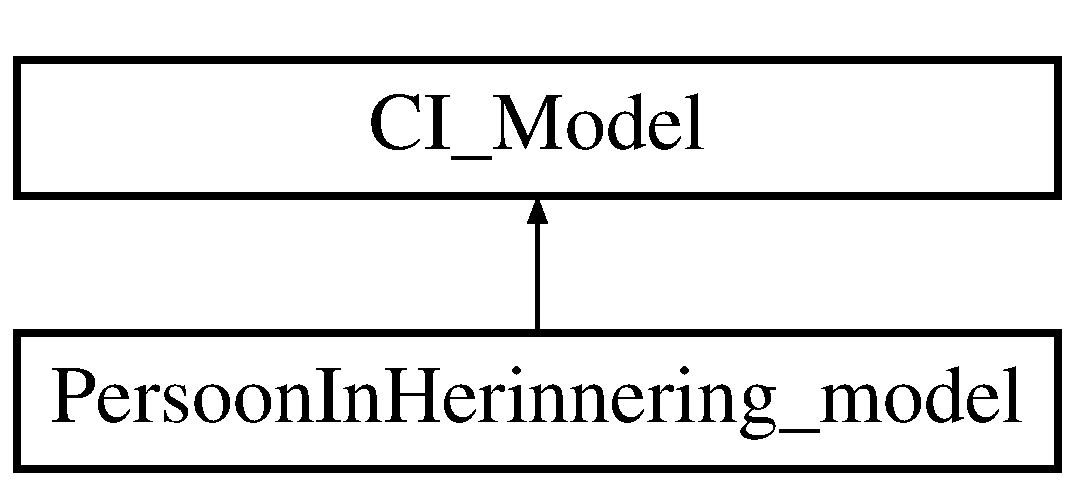
\includegraphics[height=2.000000cm]{class_persoon_in_herinnering__model}
\end{center}
\end{figure}
\subsection*{Public Member Functions}
\begin{DoxyCompactItemize}
\item 
\mbox{\hyperlink{class_persoon_in_herinnering__model_a9dd863caf95bb6dda565526e3892c2b5}{\+\_\+\+\_\+construct}} ()
\item 
\mbox{\hyperlink{class_persoon_in_herinnering__model_aae7c684767759ee244cf1e190a516952}{get\+\_\+by\+Herinnering\+Id}} (\$id)
\item 
\mbox{\hyperlink{class_persoon_in_herinnering__model_ab19b43169595548f27dd52a93a81ab9b}{insert}} (\$persoon\+Inherinnering)
\item 
\mbox{\hyperlink{class_persoon_in_herinnering__model_acdf0cb89162001b81f64a36eb8bd7663}{delete}} (\$herinnering\+Id)
\end{DoxyCompactItemize}


\subsection{Constructor \& Destructor Documentation}
\mbox{\Hypertarget{class_persoon_in_herinnering__model_a9dd863caf95bb6dda565526e3892c2b5}\label{class_persoon_in_herinnering__model_a9dd863caf95bb6dda565526e3892c2b5}} 
\index{Persoon\+In\+Herinnering\+\_\+model@{Persoon\+In\+Herinnering\+\_\+model}!\+\_\+\+\_\+construct@{\+\_\+\+\_\+construct}}
\index{\+\_\+\+\_\+construct@{\+\_\+\+\_\+construct}!Persoon\+In\+Herinnering\+\_\+model@{Persoon\+In\+Herinnering\+\_\+model}}
\subsubsection{\texorpdfstring{\+\_\+\+\_\+construct()}{\_\_construct()}}
{\footnotesize\ttfamily Persoon\+In\+Herinnering\+\_\+model\+::\+\_\+\+\_\+construct (\begin{DoxyParamCaption}{ }\end{DoxyParamCaption})}

Default constructor 

\subsection{Member Function Documentation}
\mbox{\Hypertarget{class_persoon_in_herinnering__model_acdf0cb89162001b81f64a36eb8bd7663}\label{class_persoon_in_herinnering__model_acdf0cb89162001b81f64a36eb8bd7663}} 
\index{Persoon\+In\+Herinnering\+\_\+model@{Persoon\+In\+Herinnering\+\_\+model}!delete@{delete}}
\index{delete@{delete}!Persoon\+In\+Herinnering\+\_\+model@{Persoon\+In\+Herinnering\+\_\+model}}
\subsubsection{\texorpdfstring{delete()}{delete()}}
{\footnotesize\ttfamily Persoon\+In\+Herinnering\+\_\+model\+::delete (\begin{DoxyParamCaption}\item[{}]{\$herinnering\+Id }\end{DoxyParamCaption})}

Verwijderd de persoon in een specifieke herinnering 
\begin{DoxyParams}[1]{Parameters}
int & {\em \$id} & Id van Herinnering \\
\hline
\end{DoxyParams}
\mbox{\Hypertarget{class_persoon_in_herinnering__model_aae7c684767759ee244cf1e190a516952}\label{class_persoon_in_herinnering__model_aae7c684767759ee244cf1e190a516952}} 
\index{Persoon\+In\+Herinnering\+\_\+model@{Persoon\+In\+Herinnering\+\_\+model}!get\+\_\+by\+Herinnering\+Id@{get\+\_\+by\+Herinnering\+Id}}
\index{get\+\_\+by\+Herinnering\+Id@{get\+\_\+by\+Herinnering\+Id}!Persoon\+In\+Herinnering\+\_\+model@{Persoon\+In\+Herinnering\+\_\+model}}
\subsubsection{\texorpdfstring{get\+\_\+by\+Herinnering\+Id()}{get\_byHerinneringId()}}
{\footnotesize\ttfamily Persoon\+In\+Herinnering\+\_\+model\+::get\+\_\+by\+Herinnering\+Id (\begin{DoxyParamCaption}\item[{}]{\$id }\end{DoxyParamCaption})}

Haalt een emailherinnering op 
\begin{DoxyParams}[1]{Parameters}
int & {\em \$id} & Id van emailherinnering \\
\hline
\end{DoxyParams}
\mbox{\Hypertarget{class_persoon_in_herinnering__model_ab19b43169595548f27dd52a93a81ab9b}\label{class_persoon_in_herinnering__model_ab19b43169595548f27dd52a93a81ab9b}} 
\index{Persoon\+In\+Herinnering\+\_\+model@{Persoon\+In\+Herinnering\+\_\+model}!insert@{insert}}
\index{insert@{insert}!Persoon\+In\+Herinnering\+\_\+model@{Persoon\+In\+Herinnering\+\_\+model}}
\subsubsection{\texorpdfstring{insert()}{insert()}}
{\footnotesize\ttfamily Persoon\+In\+Herinnering\+\_\+model\+::insert (\begin{DoxyParamCaption}\item[{}]{\$persoon\+Inherinnering }\end{DoxyParamCaption})}

Maakt een nieuwe record aan voor persoon in herinnering 
\begin{DoxyParams}[1]{Parameters}
int & {\em \$id} & Persoon\+In\+Herinnering object \\
\hline
\end{DoxyParams}


The documentation for this class was generated from the following file\+:\begin{DoxyCompactItemize}
\item 
application/models/Persoon\+In\+Herinnering\+\_\+model.\+php\end{DoxyCompactItemize}

\hypertarget{class_plaats}{}\section{Plaats Class Reference}
\label{class_plaats}\index{Plaats@{Plaats}}
Inheritance diagram for Plaats\+:\begin{figure}[H]
\begin{center}
\leavevmode
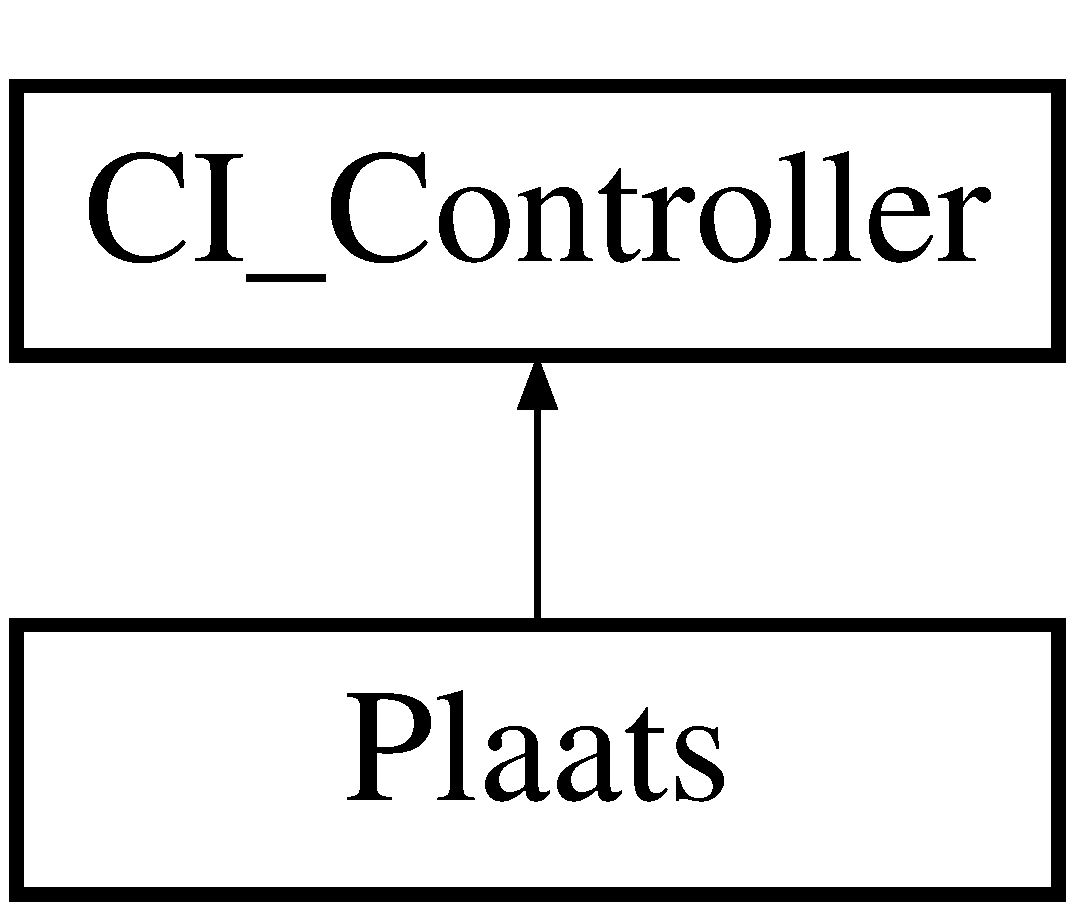
\includegraphics[height=2.000000cm]{class_plaats}
\end{center}
\end{figure}
\subsection*{Public Member Functions}
\begin{DoxyCompactItemize}
\item 
\mbox{\hyperlink{class_plaats_a095c5d389db211932136b53f25f39685}{\+\_\+\+\_\+construct}} ()
\item 
\mbox{\hyperlink{class_plaats_a3a5c8647f1efcdff577c49894a2bdde8}{get\+Empty\+Plaats}} ()
\begin{DoxyCompactList}\small\item\em Geeft nieuw leeg plaatsobject. \end{DoxyCompactList}\item 
\mbox{\hyperlink{class_plaats_a7e7e04e0718668180cf4e8fb0b4dea9b}{maak\+Nieuwe}} ()
\begin{DoxyCompactList}\small\item\em maak nieuw plaatsobject \end{DoxyCompactList}\item 
\mbox{\hyperlink{class_plaats_a6db5689af94fb09c1652e5f3b1d2770a}{registreer}} ()
\begin{DoxyCompactList}\small\item\em Registreer wat de administrator invult. Als hij op wijzig klikt, wordt het bestaande plaatsobject geupdatet. Wanneer hij een nieuwe plaats toevoegt (en dus gewoon de veldjes invult zonder op wijzig geklikt te hebben), wordt het nieuwe plaatsobject in de database geïnsert. \end{DoxyCompactList}\item 
\mbox{\hyperlink{class_plaats_aa5997c2d1474e374ea50a87e8673d2e4}{verwijder}} (\$id)
\begin{DoxyCompactList}\small\item\em Functie om een locatie uit de database te verwijderen. \end{DoxyCompactList}\item 
\mbox{\hyperlink{class_plaats_aa10f6589c4f171a54524ed6758bed97f}{wijzig}} (\$id)
\begin{DoxyCompactList}\small\item\em Functie om een bestaande locatie te wijzigen in de database. \end{DoxyCompactList}\item 
\mbox{\hyperlink{class_plaats_aeac29d4165c8a50a862fe3e8df220376}{jsonplaats}} (\$id)
\begin{DoxyCompactList}\small\item\em Functie om plaats op te halen. \end{DoxyCompactList}\end{DoxyCompactItemize}


\subsection{Constructor \& Destructor Documentation}
\mbox{\Hypertarget{class_plaats_a095c5d389db211932136b53f25f39685}\label{class_plaats_a095c5d389db211932136b53f25f39685}} 
\index{Plaats@{Plaats}!\+\_\+\+\_\+construct@{\+\_\+\+\_\+construct}}
\index{\+\_\+\+\_\+construct@{\+\_\+\+\_\+construct}!Plaats@{Plaats}}
\subsubsection{\texorpdfstring{\+\_\+\+\_\+construct()}{\_\_construct()}}
{\footnotesize\ttfamily \+\_\+\+\_\+construct (\begin{DoxyParamCaption}{ }\end{DoxyParamCaption})}



\subsection{Member Function Documentation}
\mbox{\Hypertarget{class_plaats_a3a5c8647f1efcdff577c49894a2bdde8}\label{class_plaats_a3a5c8647f1efcdff577c49894a2bdde8}} 
\index{Plaats@{Plaats}!get\+Empty\+Plaats@{get\+Empty\+Plaats}}
\index{get\+Empty\+Plaats@{get\+Empty\+Plaats}!Plaats@{Plaats}}
\subsubsection{\texorpdfstring{get\+Empty\+Plaats()}{getEmptyPlaats()}}
{\footnotesize\ttfamily get\+Empty\+Plaats (\begin{DoxyParamCaption}{ }\end{DoxyParamCaption})}



Geeft nieuw leeg plaatsobject. 

\mbox{\Hypertarget{class_plaats_aeac29d4165c8a50a862fe3e8df220376}\label{class_plaats_aeac29d4165c8a50a862fe3e8df220376}} 
\index{Plaats@{Plaats}!jsonplaats@{jsonplaats}}
\index{jsonplaats@{jsonplaats}!Plaats@{Plaats}}
\subsubsection{\texorpdfstring{jsonplaats()}{jsonplaats()}}
{\footnotesize\ttfamily jsonplaats (\begin{DoxyParamCaption}\item[{}]{\$id }\end{DoxyParamCaption})}



Functie om plaats op te halen. 

\mbox{\Hypertarget{class_plaats_a7e7e04e0718668180cf4e8fb0b4dea9b}\label{class_plaats_a7e7e04e0718668180cf4e8fb0b4dea9b}} 
\index{Plaats@{Plaats}!maak\+Nieuwe@{maak\+Nieuwe}}
\index{maak\+Nieuwe@{maak\+Nieuwe}!Plaats@{Plaats}}
\subsubsection{\texorpdfstring{maak\+Nieuwe()}{maakNieuwe()}}
{\footnotesize\ttfamily maak\+Nieuwe (\begin{DoxyParamCaption}{ }\end{DoxyParamCaption})}



maak nieuw plaatsobject 

\mbox{\Hypertarget{class_plaats_a6db5689af94fb09c1652e5f3b1d2770a}\label{class_plaats_a6db5689af94fb09c1652e5f3b1d2770a}} 
\index{Plaats@{Plaats}!registreer@{registreer}}
\index{registreer@{registreer}!Plaats@{Plaats}}
\subsubsection{\texorpdfstring{registreer()}{registreer()}}
{\footnotesize\ttfamily registreer (\begin{DoxyParamCaption}{ }\end{DoxyParamCaption})}



Registreer wat de administrator invult. Als hij op wijzig klikt, wordt het bestaande plaatsobject geupdatet. Wanneer hij een nieuwe plaats toevoegt (en dus gewoon de veldjes invult zonder op wijzig geklikt te hebben), wordt het nieuwe plaatsobject in de database geïnsert. 

\mbox{\Hypertarget{class_plaats_aa5997c2d1474e374ea50a87e8673d2e4}\label{class_plaats_aa5997c2d1474e374ea50a87e8673d2e4}} 
\index{Plaats@{Plaats}!verwijder@{verwijder}}
\index{verwijder@{verwijder}!Plaats@{Plaats}}
\subsubsection{\texorpdfstring{verwijder()}{verwijder()}}
{\footnotesize\ttfamily verwijder (\begin{DoxyParamCaption}\item[{}]{\$id }\end{DoxyParamCaption})}



Functie om een locatie uit de database te verwijderen. 

\mbox{\Hypertarget{class_plaats_aa10f6589c4f171a54524ed6758bed97f}\label{class_plaats_aa10f6589c4f171a54524ed6758bed97f}} 
\index{Plaats@{Plaats}!wijzig@{wijzig}}
\index{wijzig@{wijzig}!Plaats@{Plaats}}
\subsubsection{\texorpdfstring{wijzig()}{wijzig()}}
{\footnotesize\ttfamily wijzig (\begin{DoxyParamCaption}\item[{}]{\$id }\end{DoxyParamCaption})}



Functie om een bestaande locatie te wijzigen in de database. 



The documentation for this class was generated from the following file\+:\begin{DoxyCompactItemize}
\item 
application/controllers/\mbox{\hyperlink{_plaats_8php}{Plaats.\+php}}\end{DoxyCompactItemize}

\hypertarget{class_plaats__model}{}\section{Plaats\+\_\+model Class Reference}
\label{class_plaats__model}\index{Plaats\+\_\+model@{Plaats\+\_\+model}}
Inheritance diagram for Plaats\+\_\+model\+:\begin{figure}[H]
\begin{center}
\leavevmode
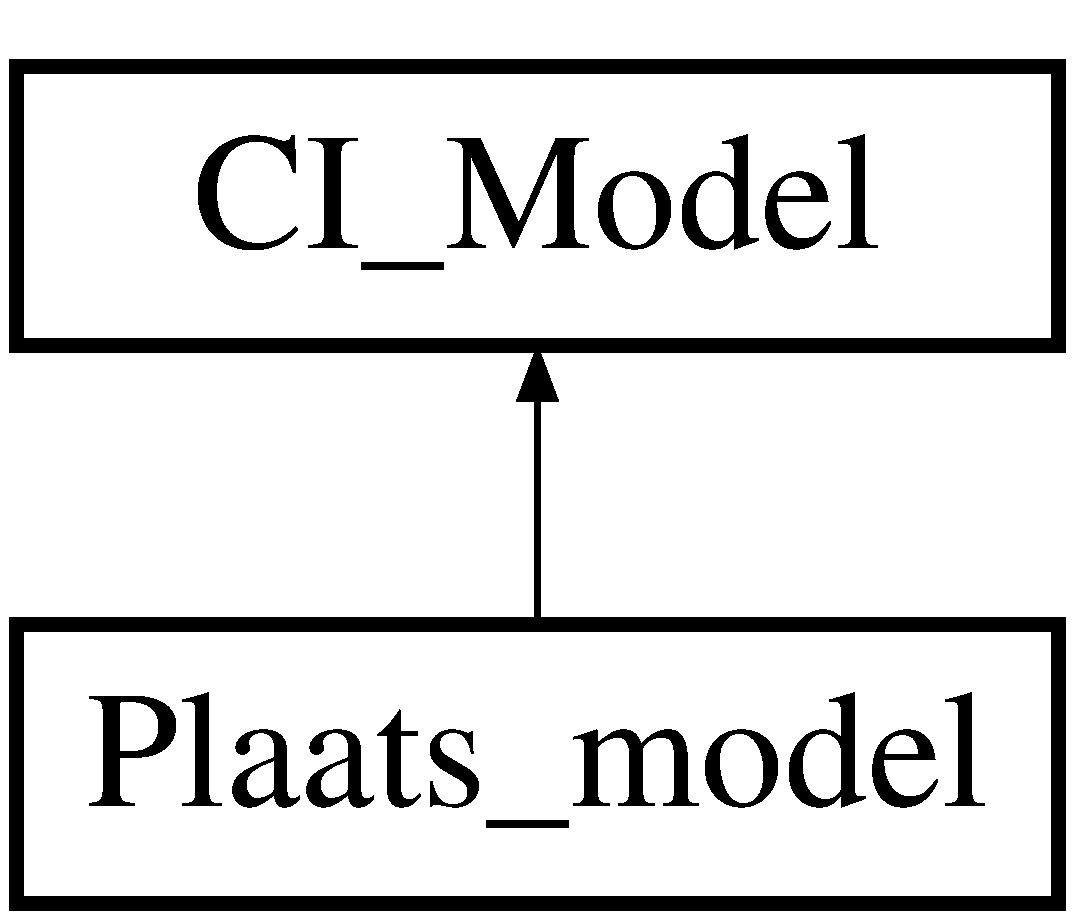
\includegraphics[height=2.000000cm]{class_plaats__model}
\end{center}
\end{figure}
\subsection*{Public Member Functions}
\begin{DoxyCompactItemize}
\item 
\mbox{\Hypertarget{class_plaats__model_a39dfb5046fda394e79bc2b17c0d8bd1f}\label{class_plaats__model_a39dfb5046fda394e79bc2b17c0d8bd1f}} 
\mbox{\hyperlink{class_plaats__model_a39dfb5046fda394e79bc2b17c0d8bd1f}{get\+All\+By\+Plaatsnaam}} ()
\begin{DoxyCompactList}\small\item\em functie om alle plaatsen uit de database op te vragen \end{DoxyCompactList}\item 
\mbox{\hyperlink{class_plaats__model_ad74fde1e8efdd97f181c649e8d869590}{get\+Plaats\+By\+Id}} (\$id)
\item 
\mbox{\hyperlink{class_plaats__model_a708c9f18b63ac2655c6121e63b5ffe7f}{insert}} (\$plaats)
\item 
\mbox{\hyperlink{class_plaats__model_ac03a8dd14ad6cf143baca5f054ab94a1}{update}} (\$plaats)
\item 
\mbox{\hyperlink{class_plaats__model_aed60da9232b9f683e0d9d62897e43cd7}{delete}} (\$id)
\end{DoxyCompactItemize}


\subsection{Member Function Documentation}
\mbox{\Hypertarget{class_plaats__model_aed60da9232b9f683e0d9d62897e43cd7}\label{class_plaats__model_aed60da9232b9f683e0d9d62897e43cd7}} 
\index{Plaats\+\_\+model@{Plaats\+\_\+model}!delete@{delete}}
\index{delete@{delete}!Plaats\+\_\+model@{Plaats\+\_\+model}}
\subsubsection{\texorpdfstring{delete()}{delete()}}
{\footnotesize\ttfamily Plaats\+\_\+model\+::delete (\begin{DoxyParamCaption}\item[{}]{\$id }\end{DoxyParamCaption})}

functie om plaats te verwijderen uit de database per id 
\begin{DoxyParams}[1]{Parameters}
string & {\em \$id} & id van de plaats \\
\hline
\end{DoxyParams}
\mbox{\Hypertarget{class_plaats__model_ad74fde1e8efdd97f181c649e8d869590}\label{class_plaats__model_ad74fde1e8efdd97f181c649e8d869590}} 
\index{Plaats\+\_\+model@{Plaats\+\_\+model}!get\+Plaats\+By\+Id@{get\+Plaats\+By\+Id}}
\index{get\+Plaats\+By\+Id@{get\+Plaats\+By\+Id}!Plaats\+\_\+model@{Plaats\+\_\+model}}
\subsubsection{\texorpdfstring{get\+Plaats\+By\+Id()}{getPlaatsById()}}
{\footnotesize\ttfamily Plaats\+\_\+model\+::get\+Plaats\+By\+Id (\begin{DoxyParamCaption}\item[{}]{\$id }\end{DoxyParamCaption})}

functie om plaats op te vragen met id 
\begin{DoxyParams}[1]{Parameters}
string & {\em \$id} & id van de plaats \\
\hline
\end{DoxyParams}
\mbox{\Hypertarget{class_plaats__model_a708c9f18b63ac2655c6121e63b5ffe7f}\label{class_plaats__model_a708c9f18b63ac2655c6121e63b5ffe7f}} 
\index{Plaats\+\_\+model@{Plaats\+\_\+model}!insert@{insert}}
\index{insert@{insert}!Plaats\+\_\+model@{Plaats\+\_\+model}}
\subsubsection{\texorpdfstring{insert()}{insert()}}
{\footnotesize\ttfamily Plaats\+\_\+model\+::insert (\begin{DoxyParamCaption}\item[{}]{\$plaats }\end{DoxyParamCaption})}

functie om plaats in de database toe te voegen 
\begin{DoxyParams}[1]{Parameters}
Std\+Class & {\em \$plaats} & plaatsobject om in de database toe te voegen \\
\hline
\end{DoxyParams}
\mbox{\Hypertarget{class_plaats__model_ac03a8dd14ad6cf143baca5f054ab94a1}\label{class_plaats__model_ac03a8dd14ad6cf143baca5f054ab94a1}} 
\index{Plaats\+\_\+model@{Plaats\+\_\+model}!update@{update}}
\index{update@{update}!Plaats\+\_\+model@{Plaats\+\_\+model}}
\subsubsection{\texorpdfstring{update()}{update()}}
{\footnotesize\ttfamily Plaats\+\_\+model\+::update (\begin{DoxyParamCaption}\item[{}]{\$plaats }\end{DoxyParamCaption})}

functie om plaatsobject te updaten 
\begin{DoxyParams}[1]{Parameters}
Std\+Class & {\em \$plaats} & plaatsobject om in de database te updaten \\
\hline
\end{DoxyParams}


The documentation for this class was generated from the following file\+:\begin{DoxyCompactItemize}
\item 
application/models/Plaats\+\_\+model.\+php\end{DoxyCompactItemize}

\hypertarget{class_shiften}{}\section{Shiften Class Reference}
\label{class_shiften}\index{Shiften@{Shiften}}
Inheritance diagram for Shiften\+:\begin{figure}[H]
\begin{center}
\leavevmode
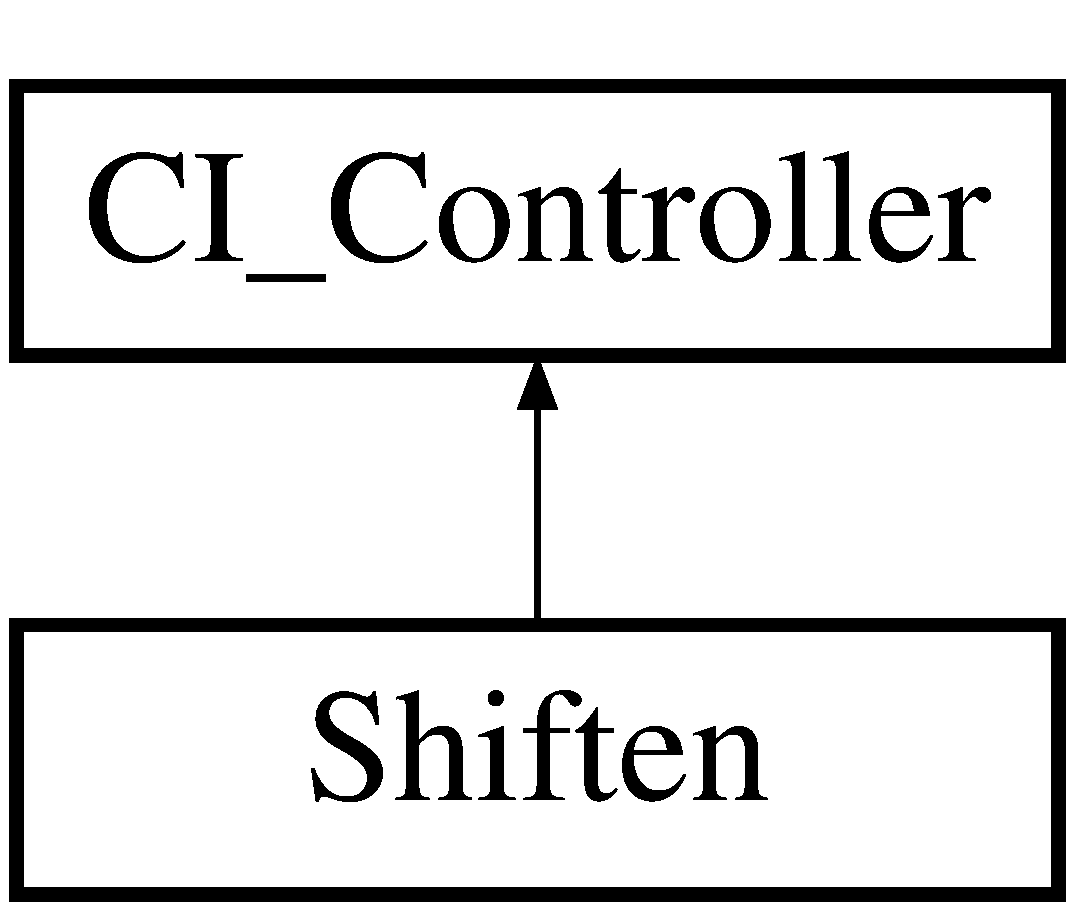
\includegraphics[height=2.000000cm]{class_shiften}
\end{center}
\end{figure}
\subsection*{Public Member Functions}
\begin{DoxyCompactItemize}
\item 
\mbox{\hyperlink{class_shiften_a095c5d389db211932136b53f25f39685}{\+\_\+\+\_\+construct}} ()
\item 
\mbox{\hyperlink{class_shiften_a842e4774e3b3601a005b995c02f7e883}{update}} ()
\begin{DoxyCompactList}\small\item\em Functie voor het aanpassen en aanmaken van shiften. \end{DoxyCompactList}\item 
\mbox{\hyperlink{class_shiften_a2f8258add505482d7f00ea26493a5723}{delete}} (\$id)
\begin{DoxyCompactList}\small\item\em Functie voor het verwijderen van shiften. \end{DoxyCompactList}\item 
\mbox{\hyperlink{class_shiften_ab799250126ff159fd1ca9e896a57bcb6}{vrijwilliger\+In\+Shift\+Toevoegen}} (\$shift\+Id, \$persoon\+Id)
\begin{DoxyCompactList}\small\item\em Functie voor het toevoegen van een vrijwilliger in een shift. \end{DoxyCompactList}\item 
\mbox{\hyperlink{class_shiften_acd0ea5b1f1b5ef6ee363916d98a261cb}{vrijwilliger\+In\+Shift\+Verwijderen}} (\$shift\+Id, \$persoon\+Id)
\begin{DoxyCompactList}\small\item\em Functie voor het verwijderen van een vrijwilliger uit een shift. \end{DoxyCompactList}\item 
\mbox{\hyperlink{class_shiften_acc7f0b07717791306d83399416669ef9}{vrijwilliger\+In\+Shift\+Weergeven}} (\$shift\+Id)
\begin{DoxyCompactList}\small\item\em Functie voor het weergeven van alle vrijwilliger van een bepaalde shift. \end{DoxyCompactList}\end{DoxyCompactItemize}


\subsection{Constructor \& Destructor Documentation}
\mbox{\Hypertarget{class_shiften_a095c5d389db211932136b53f25f39685}\label{class_shiften_a095c5d389db211932136b53f25f39685}} 
\index{Shiften@{Shiften}!\+\_\+\+\_\+construct@{\+\_\+\+\_\+construct}}
\index{\+\_\+\+\_\+construct@{\+\_\+\+\_\+construct}!Shiften@{Shiften}}
\subsubsection{\texorpdfstring{\+\_\+\+\_\+construct()}{\_\_construct()}}
{\footnotesize\ttfamily \+\_\+\+\_\+construct (\begin{DoxyParamCaption}{ }\end{DoxyParamCaption})}

=================================================================================================== G\+R\+E\+IF M\+A\+T\+T\+H\+I\+AS Autoload ~\newline
~\newline
 Redirect to home if no session started

=================================================================================================== /\+G\+R\+E\+IF M\+A\+T\+T\+H\+I\+AS 

\subsection{Member Function Documentation}
\mbox{\Hypertarget{class_shiften_a2f8258add505482d7f00ea26493a5723}\label{class_shiften_a2f8258add505482d7f00ea26493a5723}} 
\index{Shiften@{Shiften}!delete@{delete}}
\index{delete@{delete}!Shiften@{Shiften}}
\subsubsection{\texorpdfstring{delete()}{delete()}}
{\footnotesize\ttfamily delete (\begin{DoxyParamCaption}\item[{}]{\$id }\end{DoxyParamCaption})}



Functie voor het verwijderen van shiften. 

Redirect to keuzemogelijkheidbeheer \mbox{\Hypertarget{class_shiften_a842e4774e3b3601a005b995c02f7e883}\label{class_shiften_a842e4774e3b3601a005b995c02f7e883}} 
\index{Shiften@{Shiften}!update@{update}}
\index{update@{update}!Shiften@{Shiften}}
\subsubsection{\texorpdfstring{update()}{update()}}
{\footnotesize\ttfamily update (\begin{DoxyParamCaption}{ }\end{DoxyParamCaption})}



Functie voor het aanpassen en aanmaken van shiften. 

klasse shift aanmaken en initialiseren

Model inladen

Shift toevoegen of aanpassen

Redirect naar taken pagina \mbox{\Hypertarget{class_shiften_ab799250126ff159fd1ca9e896a57bcb6}\label{class_shiften_ab799250126ff159fd1ca9e896a57bcb6}} 
\index{Shiften@{Shiften}!vrijwilliger\+In\+Shift\+Toevoegen@{vrijwilliger\+In\+Shift\+Toevoegen}}
\index{vrijwilliger\+In\+Shift\+Toevoegen@{vrijwilliger\+In\+Shift\+Toevoegen}!Shiften@{Shiften}}
\subsubsection{\texorpdfstring{vrijwilliger\+In\+Shift\+Toevoegen()}{vrijwilligerInShiftToevoegen()}}
{\footnotesize\ttfamily vrijwilliger\+In\+Shift\+Toevoegen (\begin{DoxyParamCaption}\item[{}]{\$shift\+Id,  }\item[{}]{\$persoon\+Id }\end{DoxyParamCaption})}



Functie voor het toevoegen van een vrijwilliger in een shift. 

Laden van de verkregen data in een ajax-\/venster \mbox{\Hypertarget{class_shiften_acd0ea5b1f1b5ef6ee363916d98a261cb}\label{class_shiften_acd0ea5b1f1b5ef6ee363916d98a261cb}} 
\index{Shiften@{Shiften}!vrijwilliger\+In\+Shift\+Verwijderen@{vrijwilliger\+In\+Shift\+Verwijderen}}
\index{vrijwilliger\+In\+Shift\+Verwijderen@{vrijwilliger\+In\+Shift\+Verwijderen}!Shiften@{Shiften}}
\subsubsection{\texorpdfstring{vrijwilliger\+In\+Shift\+Verwijderen()}{vrijwilligerInShiftVerwijderen()}}
{\footnotesize\ttfamily vrijwilliger\+In\+Shift\+Verwijderen (\begin{DoxyParamCaption}\item[{}]{\$shift\+Id,  }\item[{}]{\$persoon\+Id }\end{DoxyParamCaption})}



Functie voor het verwijderen van een vrijwilliger uit een shift. 

Laden van de verkregen data in een ajax-\/venster \mbox{\Hypertarget{class_shiften_acc7f0b07717791306d83399416669ef9}\label{class_shiften_acc7f0b07717791306d83399416669ef9}} 
\index{Shiften@{Shiften}!vrijwilliger\+In\+Shift\+Weergeven@{vrijwilliger\+In\+Shift\+Weergeven}}
\index{vrijwilliger\+In\+Shift\+Weergeven@{vrijwilliger\+In\+Shift\+Weergeven}!Shiften@{Shiften}}
\subsubsection{\texorpdfstring{vrijwilliger\+In\+Shift\+Weergeven()}{vrijwilligerInShiftWeergeven()}}
{\footnotesize\ttfamily vrijwilliger\+In\+Shift\+Weergeven (\begin{DoxyParamCaption}\item[{}]{\$shift\+Id }\end{DoxyParamCaption})}



Functie voor het weergeven van alle vrijwilliger van een bepaalde shift. 

Laden van de verkregen data in een ajax-\/venster 

The documentation for this class was generated from the following file\+:\begin{DoxyCompactItemize}
\item 
application/controllers/\mbox{\hyperlink{_shiften_8php}{Shiften.\+php}}\end{DoxyCompactItemize}

\hypertarget{class_shiften___model}{}\section{Shiften\+\_\+\+Model Class Reference}
\label{class_shiften___model}\index{Shiften\+\_\+\+Model@{Shiften\+\_\+\+Model}}
Inheritance diagram for Shiften\+\_\+\+Model\+:\begin{figure}[H]
\begin{center}
\leavevmode
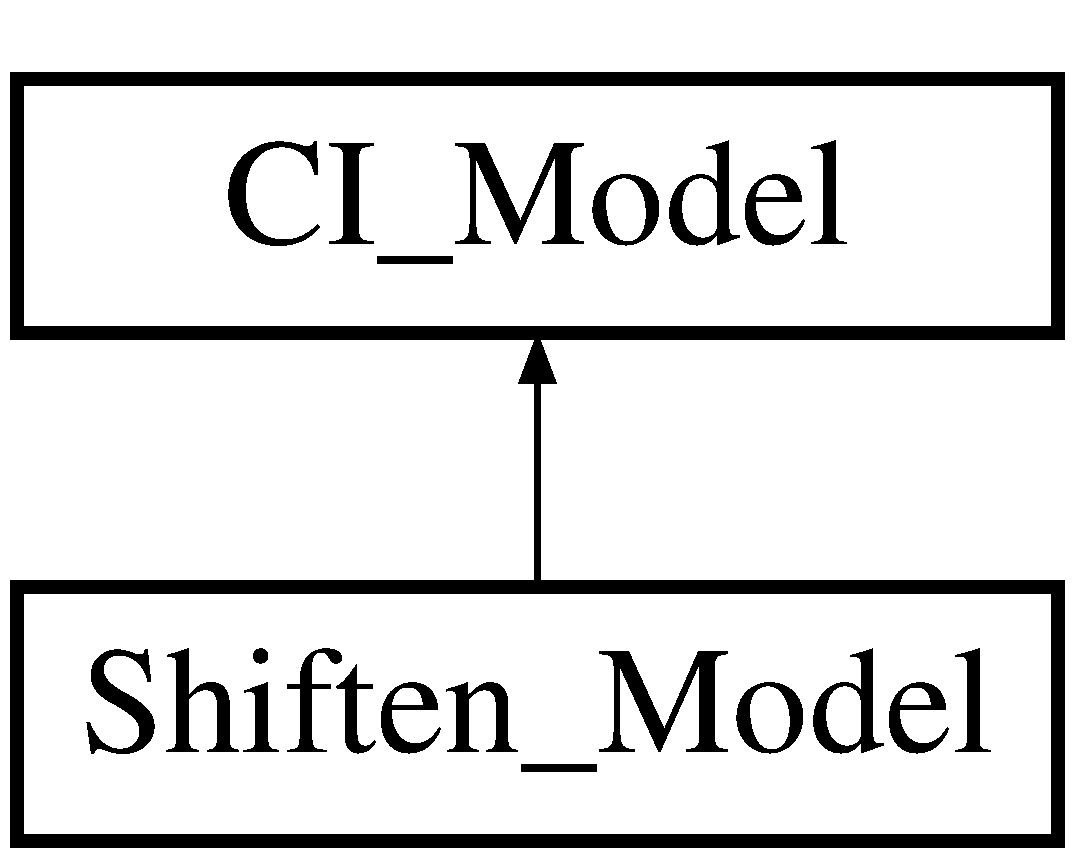
\includegraphics[height=2.000000cm]{class_shiften___model}
\end{center}
\end{figure}
\subsection*{Public Member Functions}
\begin{DoxyCompactItemize}
\item 
\mbox{\hyperlink{class_shiften___model_a0e222557a11630559c7eaa6ca29c55a6}{get\+\_\+by\+Id}} (\$id)
\item 
\mbox{\Hypertarget{class_shiften___model_aad336432fa42862a23f7c8b772e46f64}\label{class_shiften___model_aad336432fa42862a23f7c8b772e46f64}} 
\mbox{\hyperlink{class_shiften___model_aad336432fa42862a23f7c8b772e46f64}{get\+All\+By\+Naam}} ()
\begin{DoxyCompactList}\small\item\em Functie voor het ophalen van alle shiften gesorteerd op basis van naam. \end{DoxyCompactList}\item 
\mbox{\hyperlink{class_shiften___model_a23921f9ceba4ae6768237864469d1cf5}{get\+All\+By\+Naam\+Where\+Taak\+Id}} (\$id)
\item 
\mbox{\hyperlink{class_shiften___model_af5e1c7d324bab167ecaa3e827161ec13}{update}} (\$shift)
\item 
\mbox{\hyperlink{class_shiften___model_ae95a20c13c92700b673c4b850a084b85}{add}} (\$shift)
\item 
\mbox{\hyperlink{class_shiften___model_aa8ebb0f37babc9dbfc4c026f0a73d6e6}{delete}} (\$id)
\end{DoxyCompactItemize}


\subsection{Detailed Description}
T\+IM S\+W\+E\+R\+TS L\+A\+ST U\+P\+D\+A\+T\+ED\+: 18 03 30 \mbox{\hyperlink{class_shiften}{Shiften}} M\+O\+D\+EL

Model voor het beheren van de tabel shiften in de database 

\subsection{Member Function Documentation}
\mbox{\Hypertarget{class_shiften___model_ae95a20c13c92700b673c4b850a084b85}\label{class_shiften___model_ae95a20c13c92700b673c4b850a084b85}} 
\index{Shiften\+\_\+\+Model@{Shiften\+\_\+\+Model}!add@{add}}
\index{add@{add}!Shiften\+\_\+\+Model@{Shiften\+\_\+\+Model}}
\subsubsection{\texorpdfstring{add()}{add()}}
{\footnotesize\ttfamily Shiften\+\_\+\+Model\+::add (\begin{DoxyParamCaption}\item[{}]{\$shift }\end{DoxyParamCaption})}

Functie voor het tevoegen van een welbepaalde shift die meegegeven wordt als object. 
\begin{DoxyParams}[1]{Parameters}
std\+Class & {\em \$shift} & Object van een shift die toegevoegd moet worden \\
\hline
\end{DoxyParams}
\mbox{\Hypertarget{class_shiften___model_aa8ebb0f37babc9dbfc4c026f0a73d6e6}\label{class_shiften___model_aa8ebb0f37babc9dbfc4c026f0a73d6e6}} 
\index{Shiften\+\_\+\+Model@{Shiften\+\_\+\+Model}!delete@{delete}}
\index{delete@{delete}!Shiften\+\_\+\+Model@{Shiften\+\_\+\+Model}}
\subsubsection{\texorpdfstring{delete()}{delete()}}
{\footnotesize\ttfamily Shiften\+\_\+\+Model\+::delete (\begin{DoxyParamCaption}\item[{}]{\$id }\end{DoxyParamCaption})}

Functie voor het verwijderen van een welbepaalde shift waarvan de id meegegeven word. 
\begin{DoxyParams}[1]{Parameters}
string & {\em \$id} & Id van de shift de verwijderd moet worden \\
\hline
\end{DoxyParams}
\mbox{\Hypertarget{class_shiften___model_a0e222557a11630559c7eaa6ca29c55a6}\label{class_shiften___model_a0e222557a11630559c7eaa6ca29c55a6}} 
\index{Shiften\+\_\+\+Model@{Shiften\+\_\+\+Model}!get\+\_\+by\+Id@{get\+\_\+by\+Id}}
\index{get\+\_\+by\+Id@{get\+\_\+by\+Id}!Shiften\+\_\+\+Model@{Shiften\+\_\+\+Model}}
\subsubsection{\texorpdfstring{get\+\_\+by\+Id()}{get\_byId()}}
{\footnotesize\ttfamily Shiften\+\_\+\+Model\+::get\+\_\+by\+Id (\begin{DoxyParamCaption}\item[{}]{\$id }\end{DoxyParamCaption})}

Functie voor het ophalen van een specifieke shift op basis van een id. 
\begin{DoxyParams}[1]{Parameters}
string & {\em \$id} & Id van de shift \\
\hline
\end{DoxyParams}
\mbox{\Hypertarget{class_shiften___model_a23921f9ceba4ae6768237864469d1cf5}\label{class_shiften___model_a23921f9ceba4ae6768237864469d1cf5}} 
\index{Shiften\+\_\+\+Model@{Shiften\+\_\+\+Model}!get\+All\+By\+Naam\+Where\+Taak\+Id@{get\+All\+By\+Naam\+Where\+Taak\+Id}}
\index{get\+All\+By\+Naam\+Where\+Taak\+Id@{get\+All\+By\+Naam\+Where\+Taak\+Id}!Shiften\+\_\+\+Model@{Shiften\+\_\+\+Model}}
\subsubsection{\texorpdfstring{get\+All\+By\+Naam\+Where\+Taak\+Id()}{getAllByNaamWhereTaakId()}}
{\footnotesize\ttfamily Shiften\+\_\+\+Model\+::get\+All\+By\+Naam\+Where\+Taak\+Id (\begin{DoxyParamCaption}\item[{}]{\$id }\end{DoxyParamCaption})}

Functie voor het ophalen van alle shiften die bij een specifieke taak horen. Alle gevonden shiften worden gesorteerd op basis van naam. 
\begin{DoxyParams}[1]{Parameters}
string & {\em \$id} & Id van de taak \\
\hline
\end{DoxyParams}
\mbox{\Hypertarget{class_shiften___model_af5e1c7d324bab167ecaa3e827161ec13}\label{class_shiften___model_af5e1c7d324bab167ecaa3e827161ec13}} 
\index{Shiften\+\_\+\+Model@{Shiften\+\_\+\+Model}!update@{update}}
\index{update@{update}!Shiften\+\_\+\+Model@{Shiften\+\_\+\+Model}}
\subsubsection{\texorpdfstring{update()}{update()}}
{\footnotesize\ttfamily Shiften\+\_\+\+Model\+::update (\begin{DoxyParamCaption}\item[{}]{\$shift }\end{DoxyParamCaption})}

Functie voor het aanpassen van een welbepaalde shift die meegegeven wordt als object. 
\begin{DoxyParams}[1]{Parameters}
std\+Class & {\em \$shift} & Object van een shift die aangepast moet worden \\
\hline
\end{DoxyParams}


The documentation for this class was generated from the following file\+:\begin{DoxyCompactItemize}
\item 
application/models/Shiften\+\_\+model.\+php\end{DoxyCompactItemize}

\hypertarget{class_soort__model}{}\section{Soort\+\_\+model Class Reference}
\label{class_soort__model}\index{Soort\+\_\+model@{Soort\+\_\+model}}
Inheritance diagram for Soort\+\_\+model\+:\begin{figure}[H]
\begin{center}
\leavevmode
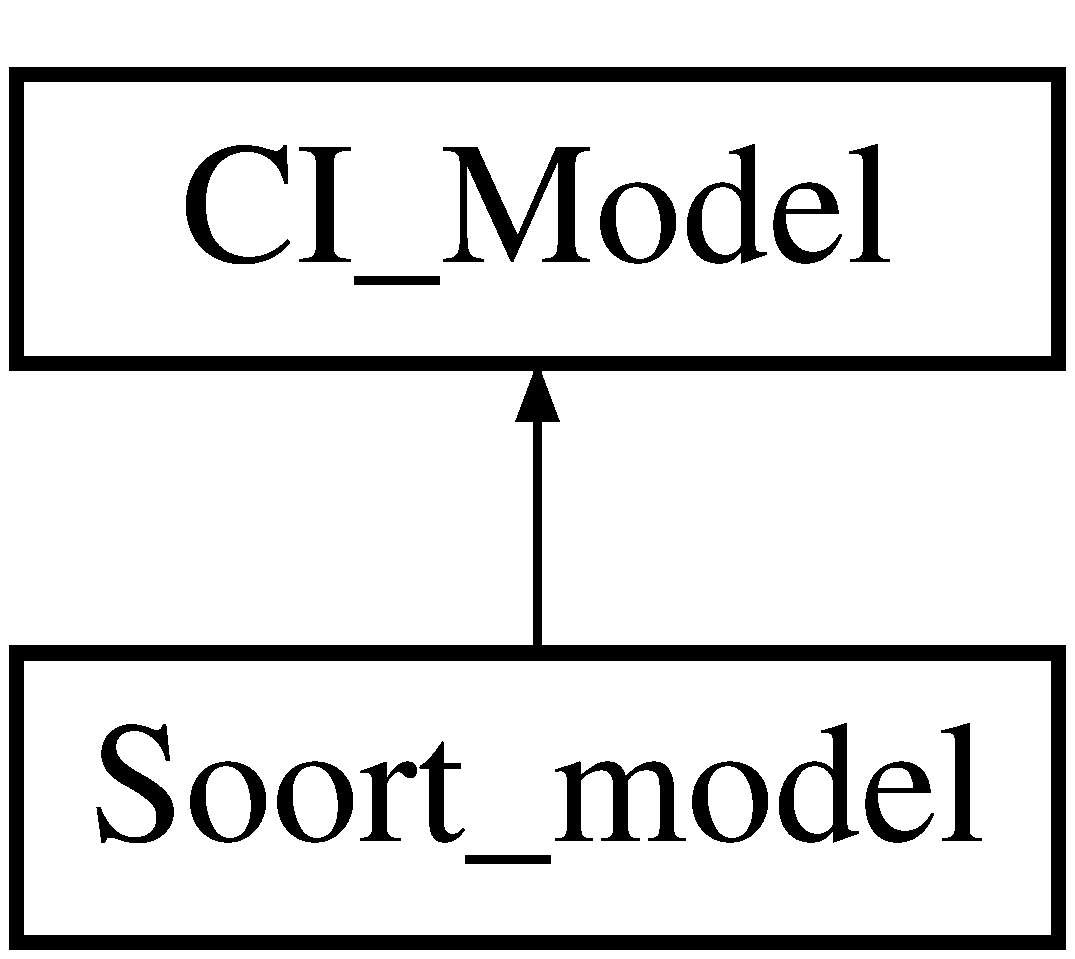
\includegraphics[height=2.000000cm]{class_soort__model}
\end{center}
\end{figure}
\subsection*{Public Member Functions}
\begin{DoxyCompactItemize}
\item 
\mbox{\Hypertarget{class_soort__model_a28a2efaf8d40808d5567d7972ba75ca0}\label{class_soort__model_a28a2efaf8d40808d5567d7972ba75ca0}} 
{\bfseries get\+\_\+by\+Id} (\$id, \$token)
\item 
\mbox{\Hypertarget{class_soort__model_af7ccb69058c9250e64e9c11046349e26}\label{class_soort__model_af7ccb69058c9250e64e9c11046349e26}} 
{\bfseries get\+All} (\$id)
\end{DoxyCompactItemize}


The documentation for this class was generated from the following file\+:\begin{DoxyCompactItemize}
\item 
application/models/Soort\+\_\+model.\+php\end{DoxyCompactItemize}

\hypertarget{class_taken}{}\section{Taken Class Reference}
\label{class_taken}\index{Taken@{Taken}}
Inheritance diagram for Taken\+:\begin{figure}[H]
\begin{center}
\leavevmode
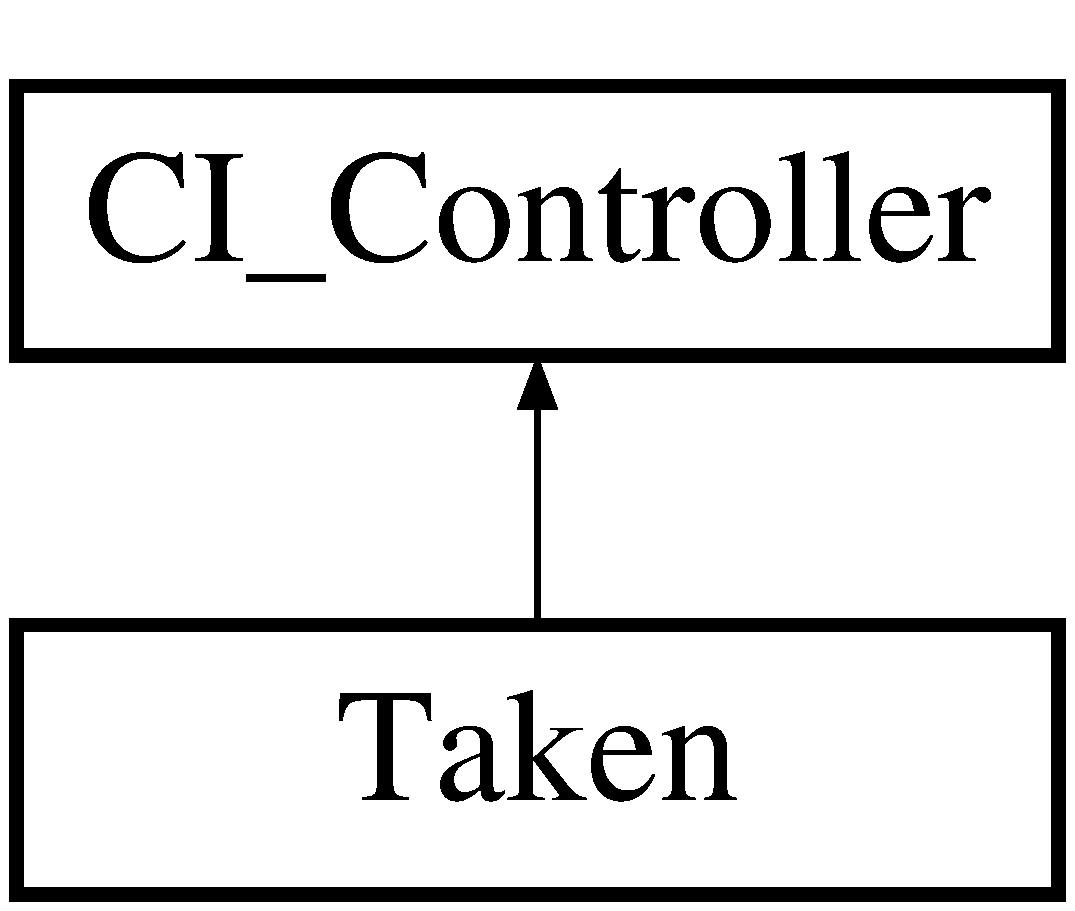
\includegraphics[height=2.000000cm]{class_taken}
\end{center}
\end{figure}
\subsection*{Public Member Functions}
\begin{DoxyCompactItemize}
\item 
\mbox{\Hypertarget{class_taken_a842e4774e3b3601a005b995c02f7e883}\label{class_taken_a842e4774e3b3601a005b995c02f7e883}} 
{\bfseries update} ()
\item 
\mbox{\Hypertarget{class_taken_a2f8258add505482d7f00ea26493a5723}\label{class_taken_a2f8258add505482d7f00ea26493a5723}} 
{\bfseries delete} (\$id)
\end{DoxyCompactItemize}


The documentation for this class was generated from the following file\+:\begin{DoxyCompactItemize}
\item 
application/controllers/Taken.\+php\end{DoxyCompactItemize}

\hypertarget{class_taken___model}{}\section{Taken\+\_\+\+Model Class Reference}
\label{class_taken___model}\index{Taken\+\_\+\+Model@{Taken\+\_\+\+Model}}


Model voor beheren van de tabel taken van de database.  


Inheritance diagram for Taken\+\_\+\+Model\+:\begin{figure}[H]
\begin{center}
\leavevmode
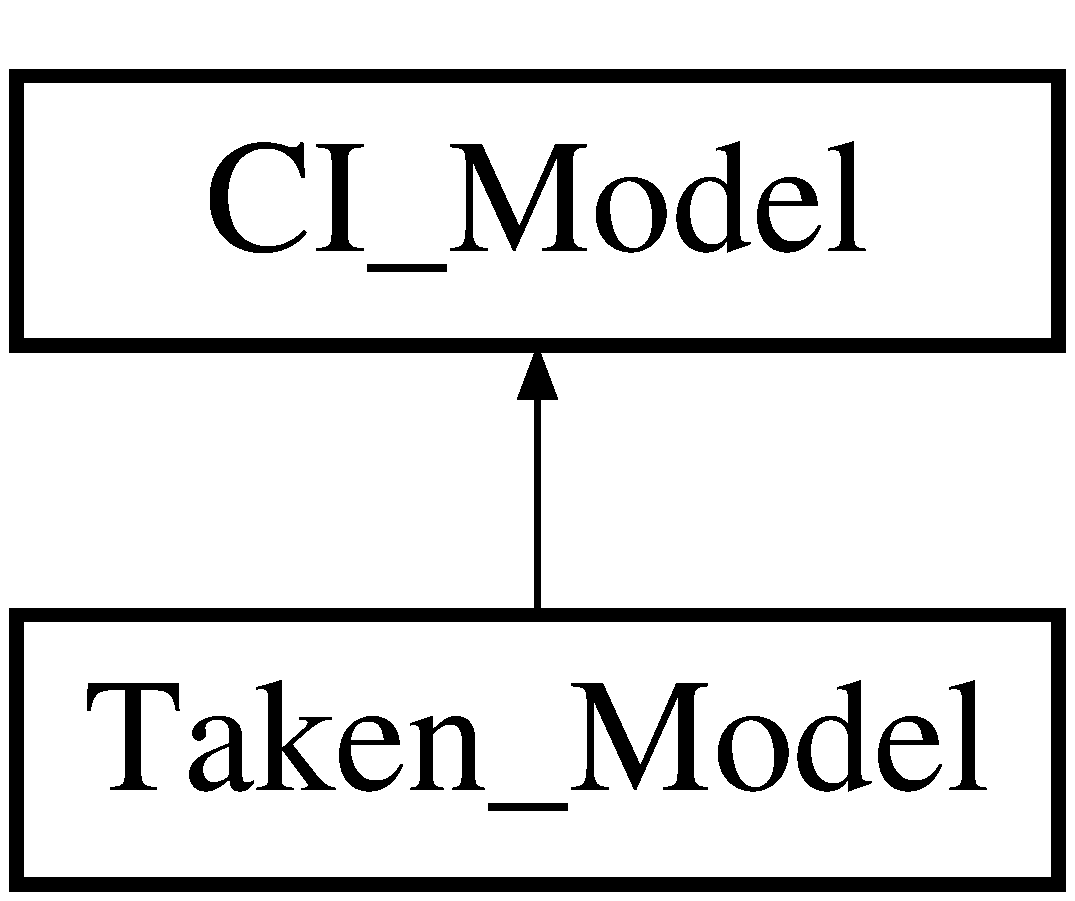
\includegraphics[height=2.000000cm]{class_taken___model}
\end{center}
\end{figure}
\subsection*{Public Member Functions}
\begin{DoxyCompactItemize}
\item 
\mbox{\hyperlink{class_taken___model_ab8c238bca4fc5170294717b94c875cc3}{get\+\_\+by\+Id}} (\$id)
\item 
\mbox{\Hypertarget{class_taken___model_a5e53ebfe17a0adb72cccb12728f83d6a}\label{class_taken___model_a5e53ebfe17a0adb72cccb12728f83d6a}} 
\mbox{\hyperlink{class_taken___model_a5e53ebfe17a0adb72cccb12728f83d6a}{get\+All\+By\+Naam}} ()
\begin{DoxyCompactList}\small\item\em Functie voor het ophalen van alle taken gesorteerd op basis van naam. \end{DoxyCompactList}\item 
\mbox{\hyperlink{class_taken___model_aee432ed4b391407df1bf5d8c4973e5fa}{get\+All\+By\+Naam\+Where\+Keuze\+Mogelijkheid}} (\$id)
\item 
\mbox{\hyperlink{class_taken___model_a1b4e18ac99960b20467b3b3cbaa817b4}{get\+All\+With\+Shiften\+\_\+by\+Keuzemogelijkheid\+Id}} (\$id)
\item 
\mbox{\hyperlink{class_taken___model_ab4e93ac196a1aeb83582faa332619c86}{update}} (\$taak)
\item 
\mbox{\hyperlink{class_taken___model_a4ef6e4ab1c71556c29cdc6549e8c888b}{add}} (\$taak)
\item 
\mbox{\hyperlink{class_taken___model_ab00c14e7a0a268dc3f708b45f3bd172b}{delete}} (\$id)
\end{DoxyCompactItemize}


\subsection{Detailed Description}
Model voor beheren van de tabel taken van de database. 

\subsection{Member Function Documentation}
\mbox{\Hypertarget{class_taken___model_a4ef6e4ab1c71556c29cdc6549e8c888b}\label{class_taken___model_a4ef6e4ab1c71556c29cdc6549e8c888b}} 
\index{Taken\+\_\+\+Model@{Taken\+\_\+\+Model}!add@{add}}
\index{add@{add}!Taken\+\_\+\+Model@{Taken\+\_\+\+Model}}
\subsubsection{\texorpdfstring{add()}{add()}}
{\footnotesize\ttfamily Taken\+\_\+\+Model\+::add (\begin{DoxyParamCaption}\item[{}]{\$taak }\end{DoxyParamCaption})}

Functie voor het toevoegen van een taak die mee wordt geleverd als object. 
\begin{DoxyParams}[1]{Parameters}
std\+Class & {\em \$taak} & Object van de taak die toegevoegd moet worden \\
\hline
\end{DoxyParams}
\mbox{\Hypertarget{class_taken___model_ab00c14e7a0a268dc3f708b45f3bd172b}\label{class_taken___model_ab00c14e7a0a268dc3f708b45f3bd172b}} 
\index{Taken\+\_\+\+Model@{Taken\+\_\+\+Model}!delete@{delete}}
\index{delete@{delete}!Taken\+\_\+\+Model@{Taken\+\_\+\+Model}}
\subsubsection{\texorpdfstring{delete()}{delete()}}
{\footnotesize\ttfamily Taken\+\_\+\+Model\+::delete (\begin{DoxyParamCaption}\item[{}]{\$id }\end{DoxyParamCaption})}

Functie voor het verwijderen van een taak die mee wordt geleverd als id. 
\begin{DoxyParams}[1]{Parameters}
string & {\em \$id} & Id van de taak die verwijderd moet worden \\
\hline
\end{DoxyParams}
\mbox{\Hypertarget{class_taken___model_ab8c238bca4fc5170294717b94c875cc3}\label{class_taken___model_ab8c238bca4fc5170294717b94c875cc3}} 
\index{Taken\+\_\+\+Model@{Taken\+\_\+\+Model}!get\+\_\+by\+Id@{get\+\_\+by\+Id}}
\index{get\+\_\+by\+Id@{get\+\_\+by\+Id}!Taken\+\_\+\+Model@{Taken\+\_\+\+Model}}
\subsubsection{\texorpdfstring{get\+\_\+by\+Id()}{get\_byId()}}
{\footnotesize\ttfamily Taken\+\_\+\+Model\+::get\+\_\+by\+Id (\begin{DoxyParamCaption}\item[{}]{\$id }\end{DoxyParamCaption})}

Functie voor het opvragen van een specifieke taak. 
\begin{DoxyParams}[1]{Parameters}
string & {\em \$id} & Id van de taak \\
\hline
\end{DoxyParams}
\mbox{\Hypertarget{class_taken___model_aee432ed4b391407df1bf5d8c4973e5fa}\label{class_taken___model_aee432ed4b391407df1bf5d8c4973e5fa}} 
\index{Taken\+\_\+\+Model@{Taken\+\_\+\+Model}!get\+All\+By\+Naam\+Where\+Keuze\+Mogelijkheid@{get\+All\+By\+Naam\+Where\+Keuze\+Mogelijkheid}}
\index{get\+All\+By\+Naam\+Where\+Keuze\+Mogelijkheid@{get\+All\+By\+Naam\+Where\+Keuze\+Mogelijkheid}!Taken\+\_\+\+Model@{Taken\+\_\+\+Model}}
\subsubsection{\texorpdfstring{get\+All\+By\+Naam\+Where\+Keuze\+Mogelijkheid()}{getAllByNaamWhereKeuzeMogelijkheid()}}
{\footnotesize\ttfamily Taken\+\_\+\+Model\+::get\+All\+By\+Naam\+Where\+Keuze\+Mogelijkheid (\begin{DoxyParamCaption}\item[{}]{\$id }\end{DoxyParamCaption})}

Functie voor ophalen van alle taken die behoren tot een welbepaalde keuzemogelijkheid. 
\begin{DoxyParams}[1]{Parameters}
string & {\em \$id} & Id van de keuzemogelijkheid \\
\hline
\end{DoxyParams}
\mbox{\Hypertarget{class_taken___model_a1b4e18ac99960b20467b3b3cbaa817b4}\label{class_taken___model_a1b4e18ac99960b20467b3b3cbaa817b4}} 
\index{Taken\+\_\+\+Model@{Taken\+\_\+\+Model}!get\+All\+With\+Shiften\+\_\+by\+Keuzemogelijkheid\+Id@{get\+All\+With\+Shiften\+\_\+by\+Keuzemogelijkheid\+Id}}
\index{get\+All\+With\+Shiften\+\_\+by\+Keuzemogelijkheid\+Id@{get\+All\+With\+Shiften\+\_\+by\+Keuzemogelijkheid\+Id}!Taken\+\_\+\+Model@{Taken\+\_\+\+Model}}
\subsubsection{\texorpdfstring{get\+All\+With\+Shiften\+\_\+by\+Keuzemogelijkheid\+Id()}{getAllWithShiften\_byKeuzemogelijkheidId()}}
{\footnotesize\ttfamily Taken\+\_\+\+Model\+::get\+All\+With\+Shiften\+\_\+by\+Keuzemogelijkheid\+Id (\begin{DoxyParamCaption}\item[{}]{\$id }\end{DoxyParamCaption})}

Functie voor het ophalen van alle shiften die tot een taak behoren met een specifieke keuzemogelijkheid. 
\begin{DoxyParams}[1]{Parameters}
string & {\em \$id} & Id van de taak \\
\hline
\end{DoxyParams}
Ga alle taken ophalen onder een bepaalde keuzemgelijkheid

Ga alle shiften ophalen onder een bepaalde taak \mbox{\Hypertarget{class_taken___model_ab4e93ac196a1aeb83582faa332619c86}\label{class_taken___model_ab4e93ac196a1aeb83582faa332619c86}} 
\index{Taken\+\_\+\+Model@{Taken\+\_\+\+Model}!update@{update}}
\index{update@{update}!Taken\+\_\+\+Model@{Taken\+\_\+\+Model}}
\subsubsection{\texorpdfstring{update()}{update()}}
{\footnotesize\ttfamily Taken\+\_\+\+Model\+::update (\begin{DoxyParamCaption}\item[{}]{\$taak }\end{DoxyParamCaption})}

Functie voor het aanpassen van een taak die mee wordt geleverd als object. 
\begin{DoxyParams}[1]{Parameters}
std\+Class & {\em \$taak} & Object van de taak die aangepast moet worden \\
\hline
\end{DoxyParams}


The documentation for this class was generated from the following file\+:\begin{DoxyCompactItemize}
\item 
E\+:/\+D\+R\+I\+V\+E/\+C\+O\+L\+L\+E\+G\+E/\+T\+M/\+P0202/\+K\+P0201/\+R\+E\+P\+O/application/models/Taken\+\_\+model.\+php\end{DoxyCompactItemize}

\hypertarget{class_vervoerswijze__model}{}\section{Vervoerswijze\+\_\+model Class Reference}
\label{class_vervoerswijze__model}\index{Vervoerswijze\+\_\+model@{Vervoerswijze\+\_\+model}}
Inheritance diagram for Vervoerswijze\+\_\+model\+:\begin{figure}[H]
\begin{center}
\leavevmode
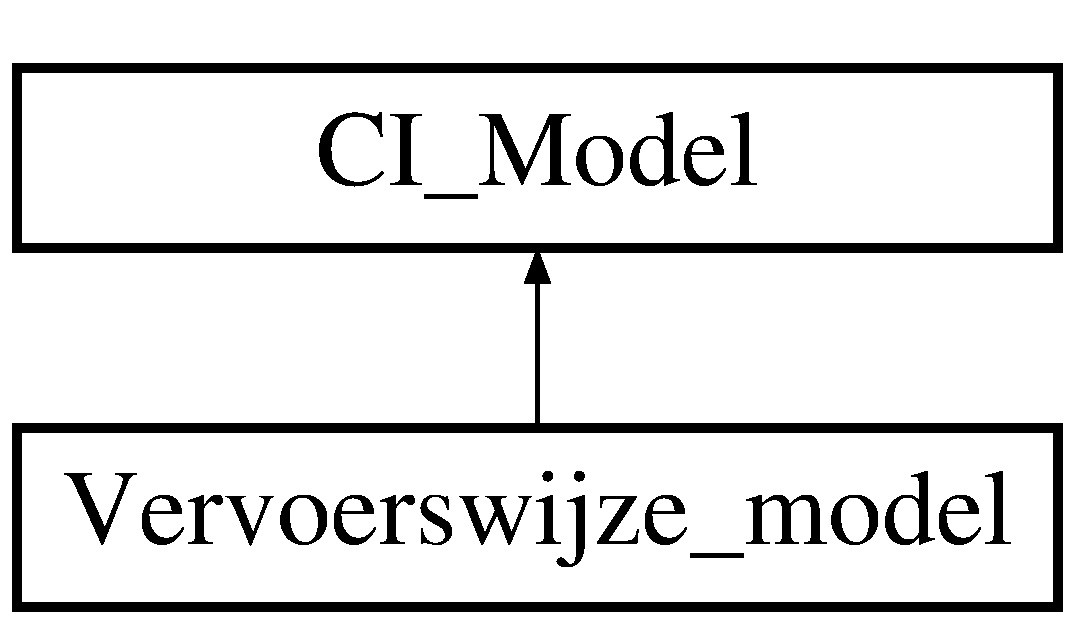
\includegraphics[height=2.000000cm]{class_vervoerswijze__model}
\end{center}
\end{figure}


The documentation for this class was generated from the following file\+:\begin{DoxyCompactItemize}
\item 
application/models/Vervoerswijze\+\_\+model.\+php\end{DoxyCompactItemize}

\hypertarget{class_vrijwilliger}{}\section{Vrijwilliger Class Reference}
\label{class_vrijwilliger}\index{Vrijwilliger@{Vrijwilliger}}


Controller voor vrijwilligersfunctionaliteiten.  


Inheritance diagram for Vrijwilliger\+:\begin{figure}[H]
\begin{center}
\leavevmode
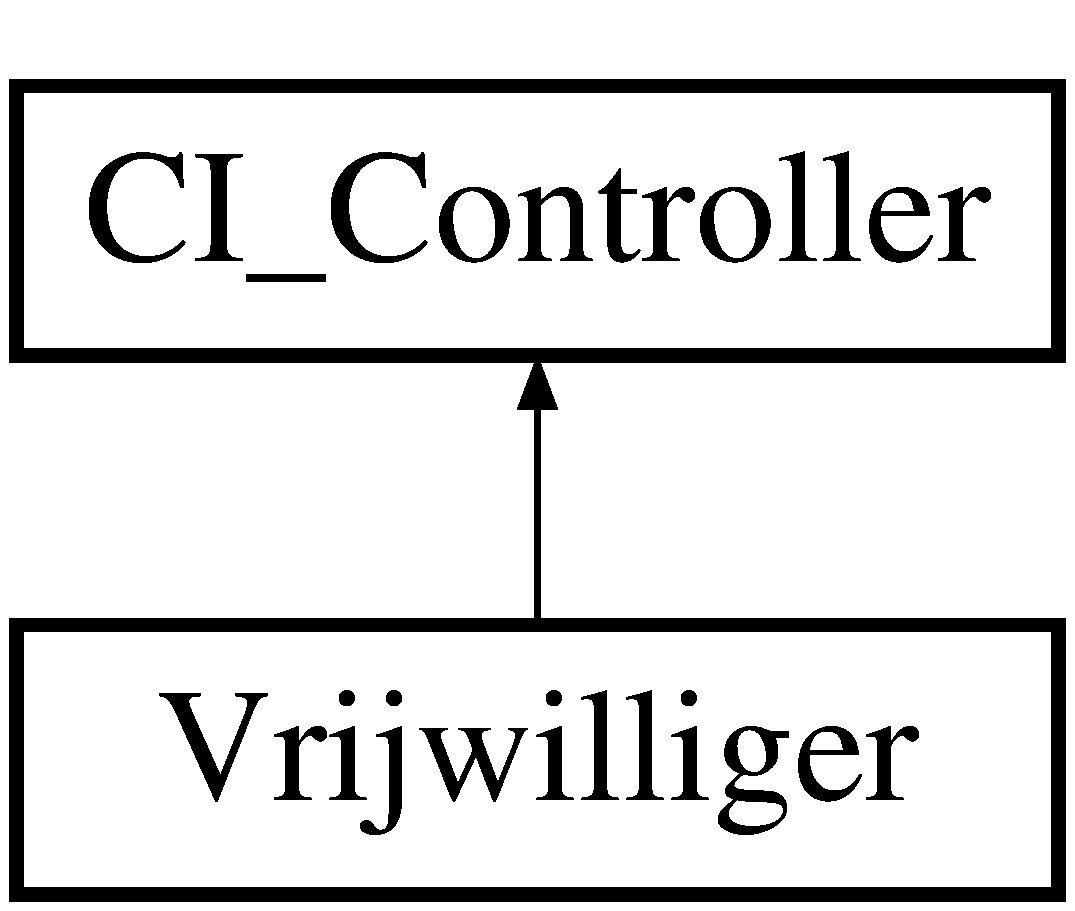
\includegraphics[height=2.000000cm]{class_vrijwilliger}
\end{center}
\end{figure}
\subsection*{Public Member Functions}
\begin{DoxyCompactItemize}
\item 
\mbox{\hyperlink{class_vrijwilliger_af515ff61252b881037a1c5a8fc3b320a}{\+\_\+\+\_\+construct}} ()
\item 
\mbox{\hyperlink{class_vrijwilliger_aa58c80ff70c366f67133c3ad1d0f40b5}{dash}} (\$view=null, \$extras=null)
\item 
\mbox{\hyperlink{class_vrijwilliger_aced009dfd83a274ae5e079f753502d55}{logout}} ()
\end{DoxyCompactItemize}


\subsection{Detailed Description}
Controller voor vrijwilligersfunctionaliteiten. 

\subsection{Constructor \& Destructor Documentation}
\mbox{\Hypertarget{class_vrijwilliger_af515ff61252b881037a1c5a8fc3b320a}\label{class_vrijwilliger_af515ff61252b881037a1c5a8fc3b320a}} 
\index{Vrijwilliger@{Vrijwilliger}!\+\_\+\+\_\+construct@{\+\_\+\+\_\+construct}}
\index{\+\_\+\+\_\+construct@{\+\_\+\+\_\+construct}!Vrijwilliger@{Vrijwilliger}}
\subsubsection{\texorpdfstring{\+\_\+\+\_\+construct()}{\_\_construct()}}
{\footnotesize\ttfamily Vrijwilliger\+::\+\_\+\+\_\+construct (\begin{DoxyParamCaption}{ }\end{DoxyParamCaption})}

Default Contstructor 

\subsection{Member Function Documentation}
\mbox{\Hypertarget{class_vrijwilliger_aa58c80ff70c366f67133c3ad1d0f40b5}\label{class_vrijwilliger_aa58c80ff70c366f67133c3ad1d0f40b5}} 
\index{Vrijwilliger@{Vrijwilliger}!dash@{dash}}
\index{dash@{dash}!Vrijwilliger@{Vrijwilliger}}
\subsubsection{\texorpdfstring{dash()}{dash()}}
{\footnotesize\ttfamily Vrijwilliger\+::dash (\begin{DoxyParamCaption}\item[{}]{\$view = {\ttfamily null},  }\item[{}]{\$extras = {\ttfamily null} }\end{DoxyParamCaption})}

Container voor alle dashbord schermen van vrijwilliger 
\begin{DoxyParams}[1]{Parameters}
string & {\em \$view} & Scherm dat opgeroepen word in het dashbord van administrator \\
\hline
string & {\em \$extras} & Optionele parameters \\
\hline
\end{DoxyParams}
\mbox{\Hypertarget{class_vrijwilliger_aced009dfd83a274ae5e079f753502d55}\label{class_vrijwilliger_aced009dfd83a274ae5e079f753502d55}} 
\index{Vrijwilliger@{Vrijwilliger}!logout@{logout}}
\index{logout@{logout}!Vrijwilliger@{Vrijwilliger}}
\subsubsection{\texorpdfstring{logout()}{logout()}}
{\footnotesize\ttfamily Vrijwilliger\+::logout (\begin{DoxyParamCaption}{ }\end{DoxyParamCaption})}

Meld vrijwilliger af 

The documentation for this class was generated from the following file\+:\begin{DoxyCompactItemize}
\item 
E\+:/\+D\+R\+I\+V\+E/\+C\+O\+L\+L\+E\+G\+E/\+T\+M/\+P0202/\+K\+P0201/\+R\+E\+P\+O/application/controllers/Vrijwilliger.\+php\end{DoxyCompactItemize}

\hypertarget{class_vrijwilligers_in_shift___model}{}\section{Vrijwilligers\+In\+Shift\+\_\+\+Model Class Reference}
\label{class_vrijwilligers_in_shift___model}\index{Vrijwilligers\+In\+Shift\+\_\+\+Model@{Vrijwilligers\+In\+Shift\+\_\+\+Model}}


Model voor beheren van de tabel shift van de database.  


Inheritance diagram for Vrijwilligers\+In\+Shift\+\_\+\+Model\+:\begin{figure}[H]
\begin{center}
\leavevmode
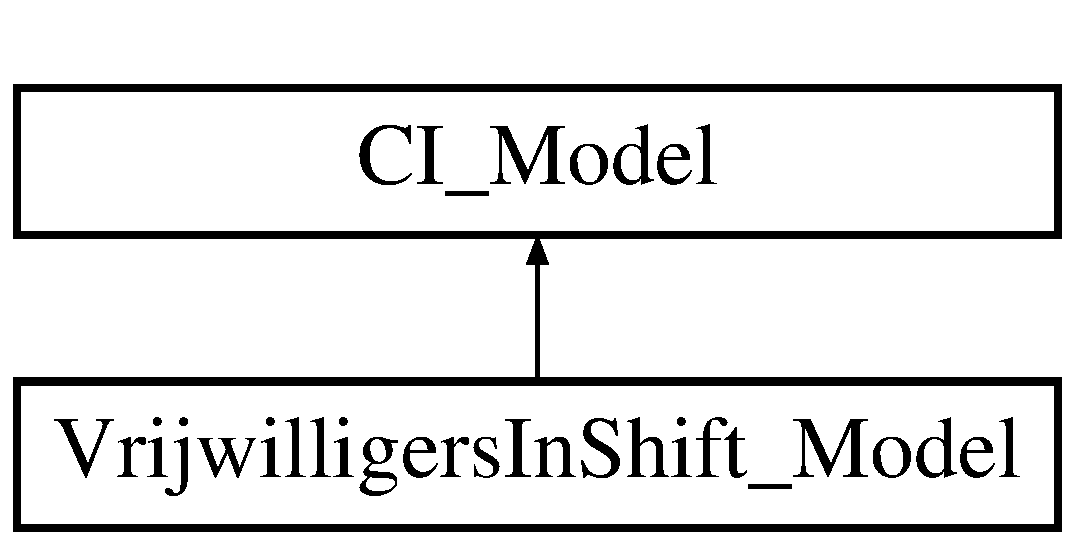
\includegraphics[height=2.000000cm]{class_vrijwilligers_in_shift___model}
\end{center}
\end{figure}
\subsection*{Public Member Functions}
\begin{DoxyCompactItemize}
\item 
\mbox{\hyperlink{class_vrijwilligers_in_shift___model_ac7afbe51273364c55dd352b3c9554592}{get\+\_\+by\+Shift\+Id}} (\$id)
\item 
\mbox{\hyperlink{class_vrijwilligers_in_shift___model_a8a9b3e545063a3b69d118ac1109b3da4}{get\+All\+By\+Shift\+Id}} (\$shift\+Id)
\item 
\mbox{\hyperlink{class_vrijwilligers_in_shift___model_aae12e5673029c5081662fa51503c4413}{get\+\_\+by\+Persoon\+Id}} (\$id)
\item 
\mbox{\Hypertarget{class_vrijwilligers_in_shift___model_a8323f4be7e1a03445c0b6c46ede8d35c}\label{class_vrijwilligers_in_shift___model_a8323f4be7e1a03445c0b6c46ede8d35c}} 
\mbox{\hyperlink{class_vrijwilligers_in_shift___model_a8323f4be7e1a03445c0b6c46ede8d35c}{get\+All}} ()
\begin{DoxyCompactList}\small\item\em Functie voor het ophalen van alle vrijwilligers. \end{DoxyCompactList}\item 
\mbox{\hyperlink{class_vrijwilligers_in_shift___model_ace0abb83991ff90729515c3e86c0a3ac}{add}} (\$Vrijwilliger\+In\+Shift)
\item 
\mbox{\hyperlink{class_vrijwilligers_in_shift___model_a62d1d1920e3c5a73f117ad9293260d67}{delete}} (\$shift\+Id, \$persoon\+Id)
\end{DoxyCompactItemize}


\subsection{Detailed Description}
Model voor beheren van de tabel shift van de database. 

\subsection{Member Function Documentation}
\mbox{\Hypertarget{class_vrijwilligers_in_shift___model_ace0abb83991ff90729515c3e86c0a3ac}\label{class_vrijwilligers_in_shift___model_ace0abb83991ff90729515c3e86c0a3ac}} 
\index{Vrijwilligers\+In\+Shift\+\_\+\+Model@{Vrijwilligers\+In\+Shift\+\_\+\+Model}!add@{add}}
\index{add@{add}!Vrijwilligers\+In\+Shift\+\_\+\+Model@{Vrijwilligers\+In\+Shift\+\_\+\+Model}}
\subsubsection{\texorpdfstring{add()}{add()}}
{\footnotesize\ttfamily Vrijwilligers\+In\+Shift\+\_\+\+Model\+::add (\begin{DoxyParamCaption}\item[{}]{\$\+Vrijwilliger\+In\+Shift }\end{DoxyParamCaption})}

Functie voor het toevoegen van een specifieke vrijwilliger voor een specifieke shift. 
\begin{DoxyParams}[1]{Parameters}
std\+Class & {\em \$\+Vrijwilliger\+In\+Shift} & Object met data over de vrijwilliger en de shift. \\
\hline
\end{DoxyParams}
\mbox{\Hypertarget{class_vrijwilligers_in_shift___model_a62d1d1920e3c5a73f117ad9293260d67}\label{class_vrijwilligers_in_shift___model_a62d1d1920e3c5a73f117ad9293260d67}} 
\index{Vrijwilligers\+In\+Shift\+\_\+\+Model@{Vrijwilligers\+In\+Shift\+\_\+\+Model}!delete@{delete}}
\index{delete@{delete}!Vrijwilligers\+In\+Shift\+\_\+\+Model@{Vrijwilligers\+In\+Shift\+\_\+\+Model}}
\subsubsection{\texorpdfstring{delete()}{delete()}}
{\footnotesize\ttfamily Vrijwilligers\+In\+Shift\+\_\+\+Model\+::delete (\begin{DoxyParamCaption}\item[{}]{\$shift\+Id,  }\item[{}]{\$persoon\+Id }\end{DoxyParamCaption})}

Functie voor het verwijderen van een specifieke vrijwilligers voor een specifieke shift. 
\begin{DoxyParams}[1]{Parameters}
string & {\em \$shift\+Id} & \\
\hline
string & {\em \$persoon\+Id} & \\
\hline
\end{DoxyParams}
\mbox{\Hypertarget{class_vrijwilligers_in_shift___model_aae12e5673029c5081662fa51503c4413}\label{class_vrijwilligers_in_shift___model_aae12e5673029c5081662fa51503c4413}} 
\index{Vrijwilligers\+In\+Shift\+\_\+\+Model@{Vrijwilligers\+In\+Shift\+\_\+\+Model}!get\+\_\+by\+Persoon\+Id@{get\+\_\+by\+Persoon\+Id}}
\index{get\+\_\+by\+Persoon\+Id@{get\+\_\+by\+Persoon\+Id}!Vrijwilligers\+In\+Shift\+\_\+\+Model@{Vrijwilligers\+In\+Shift\+\_\+\+Model}}
\subsubsection{\texorpdfstring{get\+\_\+by\+Persoon\+Id()}{get\_byPersoonId()}}
{\footnotesize\ttfamily Vrijwilligers\+In\+Shift\+\_\+\+Model\+::get\+\_\+by\+Persoon\+Id (\begin{DoxyParamCaption}\item[{}]{\$id }\end{DoxyParamCaption})}

Functie voor het ophalen van alle shiften voor een specifieke persoon. 
\begin{DoxyParams}[1]{Parameters}
string & {\em \$id} & Id van de persoon \\
\hline
\end{DoxyParams}
\mbox{\Hypertarget{class_vrijwilligers_in_shift___model_ac7afbe51273364c55dd352b3c9554592}\label{class_vrijwilligers_in_shift___model_ac7afbe51273364c55dd352b3c9554592}} 
\index{Vrijwilligers\+In\+Shift\+\_\+\+Model@{Vrijwilligers\+In\+Shift\+\_\+\+Model}!get\+\_\+by\+Shift\+Id@{get\+\_\+by\+Shift\+Id}}
\index{get\+\_\+by\+Shift\+Id@{get\+\_\+by\+Shift\+Id}!Vrijwilligers\+In\+Shift\+\_\+\+Model@{Vrijwilligers\+In\+Shift\+\_\+\+Model}}
\subsubsection{\texorpdfstring{get\+\_\+by\+Shift\+Id()}{get\_byShiftId()}}
{\footnotesize\ttfamily Vrijwilligers\+In\+Shift\+\_\+\+Model\+::get\+\_\+by\+Shift\+Id (\begin{DoxyParamCaption}\item[{}]{\$id }\end{DoxyParamCaption})}

Functie voor het opvragen van een alle vrijwilliger bij een specifieke shift shift. 
\begin{DoxyParams}[1]{Parameters}
string & {\em \$id} & Id van de shift \\
\hline
\end{DoxyParams}
\mbox{\Hypertarget{class_vrijwilligers_in_shift___model_a8a9b3e545063a3b69d118ac1109b3da4}\label{class_vrijwilligers_in_shift___model_a8a9b3e545063a3b69d118ac1109b3da4}} 
\index{Vrijwilligers\+In\+Shift\+\_\+\+Model@{Vrijwilligers\+In\+Shift\+\_\+\+Model}!get\+All\+By\+Shift\+Id@{get\+All\+By\+Shift\+Id}}
\index{get\+All\+By\+Shift\+Id@{get\+All\+By\+Shift\+Id}!Vrijwilligers\+In\+Shift\+\_\+\+Model@{Vrijwilligers\+In\+Shift\+\_\+\+Model}}
\subsubsection{\texorpdfstring{get\+All\+By\+Shift\+Id()}{getAllByShiftId()}}
{\footnotesize\ttfamily Vrijwilligers\+In\+Shift\+\_\+\+Model\+::get\+All\+By\+Shift\+Id (\begin{DoxyParamCaption}\item[{}]{\$shift\+Id }\end{DoxyParamCaption})}

Functie voor het ophalen van alle vrijwilligers voor een specifieke shift. 
\begin{DoxyParams}[1]{Parameters}
string & {\em \$shift\+Id} & Id van de shift \\
\hline
\end{DoxyParams}


The documentation for this class was generated from the following file\+:\begin{DoxyCompactItemize}
\item 
application/models/Vrijwilligers\+In\+Shift\+\_\+model.\+php\end{DoxyCompactItemize}

\chapter{File Documentation}
\hypertarget{_admin_8php}{}\section{application/controllers/\+Admin.php File Reference}
\label{_admin_8php}\index{application/controllers/\+Admin.\+php@{application/controllers/\+Admin.\+php}}
\subsection*{Data Structures}
\begin{DoxyCompactItemize}
\item 
class \mbox{\hyperlink{class_admin}{Admin}}
\end{DoxyCompactItemize}

\hypertarget{_deelnemer_8php}{}\section{application/controllers/\+Deelnemer.php File Reference}
\label{_deelnemer_8php}\index{application/controllers/\+Deelnemer.\+php@{application/controllers/\+Deelnemer.\+php}}
\subsection*{Data Structures}
\begin{DoxyCompactItemize}
\item 
class \mbox{\hyperlink{class_deelnemer}{Deelnemer}}
\end{DoxyCompactItemize}

\hypertarget{_jaargang_8php}{}\section{application/controllers/\+Jaargang.php File Reference}
\label{_jaargang_8php}\index{application/controllers/\+Jaargang.\+php@{application/controllers/\+Jaargang.\+php}}
\subsection*{Data Structures}
\begin{DoxyCompactItemize}
\item 
class \mbox{\hyperlink{class_jaargang}{Jaargang}}
\begin{DoxyCompactList}\small\item\em Controller voor jaargangfunctionaliteiten. \end{DoxyCompactList}\end{DoxyCompactItemize}

\hypertarget{_keuzemogelijkheid_8php}{}\section{application/controllers/\+Keuzemogelijkheid.php File Reference}
\label{_keuzemogelijkheid_8php}\index{application/controllers/\+Keuzemogelijkheid.\+php@{application/controllers/\+Keuzemogelijkheid.\+php}}
\subsection*{Data Structures}
\begin{DoxyCompactItemize}
\item 
class \mbox{\hyperlink{class_keuzemogelijkheid}{Keuzemogelijkheid}}
\end{DoxyCompactItemize}

\hypertarget{_keuzeoptie_8php}{}\section{application/controllers/\+Keuzeoptie.php File Reference}
\label{_keuzeoptie_8php}\index{application/controllers/\+Keuzeoptie.\+php@{application/controllers/\+Keuzeoptie.\+php}}
\subsection*{Data Structures}
\begin{DoxyCompactItemize}
\item 
class \mbox{\hyperlink{class_keuzeoptie}{Keuzeoptie}}
\end{DoxyCompactItemize}

\hypertarget{_keuzeoptie_van_deelnemer_8php}{}\section{application/controllers/\+Keuzeoptie\+Van\+Deelnemer.php File Reference}
\label{_keuzeoptie_van_deelnemer_8php}\index{application/controllers/\+Keuzeoptie\+Van\+Deelnemer.\+php@{application/controllers/\+Keuzeoptie\+Van\+Deelnemer.\+php}}
\subsection*{Data Structures}
\begin{DoxyCompactItemize}
\item 
class \mbox{\hyperlink{class_keuze_optie_van_deelnemer}{Keuze\+Optie\+Van\+Deelnemer}}
\end{DoxyCompactItemize}

\hypertarget{_mail_8php}{}\section{application/controllers/\+Mail.php File Reference}
\label{_mail_8php}\index{application/controllers/\+Mail.\+php@{application/controllers/\+Mail.\+php}}
\subsection*{Data Structures}
\begin{DoxyCompactItemize}
\item 
class \mbox{\hyperlink{class_mail}{Mail}}
\end{DoxyCompactItemize}

\hypertarget{_main_8php}{}\section{application/controllers/\+Main.php File Reference}
\label{_main_8php}\index{application/controllers/\+Main.\+php@{application/controllers/\+Main.\+php}}
\subsection*{Data Structures}
\begin{DoxyCompactItemize}
\item 
class \mbox{\hyperlink{class_main}{Main}}
\end{DoxyCompactItemize}

\hypertarget{_plaats_8php}{}\section{application/controllers/\+Plaats.php File Reference}
\label{_plaats_8php}\index{application/controllers/\+Plaats.\+php@{application/controllers/\+Plaats.\+php}}
\subsection*{Data Structures}
\begin{DoxyCompactItemize}
\item 
class \mbox{\hyperlink{class_plaats}{Plaats}}
\end{DoxyCompactItemize}

\hypertarget{_shiften_8php}{}\section{application/controllers/\+Shiften.php File Reference}
\label{_shiften_8php}\index{application/controllers/\+Shiften.\+php@{application/controllers/\+Shiften.\+php}}
\subsection*{Data Structures}
\begin{DoxyCompactItemize}
\item 
class \mbox{\hyperlink{class_shiften}{Shiften}}
\end{DoxyCompactItemize}

\hypertarget{_taken_8php}{}\section{application/controllers/\+Taken.php File Reference}
\label{_taken_8php}\index{application/controllers/\+Taken.\+php@{application/controllers/\+Taken.\+php}}
\subsection*{Data Structures}
\begin{DoxyCompactItemize}
\item 
class \mbox{\hyperlink{class_taken}{Taken}}
\end{DoxyCompactItemize}

\hypertarget{_vrijwilliger_8php}{}\section{application/controllers/\+Vrijwilliger.php File Reference}
\label{_vrijwilliger_8php}\index{application/controllers/\+Vrijwilliger.\+php@{application/controllers/\+Vrijwilliger.\+php}}
\subsection*{Data Structures}
\begin{DoxyCompactItemize}
\item 
class \mbox{\hyperlink{class_vrijwilliger}{Vrijwilliger}}
\end{DoxyCompactItemize}

\hypertarget{_m_y__form__helper_8php}{}\section{application/helpers/\+M\+Y\+\_\+form\+\_\+helper.php File Reference}
\label{_m_y__form__helper_8php}\index{application/helpers/\+M\+Y\+\_\+form\+\_\+helper.\+php@{application/helpers/\+M\+Y\+\_\+form\+\_\+helper.\+php}}
\subsection*{Functions}
\begin{DoxyCompactItemize}
\item 
\mbox{\hyperlink{_m_y__form__helper_8php_a7833a0ae435cb41bad6e5d41e84e6660}{form\+\_\+labelpro}} (\$label\+\_\+text, \$id)
\end{DoxyCompactItemize}


\subsection{Function Documentation}
\mbox{\Hypertarget{_m_y__form__helper_8php_a7833a0ae435cb41bad6e5d41e84e6660}\label{_m_y__form__helper_8php_a7833a0ae435cb41bad6e5d41e84e6660}} 
\index{M\+Y\+\_\+form\+\_\+helper.\+php@{M\+Y\+\_\+form\+\_\+helper.\+php}!form\+\_\+labelpro@{form\+\_\+labelpro}}
\index{form\+\_\+labelpro@{form\+\_\+labelpro}!M\+Y\+\_\+form\+\_\+helper.\+php@{M\+Y\+\_\+form\+\_\+helper.\+php}}
\subsubsection{\texorpdfstring{form\+\_\+labelpro()}{form\_labelpro()}}
{\footnotesize\ttfamily form\+\_\+labelpro (\begin{DoxyParamCaption}\item[{}]{\$label\+\_\+text,  }\item[{}]{\$id }\end{DoxyParamCaption})}


\hypertarget{_beheer__model_8php}{}\section{application/models/\+Beheer\+\_\+model.php File Reference}
\label{_beheer__model_8php}\index{application/models/\+Beheer\+\_\+model.\+php@{application/models/\+Beheer\+\_\+model.\+php}}
\subsection*{Data Structures}
\begin{DoxyCompactItemize}
\item 
class \mbox{\hyperlink{class_beheer__model}{Beheer\+\_\+model}}
\end{DoxyCompactItemize}

\hypertarget{_c_s_v__model_8php}{}\section{application/models/\+C\+S\+V\+\_\+model.php File Reference}
\label{_c_s_v__model_8php}\index{application/models/\+C\+S\+V\+\_\+model.\+php@{application/models/\+C\+S\+V\+\_\+model.\+php}}
\subsection*{Data Structures}
\begin{DoxyCompactItemize}
\item 
class \mbox{\hyperlink{classcsv__model}{csv\+\_\+model}}
\end{DoxyCompactItemize}

\hypertarget{_jaargang__model_8php}{}\section{application/models/\+Jaargang\+\_\+model.php File Reference}
\label{_jaargang__model_8php}\index{application/models/\+Jaargang\+\_\+model.\+php@{application/models/\+Jaargang\+\_\+model.\+php}}
\subsection*{Data Structures}
\begin{DoxyCompactItemize}
\item 
class \mbox{\hyperlink{class_jaargang__model}{Jaargang\+\_\+model}}
\end{DoxyCompactItemize}

\hypertarget{_keuzemogelijkheid__model_8php}{}\section{application/models/\+Keuzemogelijkheid\+\_\+model.php File Reference}
\label{_keuzemogelijkheid__model_8php}\index{application/models/\+Keuzemogelijkheid\+\_\+model.\+php@{application/models/\+Keuzemogelijkheid\+\_\+model.\+php}}
\subsection*{Data Structures}
\begin{DoxyCompactItemize}
\item 
class \mbox{\hyperlink{class_keuzemogelijkheid___model}{Keuzemogelijkheid\+\_\+\+Model}}
\end{DoxyCompactItemize}

\hypertarget{_keuzeoptie__model_8php}{}\section{application/models/\+Keuzeoptie\+\_\+model.php File Reference}
\label{_keuzeoptie__model_8php}\index{application/models/\+Keuzeoptie\+\_\+model.\+php@{application/models/\+Keuzeoptie\+\_\+model.\+php}}
\subsection*{Data Structures}
\begin{DoxyCompactItemize}
\item 
class \mbox{\hyperlink{class_keuzeoptie___model}{Keuzeoptie\+\_\+\+Model}}
\end{DoxyCompactItemize}

\hypertarget{_keuzeoptie_van_deelnemer__model_8php}{}\section{application/models/\+Keuzeoptie\+Van\+Deelnemer\+\_\+model.php File Reference}
\label{_keuzeoptie_van_deelnemer__model_8php}\index{application/models/\+Keuzeoptie\+Van\+Deelnemer\+\_\+model.\+php@{application/models/\+Keuzeoptie\+Van\+Deelnemer\+\_\+model.\+php}}
\subsection*{Data Structures}
\begin{DoxyCompactItemize}
\item 
class \mbox{\hyperlink{class_keuzeoptie_van_deelnemer___model}{Keuzeoptie\+Van\+Deelnemer\+\_\+\+Model}}
\end{DoxyCompactItemize}

\hypertarget{_mailherinnering__model_8php}{}\section{application/models/\+Mailherinnering\+\_\+model.php File Reference}
\label{_mailherinnering__model_8php}\index{application/models/\+Mailherinnering\+\_\+model.\+php@{application/models/\+Mailherinnering\+\_\+model.\+php}}
\subsection*{Data Structures}
\begin{DoxyCompactItemize}
\item 
class \mbox{\hyperlink{class_mailherinnering__model}{Mailherinnering\+\_\+model}}
\end{DoxyCompactItemize}

\hypertarget{_mailsjabloon__model_8php}{}\section{application/models/\+Mailsjabloon\+\_\+model.php File Reference}
\label{_mailsjabloon__model_8php}\index{application/models/\+Mailsjabloon\+\_\+model.\+php@{application/models/\+Mailsjabloon\+\_\+model.\+php}}
\subsection*{Data Structures}
\begin{DoxyCompactItemize}
\item 
class \mbox{\hyperlink{class_mailsjabloon__model}{Mailsjabloon\+\_\+model}}
\end{DoxyCompactItemize}

\hypertarget{_persoon__model_8php}{}\section{application/models/\+Persoon\+\_\+model.php File Reference}
\label{_persoon__model_8php}\index{application/models/\+Persoon\+\_\+model.\+php@{application/models/\+Persoon\+\_\+model.\+php}}
\subsection*{Data Structures}
\begin{DoxyCompactItemize}
\item 
class \mbox{\hyperlink{class_persoon__model}{Persoon\+\_\+model}}
\end{DoxyCompactItemize}

\hypertarget{_persoon_in_herinnering__model_8php}{}\section{application/models/\+Persoon\+In\+Herinnering\+\_\+model.php File Reference}
\label{_persoon_in_herinnering__model_8php}\index{application/models/\+Persoon\+In\+Herinnering\+\_\+model.\+php@{application/models/\+Persoon\+In\+Herinnering\+\_\+model.\+php}}
\subsection*{Data Structures}
\begin{DoxyCompactItemize}
\item 
class \mbox{\hyperlink{class_persoon_in_herinnering__model}{Persoon\+In\+Herinnering\+\_\+model}}
\end{DoxyCompactItemize}

\hypertarget{_plaats__model_8php}{}\section{application/models/\+Plaats\+\_\+model.php File Reference}
\label{_plaats__model_8php}\index{application/models/\+Plaats\+\_\+model.\+php@{application/models/\+Plaats\+\_\+model.\+php}}
\subsection*{Data Structures}
\begin{DoxyCompactItemize}
\item 
class \mbox{\hyperlink{class_plaats__model}{Plaats\+\_\+model}}
\end{DoxyCompactItemize}

\hypertarget{_shiften__model_8php}{}\section{application/models/\+Shiften\+\_\+model.php File Reference}
\label{_shiften__model_8php}\index{application/models/\+Shiften\+\_\+model.\+php@{application/models/\+Shiften\+\_\+model.\+php}}
\subsection*{Data Structures}
\begin{DoxyCompactItemize}
\item 
class \mbox{\hyperlink{class_shiften___model}{Shiften\+\_\+\+Model}}
\end{DoxyCompactItemize}

\hypertarget{_soort__model_8php}{}\section{application/models/\+Soort\+\_\+model.php File Reference}
\label{_soort__model_8php}\index{application/models/\+Soort\+\_\+model.\+php@{application/models/\+Soort\+\_\+model.\+php}}
\subsection*{Data Structures}
\begin{DoxyCompactItemize}
\item 
class \mbox{\hyperlink{class_soort__model}{Soort\+\_\+model}}
\end{DoxyCompactItemize}

\hypertarget{_taken__model_8php}{}\section{application/models/\+Taken\+\_\+model.php File Reference}
\label{_taken__model_8php}\index{application/models/\+Taken\+\_\+model.\+php@{application/models/\+Taken\+\_\+model.\+php}}
\subsection*{Data Structures}
\begin{DoxyCompactItemize}
\item 
class \mbox{\hyperlink{class_taken___model}{Taken\+\_\+\+Model}}
\end{DoxyCompactItemize}

\hypertarget{_vervoerswijze__model_8php}{}\section{application/models/\+Vervoerswijze\+\_\+model.php File Reference}
\label{_vervoerswijze__model_8php}\index{application/models/\+Vervoerswijze\+\_\+model.\+php@{application/models/\+Vervoerswijze\+\_\+model.\+php}}
\subsection*{Data Structures}
\begin{DoxyCompactItemize}
\item 
class \mbox{\hyperlink{class_vervoerswijze__model}{Vervoerswijze\+\_\+model}}
\end{DoxyCompactItemize}

\hypertarget{_vrijwilligers_in_shift__model_8php}{}\section{application/models/\+Vrijwilligers\+In\+Shift\+\_\+model.php File Reference}
\label{_vrijwilligers_in_shift__model_8php}\index{application/models/\+Vrijwilligers\+In\+Shift\+\_\+model.\+php@{application/models/\+Vrijwilligers\+In\+Shift\+\_\+model.\+php}}
\subsection*{Data Structures}
\begin{DoxyCompactItemize}
\item 
class \mbox{\hyperlink{class_vrijwilligers_in_shift___model}{Vrijwilligers\+In\+Shift\+\_\+\+Model}}
\end{DoxyCompactItemize}

%--- End generated contents ---

% Index
\backmatter
\newpage
\phantomsection
\clearemptydoublepage
\addcontentsline{toc}{chapter}{Index}
\printindex

\end{document}
